\documentclass[]{vgtuef}
\usepackage[utf8x]{inputenc}
\usepackage[L7x]{fontenc}
\usepackage[lithuanian]{babel}

\author{Maksim Norkin\\Vilniaus Gedimino technikos universitetas\\Elektronikos fakultetas\\Elektroninių sistemų katedra\\\texttt{maksim.norkin@ieee.org}}
\title{Bakalauro baigiamasis darbas\\Parkinsono ligos eigos stebėjimo priemonė}

\begin{document}

\setcounter{page}{7}

\onehalfspacing

%\layout

\tableofcontents

\section*{Žymenys ir santrumpos}
\addcontentsline{toc}{section}{Žymenys ir santrumpos}

\begin{tabbing}
VŽRJ (angl. \textit{Vertical Ground Reaction Force}) \= Vertikali žemės reakcijos jėga; \\
PCA (angl. \textit{Principal Component Analysis}) \> principinių komponenčių analizė;\\
LDA (angl. \textit{Linear Diskriminant Analysis}) \> tiesinė disktriminanto analizė; \\
SVM (angl. \textit{Support Vector Machine}) \> vektoriaus palaikymo mašina; \\
STC (angl. \textit{Signal Turn Counter}); \> signalo nuokrypio skaitiklis \\
Co \> kontrolinis subjektas, kurio ligos istorijoje nebuvo užregistruota jokių neurologinių susirgimų; \\
Pt \> Parkinsono liga sergantis subjektas; \\
\end{tabbing}

\section{Įvadas. Užduoties analizė}

Bakalauro baigiamojo darbo tema -- Parkinsono ligos eigos stebėjimo programa. Parkinsono liga yra dažniausiai pasitaikantis neurodegeneracinis judėjimo sutrikimas. Ankstyva ligos diagnozė ir efektyvus terapijos stebėjimas yra būtinas pacientų gydymui ir ligos progresui stabdyti. Šiuo metu neegzistuoja gydytojų patvirtintos objektyvios ir vieningos vertinimo sistemos, kuri tiksliai atpažintų Parkinsono ligos simptomus. Vienas iš dažniausiai pasireiškiančių simptomų yra eisenos sutrikimas. Sutrikimo dažnumą ir svarbą patvirtina viešai prieinama duomenų bazė, kurioje yra pateikiami sveikų ir sergančių Parinsono liga žmonių eisenos duomenys. Duomenų bazė vadinasi ``PhysioBank'' \cite{932728}.

Darbo tikslas -- sukurti programą, kuri atpažintų sveiką ir Parkinsono liga sergantį žmogų, remiantis vertikalios jėgos jutikliais gautais signalais. Programa įgyvendinta Matlab platformoje. Ji pasirinkta dėl plataus įrankių kiekio, kuris yra įgyvendintas Matlab aplinkoje. Nurodytoje platformoje taip pat yra labai patogu ir greita įgyvendinti signalų apdorojimo sistemas dėl jos architektūros -- visi kintamieji yra matricos. 

Šiuo metu Parkinsono liga yra aktyviai tiriama \cite{vgtu}, kadangi ja susirgęs žmogus praranda galimybę laisvai gyventi. Motorinės funkcijos sutrikimai padaro gyvenimą problematišku: drebulys sukelia nepatogumų atliekant didesnio kruopštumo reikalaujančius darbus, galūnių sustingimas sukelia didelių nepatogumų atliekant paprasčiausius kasdienes procedūras. Toliau ligai progresuojant pasireiškia psichiniai sutrikimai, dėl neurologinio sutrikimo: depresija, apatija, miego sutrikimas. Tik ankstyva ligos diagnozė gali sulėtinti ligos plitimą ir pagelbėti ja susirgusiems žmonėms. Dėl šios priežasties darbo temai pasirinkta Parkinsono liga.

Darbe naudojami signalai, kuriuos pateikia jėgos jutikliai. Jie matuoja vertikalią žemės reakcijos jėgą (VŽRJ) (angl. \textit{Vertical Ground Reaction Force -- vGRF}). Fizikoje, ir būtent biomechanikoje, VŽRJ nurodo kokia jėga žemė atsako ją veikiančiam objektui. Kaip pavyzdžiui, stovinti žmogus veikia žemę jėga, kuri lygi jo masei ir tuo pat metu, žemė veikia žmogų priešinga, lygiai tokia pačia jėga. Jutikliai parinkti dėl šaltinyje \cite{S0966-6362(05)00058-5} pateiktos informacijos, kad VŽRJ yra geras žmogaus kūno stabilumo indikatorius. Duomenų surinkimo platformos ir duomenų surinkimo sesijų atlikinėti nereikėjo, kadangi naudojami duomenys yra prieinami duomenų bazėje.

Didžiausia ligos atpažinimo problema slypi signalo požymių, kurios geriausiai identifikuos sergantį Parkinsono liga nuo sveiko, nesergančio asmens, parinkime. Darbe apžvelgti keli galimi signalo požymiai, kurių reikšmės geriausiai identifikuos skirtumus tarp signalų, remiantis analoginių sistemų apžvalga. Iš galimų požymių sudaroma požymių erdvė, kurią naudojantis atliekamas subjektų atpažinimas. Darbe panaudotas Matlab aplinkoje įgyvendintas įrankis, kuris skirtas suprojektuoti naują matmenų plokštumą, kurį įgyvendino Vojtech Franc savo magistriniam darbe \cite{stprtool}. 

Sukurtas produktas pateikia diagnozės rezultatą -- ar subjektas turi Parkinsono liga sergančių subjektų eisenos požymių ar jų neturi. Produktas neatsižvelgs į kitus ligos simptomus: drebulys (rankų, kojų, žandikaulio, galvos), standumas (galūnių arba liemens sustingimas), bradikinezija (judesių lėtumas), pozicijos nestabilumas (arba sutrikęs balansas). Pati programa duomenis analizuos jau po duomenų surinkimo. Tai reiškia, kad pirmiausiai duomenys yra surenkami, o vėliau įkeliami į programą tolimesniam apdorojimui.

Parkinsono ligos eigos stebėjimo programa -- sukurtas algoritmas, įgyvendintas kompiuterine programa. Pačiam kompiuteryje turi būti veikiantis Matlab programinis paketas. Programa parašyta naudojantis Matlab 7.12.0 (R2011) versija su ``Neural Network Toolbox'' ir ``Statistical Toolbox'' įrankiu. Eigos stebėjimu turima omenyje visuomet egzistuojančią neapibrėžtį, galimą programos netikslumą. Visiškai programa remtis, diagnozuojant Parkinsono ligą, nėra galima, kadangi (kaip jau minėta ankščiau ) eigos sutrikimas nėra vienintelis ligos požymis. Turi būti atlikti ir kiti tyrimai, norint tiksliai diagnozuoti ligą.

Darbo objekto sudėtis yra asmeniniam kompiuteriui skirta programa, jėgos jutiklių signalų generavimo programa. Kokiam kompiuteriui kuriama programa, paminėta darbo užduoties aprašyme. Jėgos jutiklių generavimo programa (modulis) atsakinga už signalų nuskaitymą iš duomenų bazės ir jų pateikimą sistemos algoritmui. Taip pat signalų generavimo programa (modulis) naudojamas programos demonstracinei versijai įgyvendinti.

Duomenys sistemai pateikiami iš ``PhysioBank'' duomenų bazės \cite{932728}. Duomenys duomenų bazėje surinkti diskretizuojant jėgos jutiklių signalus $100$ Hz diskretizavimo dažniu. Kiekvienu laiko momentu yra įrašoma nauja eilutė į duomenų tekstinę bylą. Eilutę sudaro 19 skilčių:

\begin{itemize}
\item Skiltis 1 nurodo laiką (sekundėmis);
\item Skiltys 2--9 nurodo kairės kojos 8 jutiklių VŽRJ, Niutonais;
\item Skiltys 10--17 nurodo dešinės kojos 8 jutiklių VŽRJ, Niutonais;
\item Skiltis 18 nurodo kairės kojos suminę VŽRJ, Niutonais;
\item Skiltis 19 nurodo dešinės kojos suminę VŽRJ, Niutonais;
\end{itemize}


Duomenys surinkti: ``Galit Yogev et al'' (dual tasking in PD; Eur J Neuro, 2005), ``Hausdoff et al'' (RAS in PD; Eur J Neuro, 2007), ``Silvi Frenkel-Toledo et al'' (Treadmill walking in PD; Mov Disorders, 2005). Duomenų rinkimo sesijų autorių vardais pažymimas pirmosios bylos pavadinimo dvi raidės: ``Ga'' priklauso ``Galit Yogev et al'', ``Ju'' -- ``Hausdoff et al'', ``Si'' -- ``Silvi Frenkel-Toledo et al''. Sesijose dalyvavo du subjektų tipai: kontroliniai (sveiki) subjektai ir Parkinsono liga sergantys subjektai. Bylos pavadinime jie pažymėti ``Co'' ir ``Pt'' raidžių rinkiniais. Sekantis pirmas numeris nurodo subjekto atpažinimo numerį, po brūkšnio einantis antras numeris nurodo subjekto duomenų rinkimo seką. Aprašyme nurodyta, kad visuose duomenų rinkimų sesijose iš viso dalyvavo $93$ sergantis subjektas ir $73$ Parkinsono liga sergantis subjektas.

% Accuracy is the degree of closeness of measurements of quantity to that quantity's actual (true) value. Precision is the degree to which repeated measurements under unchanged conditions show the same results. The closer these two measurements are to one - the better classification method works.

Programos veikimas, atliekamas klasifikavimo mechanizmu, vertinamas tikslumu. Tikslumas yra matmuo, kuris apibrėžia klasifikatoriaus teisingai identifikuotų klasių skaičių. Parametras yra apskaičiuojamas iš pasikliovimo matricos.

\section{Informacinių Parkinsono ligos diagnostikos sistemų apžvalga}

Šiame skyriuje apžvelgtos analoginės informacinės sistemos arba bandymai sukurti sistemą, kuri, remiantis įvairių jutiklių signalais, gebėtų atpažinti Parkinsono ligą. Apibendrintai aptartos nagrinėjamų sistemų teigiamos ir neigiamos savybės -- ar pasirinkti požymiai yra argumentuoti ar naudojamas klasifikatorius yra parinktas atsižvelgus į naudojamą požymių erdvę, kokie gauti rezultatai.

\subsection{Tiesiniais pagreičio jutikliais grįstas metodas}

%% PIRMAS DARBAS

Pirmas apžvalgai darbas yra ``Gait feature extraction in Parkinson's disease using low-cost accelerometers'' \cite{6091948}, nėra naudojama vertikali žemės reakcijos jėga, skaičiuojant požymius. Sprendime panaudoti pigūs, keturi tiesinio pagreičio jutikliai. Toks sprendimas yra paprastesnis, už prieš tai apžvelgtą, kuriame naudoti šešiolika vertikalios žemės reakcijos jutikliai. Nagrinėjamos Parkinsono ligos eisenos stingimo ir nesimetriškumo požymiai. Iš pirminės sprendimo apžvalgos iškarto išryškėja sprendimo trūkumas -- tiriant galimus požymius, panaudotas tik vienas Parkinsono liga sergantis ir vienas kontrolinis subjektas. Taip atliekant tyrimą, egzistuoja didelė tikimybė, kad visi gaunami signalo eisenos požymiai gali būti būdingi tik nagrinėjamam subjektui, tačiau gali visiškai negalioti kitiems subjektams ar subjektų grupei. Egzistuoja ir tokia tikimybė, kad ištirti požymiai, kurie galioja Parkinsono subjektui, gali galioti ir tyrime nedalyvavusiam kontroliniam subjektui, kadangi panaudotas tik vienas kontrolinis subjektas tyrimo metu.

Nepriklausomai nuo atlikto tyrimo siaurumo, darbe pateiktos svarbios eisenos analizės išvados. Kontrolinio subjekto eisenoje nepastebėta jokių eisenos sustingimo požymių, kairės ir dešinės kojos motorinės operacijos atliekamos simetriškai, išskyrus kairės kojos kelio didžiausios amplitudės pagreičio kojos susilietimo ir pakilimo su žeme metu. Abiejų kojų susilietimo su žeme laiko ilgis simetriškas, kas ir patvirtina pusiausvyrą eiseną. Parkinsono subjektas parodė dešinės kojos eisenos sąstingio nesimetriškumą. Pacientas naudojo kompensacijos mechanizmą -- jis peržengdavo dešinės pusės judesius, kuomet pradėdavo ėjimą. Kairės pusės judesiai atliekami tik palaikant balansą. Pati eisena yra labai lėta, o sustingimas įvyksta tik dešinėje pusėje. Iš gautų rezultatų galima padaryti išvadą, kad analizuojamas pacientas visuomet bando kompensuoti eisenos pokytį, naudodamasis viena kūno puse. Tyrimas atliktas tik su vienu pacientu, todėl nėra galima tiksliai teigti, kad kompensacija vyksta tik iš dešinės pusės, tačiau galima tvirtai sakyti, kad naudojantis kompensacijos mechanizmu -- egzistuoja žingsnio variacijos tikimybė. Tokią hipotezę sėkmingai patvirtina ir prieš tai atlikta darbo analizė \cite{5280353}. Kompensacijos nebuvimas kontrolinio subjekto atveju garantuoja, kad žingsnio ilgio variacija nėra didelė, o atvirkščiai -- artėja į nulį.

\subsection{Dirbtinių neuronų tinklais grįstas metodas}

%% KETVIRTAS DARBAS

Tolimesnis darbas apžvalgai yra ``A ground reaction force artificial neural network classifier for the diagnosis of Parkinson's disease'' \cite{vgtu}. Duomenys analizei panaudoti tokie patys, kokie naudojami ir šiame darbe, iš tos pačios duomenų bazės, tačiau pagrindinis nagrinėjamo darbo skirtumas yra naudojamų subjektų skaičius -- analizei pasirinkta $40$ subjektu, turinčių Parkinsono ligą ir $40$ subjektų, neturinčių neurologinių sutrikimų. Nėra argumentuota kodėl toks subjektų skaičius panaudotas analizei, kadangi duomenų bazėje yra $93$ subjektai su Parkinsono ligos sutrikimais ir $73$ kontroliniai, sveiki subjektai. Iš atliktos pirminės analizės pastebėta, kad Parkinsono subjektai VŽRJ signale turi mažiau galios aukštuose dažniuose, žemesnę pirmo ir antro maksimumo amplitudę ir pavėluotą pirmą maksimumą. Atlikta DFA (angl. \textit{Detrended fluctation analysis}) parodė, kad Parkinsono subjektai turi ilgesnį vidurinį ilgo laikotarpio žingsnio pakilimo nuo žemės fazės koreliacijos įvertį.

Darbe panaudoti $8$ signalo požymiai: vidutinė galia tarp $0,5$ Hz ir $1,5$ Hz (dB), vidutinė galia tarp $1,5$ Hz ir $20$ Hz (dB), kojos pakilimo nuo žemės santykis viso žingsnio atžvilgiu (procentais), pirmo maksimumo reikšmė (N/BW); antro maksimumo reikšmė (N/BW), kairės kojos atliktos DFA analizės skalės $\alpha$ eksponentė, dešinės kojos atliktos DFA analizės skalės $\alpha$ eksponentė \cite{Hausdorff01011997}. Matmenų mažinimo metodas nepritaikytas. Klasifikavimui pasirinktas dirbtinių neuronų tinklas su $8$ paslėptais neuronais, apmokymas vyko naudojantis normuoto susietų gradientų atvirkštinį dauginimą (angl. \textit{scaled conjugate gradient backpropagation algorithm}). Apmokymui pasirinkta po $20$ subjektų iš kiekvienos grupės, dirbtinių neuronų tinklo persimokymo tikrinimas vykdytas panaudojus po $10$ subjektų iš kiekvienos grupės, testavimas atliekamas panaudojus po $10$ subjektų duomenis iš kiekvienos grupės. Klasifikavimo rezultatai yra pateikti \ref{table:vgtu_ann_scores} lentelėje. Klasifikatoriaus tikslumas yra $95~\%$, kontroliniai subjektai atpažinti $90~\%$ (vienas iš dešimt subjektų atpažinti klaidingai), Parkinsono liga sergantys subjektai atpažinti $100~\%$.

\begin{table}
  \centering
  \renewcommand{\arraystretch}{1.3}
  \caption{Klasifikavimo rezultatas, panaudojus dirbtinių neuronų tinklo klasifikatorių \cite{vgtu}}
  \label{table:vgtu_ann_scores}
  \begin{tabular}{|c|c|c|} \hline
    & Co & Pt \\ \hline
    Tikslumas & 0,950 & 0,950 \\ \hline
    Atpažinimas & 0,900 & 1,000 \\ \hline
  \end{tabular}
\end{table}

Atliktas tyrimas pateikia gerus klasifikavimo rezultatus. Metodo trūkumas yra dirbtinių neuronų klasifikatoriaus naudojimas. Jis neleidžia įžvelgti kaip būtent yra apibendrinti naudojami požymiai požymių erdvėje. Taip pat nepavaizduota kaip esami duomenys pasiskirstę požymių erdvėje. Kadangi naudojami $8$ požymiai (kas apibrėžia ir požymių erdvės matmenų skaičių), galima panaudoti matmenų mažinimo algoritmą ir pateikti esamus rezultatus grafiniu pavidalu, vizualinei analizei. Taip pat nurodyti požymiai yra skirtingos skalės. Kiekvienas iš išvardintų požymių gali turėti savo amplitudės diapazoną. Labai svarbu yra normuoti naudojamus signalo požymius taip užtikrinant kiekvieno požymio lygų įvertį klasifikatoriui apibendrinant duomenis. Šiuo metu nėra įmanoma nustatyti kiek vienas požymis turi įtakos bendram algoritmo atpažinimo veikimo efektyvumui.

\subsection{Atraminių vektorių mašinomis grįstas metodas}

%% ANTRAS DARBAS

Tolimesnis darbas, pateikiamas apžvalgai ``Statistical Analysis of Gait Rhythm in Patients With Parkinson's Disease'' \cite{5280353}. Šis darbas nagrinėja galimas žingsnio variacijos galimybes ir pateikia signalo nuokrypio skaičiavimą kaip pagrindinį požymį, atskiriantį kontrolinius subjektus nuo sergančių. Nagrinėjime panaudoti žingsnio pakilimo nuo žemės ilgis, žingsnio prisilietimo prie žemės ilgis ir bendras žingsnio ilgis. Duomenys gaunami iš vertikalios žemės reakcijos jėgos matavimų. Autorių teigimu, žingsnio pakilimo ir nusileidimo ilgiai turi aukštą koreliacijos koeficientą su bendro žingsnio ilgiu, todėl nagrinėjime panaudotas tik kairės kojos žingsnio ilgis (\ref{table:stance_swing_string_corr} lentelė). Gautas požymių vektorius apskaičiuotas, naudojantis ``vieno palikimo-išmetimo tarpusavio patikros'' (angl. \textit{leave-one-out cross-validation}) metodu. Jis parodė, kad mažiausių šaknų atraminių vektorių mašina (angl. \textit{Support Vector Machine}), su daugianariu branduoliu sugeba klasifikuoti duomenis su $90,32~\%$ tikslumu. 

Nagrinėjime naudoti duomenis, pateikti ``Hausdorff et al'' \cite{MDS:MDS870130310}, kurie yra laisvai prieinami iš PhysioNet duomenų bazės \cite{932728}. Tokie duomenys yra panaudoti ir šiame darbe, todėl reikia įsigilinti ir į subjektus, kurie dalyvavo duomenų rinkimo metu. Tyrime dalyvavo $16$ sveikų subjektų, $20-74$ metų amžiaus. Kontroliniai subjektai yra visiškai sveiki neurologiniu požiūriu, neturi jokių širdies ligų sutrikimų. Parkinsono subjektų skaičius yra $15$, kurių amžius variavo nuo $44$ iki $80$ metų. Ūgis ir svoris žymiai nesiskyrė tarp kontrolinių ir Parkinsono subjektų, todėl į tokius duomenis dėmesys nebuvo kreipiamas. Parkinsono subjektai vertinami pagal ``Hoehn and Yahr (HAY)'' vertinimo sistemą, nustatant jų ligos stadiją. Du pacientai surinko $1,5$ HAY balo (lengva stadija), keturi pacientai surinko tarp $2$ ir $2,5$ HAY balo, penki surinko $3$ HAY balo (vidutinė stadija), likusieji surinko virš $3$ HAY balų, jie turėjo žymesnių eisenos sutrikimų. 

\begin{table}[b]
  \centering
  \renewcommand{\arraystretch}{1.3}
  \caption{Koreliacijos koeficientai tarp $\sigma$ bendro žingsnio ($\sigma_r$), kojos pakilimo ($\sigma_w$) ir kojos prisilietimo ($\sigma_a$) prie žemės ilgio parametrų \cite{5280353}}
  \label{table:stance_swing_string_corr}
  \begin{tabular}{|c|c|c|c|} \hline
    $\sigma$ & $\sigma_r$ & $\sigma_w$ & $\sigma_a$ \\ \hline
    $\sigma_r$ & 1,00 & 0,99 & 0,94 \\ \hline
    $\sigma_w$ & 0,99 & 1,00 & 0,94 \\ \hline
    $\sigma_a$ & 0,94 & 0,94 & 1,00 \\ \hline
  \end{tabular}
\end{table}

Remiantis gauta pasiskirstymo funkcija, kuri žymima  $\hat{p}(x_b)$, kur $x_b, b = 1, 2, ..., B$, kur $B$ nusako segmentų skaičių, $x$ amplitudės ruožą, vidurkis $\mu$ ir variacija $\sigma^2$ apskaičiuojami:

\begin{equation}
\mu = \sum_{b=1}^{B} x_b \hat{p}(x_b),
\end{equation}

\begin{equation}
\sigma^2 = \sum_{b=1}^{B} (x_b - \mu)^2 \hat{p}(x_b).
\end{equation}

Tyrimo metu nustatyta, kad Parkinsono subjektų žingsnio ilgio variacija yra žymiai padidėjusi, lyginant su kontroliniais subjektais (\ref{table:gait_corr_params} lentelė), tačiau žingsnio vidurkis lieka beveik nepakitęs. Lentelėje taip pat pateikiami signalo nuokrypio skaitiklio (angl. \textit{Signal Turn Counter --STC}) požymio vertės. Signalo $x(i)$ STC skaičiuojamas, remiantis tokiu loginiu ryšiu:

\begin{equation}
 if \left\{ \begin{array}{l}
 	[x(i)-x(i-1)][x(i+1)-x(i)]~<~0 \\
 	|x(i+1)-x(i)| ~\leq~Th,~2~\leq~i~\leq~I-1
 \end{array} \right. ,
\end{equation}
kur $Th$ nusako ribinę signalo vertę, $I$ nusako signalo ilgį. Jeigu sąlyga tenkinama, tuomet parametro skaitiklis padidinamas vienetu.

Toks požymis taip pat turi žymių skirtumų tarp kontrolinio subjekto ir Parkinsono subjekto, tačiau šis požymis turi neigiamą aspektą -- jos rezultatas priklauso ne nuo signalo kitimo pobūdžio, o nuo pasirinktos ribinės vertės (toks matematinis procesas dar vadinamas ``derinimu''), o tai neatspindi Parkinsono subjektų eisenos ypatybių. Tokio matematinio ``derinimo'' rezultate gali įvykti, kad algoritmas priderintas būtent prie nagrinėjime naudojamų signalų duomenų, tačiau jis gali būti visiškai bevertis į jį pateikus visiškai nematytus algoritmui duomenis.

\begin{table}
  \centering
  \renewcommand{\arraystretch}{1.3}
  \caption{Bendro žingsio, kojos pakilimo, kojos prisilietimo prie žemės vidurkio, vidutinio nuokrypio duomenys \cite{5280353}}
  \label{table:gait_corr_params}
	\begin{tabular}{|c|c|c|c|} \hline
		 \multirow{2}{*}{Žingsnio fazė} & 
		 \multirow{2}{*}{Statistinis parametras} & Kontrolinis subjektas & Parkinsono subjektas \\ 	\cline{3-4}
		 & & Vidurkis $\pm$ nuokrypis & Vidurkis $\pm$ nuokrypis \\ \hline
		 \multirow{3}{*}{Bendras žingsnis} 
		 	& $\mu(s)$    & $1,09 \pm 0,09$   & $1,12 \pm 0,12$ \\ \cline{2-4}
		 	& $\sigma(s)$ & $0,03 \pm 0,01$   & $0,06 \pm 0,04$ \\ \cline{2-4} 
		 	& $STC$       & $12,44 \pm 10,46$ & $55,87 \pm 29,89$ \\ \hline
		 \multirow{3}{*}{Kojos pakilimas}
	 	 	& $\mu(s)$    & $0,39 \pm 0,04$   & $0,37 \pm 0,05$ \\ \cline{2-4}
		 	& $\sigma(s)$ & $0,02 \pm 0,01$   & $0,04 \pm 0,02$ \\ \cline{2-4} 
		 	& $STC$       & $8,5 \pm 9,39$    & $54,13 \pm 26,96$ \\ \hline
		 \multirow{3}{*}{Kojos prisilietimas}
		 	& $\mu(s)$    & $0,70 \pm 0,06$   & $0,75 \pm 0,09$ \\ \cline{2-4}
		 	& $\sigma(s)$ & $0,02 \pm 0,01$   & $0,05 \pm 0,04$ \\ \cline{2-4} 
		 	& $STC$       & $15,81 \pm 12,07$ & $61,27 \pm 25,62$ \\ \hline
	\end{tabular}
\end{table}

Iš gauto tyrimo rezultato, galima spręsti, kad bendro žingsnio, kojos pakilimo, kojos prisilietimo prie žemės signalo ilgio dispersija ($\sigma$) gali būti panaudotas kaip požymis, norint identifikuoti Parkinsono subjektą.

\subsection{Statistinės analizės metodas}

%% PENKTAS DARBAS

\begin{table}
	\centering
	\renewcommand{\arraystretch}{1.3}
	\caption{Pagrindiniai eisenos parametrai remiantis atlikta analize \cite{6151536}}
	\label{table:statistics_st_wa}
	\begin{tabular}{|c|c|c|} \hline
		\multirow{2}{*}{Žingsnio ypatybė} & Kontrolinis subjektas & Parkinsono subjektas \\ \cline{2-3}
			& Vidurkis $\pm$ nuokrypis & Vidurkis $\pm$ nuokrypis \\ \hline
		Žingsnio ilgis (m)    & $0,55\pm0,08$ & $0,42\pm0,20$ \\ \hline
		Eisenos greitis (m/s) & $0,92\pm0,16$ & $0,65\pm0,33$ \\ \hline
	\end{tabular}
\end{table}

Penktas ir paskutinis darbas apžvalgai yra gilesnės statistinės eisenos analizės darbas, ``Statistical Analysis of Parkinson Disease Gait Classification using Artificial Neural Network'' \cite{6151536}. Darbe išnagrinėtos trys grupės eisenos požymių: pagrindinės, kinetinės ir kinematinės. Pagrindiniai požymiai: žingsnio laikas, žingsnių skaičius per minutę, žingsnio ilgis, eisenos greitis. Kinetiniai požymiai: maksimali pėdos vertikali jėga kojos prisilietimo prie žemės metu; maksimali pėdos vertikali jėga kojos pakilimo nuo žemės metu; minimali vertikali jėga tarp dviejų kojos prisilietimo prie žemės maksimumų; maksimali pėdos horizontali jėga, kuomet pėda prisiliečia prie žemės; maksimali pėdos horizontali jėga pagal, kuomet koja pakyla nuo žemės. Kinematiniai požymiai: pėdos prisilietimo prie žemės metu kulkšnies kampas; pėdos prisilietimo prie žemės metu kelio kampas; pėdos prisilietimo prie žemės klubo kampas; maksimalus ėjimo metu kulkšnies, kelio ir klubo kampas. Duomenys tokiems požymiams apskaičiuoti surinkti pasitelkus slėgiui jautrų paviršių, kurio diskretizavimo dažnis yra $200$ Hz ir $37$ markerių, kurie buvo pritvirtinti prie subjektų kojų ir stebėti infraraudonųjų spindulių kamerų. Visi duomenys apdorojami \textit{Vicon\textsuperscript{\textregistered}} programinio paketo. Norint išvengti slėgiui jautriam paviršiumi surenkamų duomenų priklausomybės nuo subjektų svorio, duomenys normuojami pagal svorį:

\begin{equation}
Normuotas~GRF(\%) = \frac{GRN(N)}{Svoris (N)} * 100\%
\end{equation}
Iš viso duomenų surinkimo metu dalyvavo $12$ Parkinsono liga sergančių subjektų ir $20$ kontrolinių subjektų, kurie neturėjo savo ligos istorijoje jokių neurologinių susirgimų.

Klasifikavimo uždaviniui spręsti panaudotas dirbtinis neuronų tinklas su daugiasluoksniu perceptronu. Duomenis algoritmui pateikiami padalinus visus turimus duomenis į keturis rinkinius.

Darbo tikslas yra pirmiausiai analitiškai išanalizuoti visus gaunamus duomenis ir suformuoti hipotezę, kokie eisenos požymiai geriausiai identifikuoja subjektų grupes. Vėliau, pagal klasifikatoriaus atpažinimo rezultatus, parinkti geriausius požymius, pagal kuriuos vyks subjektų atpažinimas. Pagrindiniai eisenos parametrai, kurie labiausiai skyrėsi tarp subjektų, yra pateikti \ref{table:statistics_st_wa} lentelėje. Pastebėta, kad kontrolinių subjektų žingsnio ilgis yra ilgesnis už Parkinsono subjektų žingsnio ilgį. Iš pagrindinių požymių išskirtas ėjimo greitis. Parkinsono subjektų eisenos greitis pažymėtas kaip lėtesnis, lyginant su kontroliniais subjektais. Jėgos jutiklių parametrų palyginimas parodė, kad daugiausiai informacijos pateikia minimumas, kuris yra tarp pėdos pirmo prisilietimo prie žemės maksimumo ir pėdos pakilimo nuo žemės maksimumo. Iš kinematinių požymių, didžiausias skirtumas tarp subjektų yra klubo maksimalus kampas: $19,904\pm8,623$ laipsnių kontrolinių subjektų atveju ir $11,271\pm6,157$ laipsnių Parkinsono subjektų atveju.

\begin{table}
	\centering
	\renewcommand{\arraystretch}{1.3}
	\caption{Dirbtinių neuronų tinklo klasifikavimo rezultatai, panaudojus skirtingas pažymių grupes \cite{6151536}}
	\label{table:ann_table_results}
	\begin{tabular}{|c|c|} \hline
		Požymių grupė & Klasifikavimo tikslumas \\ \hline
		Pagrindiniai & $81,25~\%$ \\ \hline
		Kinetiniai & $81,25~\%$ \\ \hline
		Kinematiniai & $84,38~\%$ \\ \hline
		Pagrindiniai ir kinetiniai & $87,50~\%$ \\ \hline
		Pagrindiniai ir kinematiniai & $87,50~\%$ \\ \hline
		Kinetiniai ir kinematiniai & $84,38~\%$ \\ \hline
		Pagrindiniai, kinetiniai ir kinematiniai & $87,25~\%$ \\ \hline	
		Keturi didžiausio skirtumo požymiai & $95,63~\%$ \\ \hline	
	\end{tabular}
\end{table}

Atlikus analitinį palyginimą, toliau atliktas požymių tikrinimas, remiantis klasifikatoriaus tikslumo rezultatais. Rezultatai yra pateikiami \ref{table:ann_table_results} lentelėje. Pagrindinių ir kinetinių požymių grupės surinko po vienodą klasifikavimo tikslumo rezultatą. Tai leidžia daryti išvadą, kad abi šių požymių grupės rodo panašias eisenos savybes. Kinematinių požymių tikslumo rezultatas yra $84,38~\%$ ir yra didesnis už dviejų požymių grupių tikslumą. Sujungus pagrindines ir kinetines požymių grupes pasiektas didesnis klasifikavimo tikslumo rezultatas $87,50~\%$, tokį patį rezultatą pateikė ir pagrindinių su kinematiniais požymiais sujungimas. Kiti galimi požymių grupių sujungimai nepateikė geresnių klasifikavimo tikslumo rezultatų. Geriausią rezultatą pateikė keturių požymių grupė, kuri paaiškėjo po atliktos statistinės analizės: žingsnio ilgis, eisenos greitis, klubo maksimumo kampas ir minimumas tarp dviejų pėdos prisilietimo prie žemės maksimumų. Klasifikavimo tikslumas $95,63~\%$.

Apibendrinant, šiame darbe yra panaudoti požymiai požymių erdvei sudaryti, bei pritaikytas dirbtinių neuronų tinklas, klasifikavimui atlikti.

\subsection{Parkinsono ligos stadijos nustatymas naudojant Micro-AHRS}

%% TRECIAS DARBAS DARBAS

Tolimesnė sistema apžvalgai siūlo jau konkretų algoritmą ir techninę įrangą jo įgyvendinimui -- ``Characterization of gait abnormalities in Parkinson's disease using a wireless inertial sensor system'' \cite{5627904}. Darbe panaudoti žingsnio, siūbavimo ir nuokrypio sukimo fizinės eisenos požymiai ėjimo metu, panaudota PCA požymių erdvės sudarymui ir SVM klasifikavimo mechanizmui įgyvendinti. Naudojama Micro-AHRS sensorinė platforma į kurią įeina $50-g$ trijų ašių tiesinio pagreičio jutiklis ir $1200~^\circ/s$ trijų ašių kampinio pagreičio jutiklis. Naudojamas svoriui jautrus (angl. \textit{cost-sensetive}) apmokymas tam, kad nustatyti kokie požymiai turi didesnę reikšmę formuojant požymių erdvę, bei atliekant klasifikavimą. Sprendimas atliktas, panaudojus $23$ Parkinsono liga sergančius ir $16$ kontrolinius subjektus, kurie ligos istorijoje neturi jokių neurologinių susirgimų. Tyrimo metu taip pat nustatytas tikslas identifikuoti sunkų ir stiprų Parkinsono ligos atvejus. Iš dalyvaujančių Parkinsono subjektų, $11$ serga sunkia ligos forma (turi didelį eisenos sutrikimą), $12$ serga lengva ligos forma (turi mažesnį eisenos sutrikimą). 

Tyrime iš viso panaudoti $67$ normuojami laiko srities požymiai, kurie yra svarbūs motorinei veiklai. Duomenys normuoti dėl skirtingų požymių amplitudžių srities. Normavimas yra labai svarbi procedūra, prieš pateikiant duomenis matmenų mažinimo metodui. Taip yra užtikrinama, kad naudojami požymiai turi vienodą įtakos faktorių, projektuojant naują matmenų erdvę \cite{824819}. Po matmenų mažinimo metodo pritaikymo, liko tik $11$ požymiai, kurių bendra variacija yra $80,20~\%$. Parkinsono ligos eigos sunkumui nustatyti, prie bendros požymių erdvės pridėti dar papildomi keturi požymiai. Sprendimas, pateikti klasifikatoriui dar papildomus keturis matmenis, nėra tiksliai argumentuotas. Nėra nurodyta ar požymiai įterpti po matmenų mažinimo ar prieš tai. Jeigu tai atlikta po matmenų mažinimo, tai kelia abejonių naujai sukonstruota erdvė -- sistema nėra gerai apibendrinta, jinai yra ``priderinta'' prie esamų duomenų, todėl kelia abejonių ir pačio produkto lankstumas naujų, nematytų duomenų atžvilgiu. 

\begin{table}
	\centering
  \renewcommand{\arraystretch}{1.3}
	\caption{Klasifikavimo jautrumas, tikslumas, ir klaidingai klasifikuotas rodiklis, naudojant pastovų ir kintantį klaidingo klasifikavimo metodo kriterijų \cite{5627904}}
	\label{table:wireless_svm_pd_recognition}
	\begin{tabular}{|c|c|c|} \hline
		& Pastovus kriterijus & Kintantis kriterijus \\ \hline
	Jautrumas & $93,3~\%$ & $88,9~\%$ \\ \hline
	Klaidingai klasifikuotas rodiklis & $4,2~\%$ & $0,0~\%$ \\ \hline
	Tikslumas & $97,7~\%$ & $100,0~\%$ \\ \hline
	\end{tabular}
\end{table}

\begin{table}
	\centering
	\renewcommand{\arraystretch}{1.3}
	\caption{Sunkios, lengvos ir kontrolinio subjekto eisenos sutrikimo klasifikavimo tikslumas, identifikuojant lengvą ir sunkų Parkinsono ligos eigos atvejį \cite{5627904}}
	\label{table:wireless_svm_recognition}
	\begin{tabular}{|c|c|c|} \hline
		& Tikslumas & Atpažinimas \\ \hline
	Sunkus PD eisenos sutrikimas & $52,4~\%$ & $84,6~\%$ \\ \hline
	Lengvas PD eisenos sutrikimas & $66,7~\%$ & $64,0~\%$ \\ \hline
	Kontrolinis subjektas & $91,7~\%$ & $71,0~\%$ \\ \hline
	\end{tabular}
\end{table}

Nepaisant neaiškumų dėl požymių erdvės -- atraminių vektorių mašinos klasifikatorius su radialiniu Gauso branduoliu subendrina požymių erdvę. Klasifikatoriaus tikslumo ir atpažinimo rezultatai yra pateikiami \ref{table:wireless_svm_pd_recognition} lentelėje. Geriausias klasifikavimo tikslumas pasiektas, naudojant kintamą klaidos vertinimo kriterijų. Nurodytas klasifikavimo metodas atpažįsta Parkinsono ligą sėkmingai ($100~\%$ tikslumas).

Atliekant sudėtingesnį klasifikavimą tarp lengvos eisenos sutrikimo, sunkios eisenos sutrikimo Parkinsono ir kontrolinio subjekto, klasifikavimo klasės atpažinimas gaunamas prastesnis. Sunkios eisenos sutrikimas atpažįstamas prastai, tikslumas rezultatas yra $52,4~\%$, lengvos eisenos sutrikimo klasifikavimo tikslumas siekia $66,7~\%$. Kontrolinis subjektas atpažįstamas $91,7~\%$ tikslumu.

Aptartas metodas siūlo konkrečią įrangą, algoritmą ir požymius, tačiau užsibrėžtas tikslas pasiektas tik iš dalies -- suprojektuota sistema, naudojanti pigius vertikalaus pagreičio jutiklius, kuri atpažįsta Parkinsono liga sergančių subjektų eigos sutrikimus, tačiau sistema labai blogai atpažįsta lengvą ir sunkų eisenos sutrikimą. Nurodyta kryptimi reikia atlikti detalesnę signalų analizę, norint sėkmingai identifikuoti Parkinsono ligos sunkią ir lengvą formas, atitinkamai pateikti HAY skalės vertinimą, analizuojat žmogaus eisenos požymius.

\section{Signalų analizės programos kūrimas}

% Kas bus pateikta šiame skyriuje ir kam to reikia?

Šiame skyriuje apžvelgtos kylančios problemos kuriant signalų analizės programą, pateikti galimi jų sprendimo būdai. Skyrius prasidės bendros programos struktūrinės schemos sudarymo poskyriu. Jame pateikta bendra programos veikimo struktūra, nurodytas funkcinių modulių skaičius, kiekvieno nurodyto modulio paskirtis. Toliau aptarti galimi pirminio signalo apdorojimo etapai. Tai yra vienas iš svarbiausių programos žingsnių, kadangi nuo pirminio signalo apdorojimo kokybės priklauso ir visos programos rezultatas. Požymių išskyrimo poskyryje atliktas signalo požymių nagrinėjimas, jų analizė. Nagrinėjama požymių erdvė yra naudojama klasifikavimo metu, todėl būtina rasti tokius požymius, kurie skiriasi tarp kontrolinio ir Parkinsono subjekto. Požymio klasifikavimo programos kūrimo metu aptarti galimi naudoti klasifikatoriai, kiekvienam iš jų pateikti vienodi duomenys klasifikavimo užduočiai atlikti ir nuspręsta koks klasifikatorius geriausiai tinka nagrinėjamų požymių erdvei. Galiausiai, duomenų analizės programos kūrimo poskyryje pateiktas geriausiai užduotį atliekantis pirminis signalų apdorojimo metodas, matmenų mažinimo algoritmas, bei klasifikavimo mechanizmas.

\subsection{Bendros programos struktūrinės schemos sudarymas}

% Kas turi būti kuriamoje programoje?

% Į ką reiktų atsižvelgti sudarant programos struktūrinę schemą?

% Be kokių elementų negalima kurti programos? Koks šių elementų išdėstymo eiliškumas? 

Priklausomai nuo taikomos metodikos, programos struktūrinės schemos skiriasi, kadangi vienas sprendimas reikalauja vieno tipo duomenų struktūros, kitas -- kitos struktūros. Programos projektavimo metu išbandytos kelios programos versijos ir, suprastinus naudojamas veikimo schemas, kiekviena iš programos versijų veikė pagal bendrą schemą, kuri pateikta \ref{fig:pirmine_programos_schema} paveiksle. Reikalaujama, kad kiekvienas iš algoritmų blokų būtų nepriklausomas nuo žemiau ar aukščiau einančio bloko veikimo būdo, kas reiškia, kad ``Pirminio signalų apdorojimo'' bloko algoritmo pakeitimas neturi turėti jokios įtakos po jo einančiam ``Požymių erdvės sudarymas'' blokui. 

Kiekvieno bloko užduotis:

\begin{enumerate}
\item ``Signalų nuskaitymas iš duomenų bazės'' bloko užduotis yra nuskaityti duomenis iš naudojamos ``PhysioBank'' duomenų bazės ir juos įkelti į Matlab aplinką. Kadangi duomenys pateikiami tekstiniu pavidalu, Matlab aplinkoje yra labai patogi funkcija tokiems duomenims nuskaityti -- $dlmread$.

\item ``Pirminis signalų apdorojimas'' bloko užduotis yra pradinis signalų filtravimas, nuolatinės komponentės pašalinimas. Taip pat, į šį bloką įeina ir atskirų signalų išskyrimas iš bendrai gaunamo signalo: pėdos prisilietimas prie žemės signalas ir pėdos pėdos pakilimo nuo žemės signalas. Į bloką taip pat įeina ir slankiojančio lango algoritmo taikymas.

\item ``Požymių erdvės sudarymas'' bloko paskirtis yra pateikti pasirinktam klasifikatoriui išskirtus signalų požymius po pirminio signalo apdorojimo. Tokiais požymiais gali būti signalų dažninės komponentės (Furjė koeficientai), koreliacijos koeficientai tarp dešinės ir kairės kojos, savi-koreliacijos koeficientai dešinės ar kairės kojos. Požymiai detaliau nagrinėjami tolimesniuose poskyriuose. Į bloką taip pat įeina ir darbas su matmenimis -- matmenų skaičiaus mažinimas ar naujos erdvės paieška, kurioje nagrinėjami duomenys yra geriau tiesiškai atskiriami.

\item ``Klasifikatoriaus modelio sudarymas'' bloko paskirtis yra klasifikatoriaus apmokymas ir jo testavimas. Klasifikatoriaus pasirinkimas yra labai svarbus šiame darbe. Jis turi būti parinktas argumentuotai, išanalizavus kiekvieno naudojamo klasifikatoriaus tikslumo ir atpažinimo rezultatus. Svarbus klasifikatoriaus aspektas yra požymių erdvės bendro dėsnio radimas arba erdvės aproksimacija. Šį faktą galima apibrėžti iš klasifikatoriaus rezultatų grafiko. Jeigu ilgą laiko tarpą į klasifikatorių yra siunčiami vienos klasės duomenys, o klasifikavimo rezultatai yra nestabilūs, ilgą laiką neturintys pastovaus rezultato, vadinasi, galima teigti, kad klasifikatorius blogai atliko erdvės duomenų pasiskirstymo dėsnio aproksimavimą, jis nėra tinkamas nagrinėjamai požymių erdvei.
\end{enumerate}

\begin{figure}
  \centering
	% Graphic for TeX using PGF
% Title: /home/maksim/Documents/Bbd/3_b/figures/pirmine_schema.dia
% Creator: Dia v0.97.2
% CreationDate: Thu May 31 00:35:36 2012
% For: maksim
% \usepackage{tikz}
% The following commands are not supported in PSTricks at present
% We define them conditionally, so when they are implemented,
% this pgf file will use them.
\ifx\du\undefined
  \newlength{\du}
\fi
\setlength{\du}{15\unitlength}
\ttfamily\small
\begin{tikzpicture}
\pgftransformxscale{1.000000}
\pgftransformyscale{-1.000000}
\definecolor{dialinecolor}{rgb}{0.000000, 0.000000, 0.000000}
\pgfsetstrokecolor{dialinecolor}
\definecolor{dialinecolor}{rgb}{1.000000, 1.000000, 1.000000}
\pgfsetfillcolor{dialinecolor}
\definecolor{dialinecolor}{rgb}{1.000000, 1.000000, 1.000000}
\pgfsetfillcolor{dialinecolor}
\fill (15.000000\du,10.000000\du)--(15.000000\du,13.000000\du)--(30.000000\du,13.000000\du)--(30.000000\du,10.000000\du)--cycle;
\pgfsetlinewidth{0.100000\du}
\pgfsetdash{}{0pt}
\pgfsetdash{}{0pt}
\pgfsetmiterjoin
\definecolor{dialinecolor}{rgb}{0.000000, 0.000000, 0.000000}
\pgfsetstrokecolor{dialinecolor}
\draw (15.000000\du,10.000000\du)--(15.000000\du,13.000000\du)--(30.000000\du,13.000000\du)--(30.000000\du,10.000000\du)--cycle;
% setfont left to latex
\definecolor{dialinecolor}{rgb}{0.000000, 0.000000, 0.000000}
\pgfsetstrokecolor{dialinecolor}
\node at (22.500000\du,11.695000\du){Signalų nuskaitymas iš duomenų bazės};
\definecolor{dialinecolor}{rgb}{1.000000, 1.000000, 1.000000}
\pgfsetfillcolor{dialinecolor}
\fill (15.000000\du,15.000000\du)--(15.000000\du,18.000000\du)--(30.000000\du,18.000000\du)--(30.000000\du,15.000000\du)--cycle;
\pgfsetlinewidth{0.100000\du}
\pgfsetdash{}{0pt}
\pgfsetdash{}{0pt}
\pgfsetmiterjoin
\definecolor{dialinecolor}{rgb}{0.000000, 0.000000, 0.000000}
\pgfsetstrokecolor{dialinecolor}
\draw (15.000000\du,15.000000\du)--(15.000000\du,18.000000\du)--(30.000000\du,18.000000\du)--(30.000000\du,15.000000\du)--cycle;
% setfont left to latex
\definecolor{dialinecolor}{rgb}{0.000000, 0.000000, 0.000000}
\pgfsetstrokecolor{dialinecolor}
\node at (22.500000\du,16.695000\du){Pirminis signalų apdorojimas};
\pgfsetlinewidth{0.100000\du}
\pgfsetdash{}{0pt}
\pgfsetdash{}{0pt}
\pgfsetbuttcap
{
\definecolor{dialinecolor}{rgb}{0.000000, 0.000000, 0.000000}
\pgfsetfillcolor{dialinecolor}
% was here!!!
\pgfsetarrowsend{stealth}
\definecolor{dialinecolor}{rgb}{0.000000, 0.000000, 0.000000}
\pgfsetstrokecolor{dialinecolor}
\draw (22.500000\du,13.049072\du)--(22.500000\du,14.950928\du);
}
\definecolor{dialinecolor}{rgb}{1.000000, 1.000000, 1.000000}
\pgfsetfillcolor{dialinecolor}
\fill (15.000000\du,20.000000\du)--(15.000000\du,23.000000\du)--(30.000000\du,23.000000\du)--(30.000000\du,20.000000\du)--cycle;
\pgfsetlinewidth{0.100000\du}
\pgfsetdash{}{0pt}
\pgfsetdash{}{0pt}
\pgfsetmiterjoin
\definecolor{dialinecolor}{rgb}{0.000000, 0.000000, 0.000000}
\pgfsetstrokecolor{dialinecolor}
\draw (15.000000\du,20.000000\du)--(15.000000\du,23.000000\du)--(30.000000\du,23.000000\du)--(30.000000\du,20.000000\du)--cycle;
% setfont left to latex
\definecolor{dialinecolor}{rgb}{0.000000, 0.000000, 0.000000}
\pgfsetstrokecolor{dialinecolor}
\node at (22.500000\du,21.695000\du){Požymių erdvės sudarymas};
\pgfsetlinewidth{0.100000\du}
\pgfsetdash{}{0pt}
\pgfsetdash{}{0pt}
\pgfsetbuttcap
{
\definecolor{dialinecolor}{rgb}{0.000000, 0.000000, 0.000000}
\pgfsetfillcolor{dialinecolor}
% was here!!!
\pgfsetarrowsend{stealth}
\definecolor{dialinecolor}{rgb}{0.000000, 0.000000, 0.000000}
\pgfsetstrokecolor{dialinecolor}
\draw (22.500000\du,18.049072\du)--(22.500000\du,19.950928\du);
}
\definecolor{dialinecolor}{rgb}{1.000000, 1.000000, 1.000000}
\pgfsetfillcolor{dialinecolor}
\fill (15.000000\du,25.000000\du)--(15.000000\du,28.000000\du)--(30.000000\du,28.000000\du)--(30.000000\du,25.000000\du)--cycle;
\pgfsetlinewidth{0.100000\du}
\pgfsetdash{}{0pt}
\pgfsetdash{}{0pt}
\pgfsetmiterjoin
\definecolor{dialinecolor}{rgb}{0.000000, 0.000000, 0.000000}
\pgfsetstrokecolor{dialinecolor}
\draw (15.000000\du,25.000000\du)--(15.000000\du,28.000000\du)--(30.000000\du,28.000000\du)--(30.000000\du,25.000000\du)--cycle;
% setfont left to latex
\definecolor{dialinecolor}{rgb}{0.000000, 0.000000, 0.000000}
\pgfsetstrokecolor{dialinecolor}
\node at (22.500000\du,26.695000\du){Klasifikatoriaus modelio sudarymas};
\pgfsetlinewidth{0.100000\du}
\pgfsetdash{}{0pt}
\pgfsetdash{}{0pt}
\pgfsetbuttcap
{
\definecolor{dialinecolor}{rgb}{0.000000, 0.000000, 0.000000}
\pgfsetfillcolor{dialinecolor}
% was here!!!
\pgfsetarrowsend{stealth}
\definecolor{dialinecolor}{rgb}{0.000000, 0.000000, 0.000000}
\pgfsetstrokecolor{dialinecolor}
\draw (22.500000\du,23.049072\du)--(22.500000\du,24.950928\du);
}
\end{tikzpicture}

  \caption{Pirminė programos schema}
  \label{fig:pirmine_programos_schema}
\end{figure}

Tolimesniuose poskyriuose aptarti įgyvendinti blokinės struktūros elementai.

\subsection{Pirminio signalų apdorojimo programos kūrimas}
\label{subsec:preprocessing}

Šiame skyriuje aptartas pirminio signalų apdorojimo programos kūrimas. Aptartas duomenų nuskaitymas iš duomenų bazės bylos, galimas signalo išskaidymas slankiojančio lango metodu arba signalo formos nuskaitymas, priklausomai nuo žinomo fizinio poveikio, kuriuo metu gautas signalas.

Programos kūrimo patogumui, parinkta direktorijų architektūra:

\begin{itemize}
\item Pagrindinė direktorija;
  \begin{itemize}
  \item <programos versija, nurodyta datos formatu>;
  \item database;
  \item cache.
  \end{itemize}
\end{itemize}

Kadangi programos kūrimo metu yra svarbu saugoti ankstesnes programos versijas, parinktas kasdienis programos versijos saugojimas: kiekvienos pradžioje darbas pradedamas su ankstesnės dienos kopija. Taip buvo išsaugota kiekvienos darbo dienos programos versija ir taip galima peržiūrėti kokiu analitiniu keliu eita prie dabartinės programos versijos.

% Pirminio signalo apdorojimo problema

%% Duomenų nuskaitymas iš duomenų bazės

Duomenų nuskaitymas iš duomenų bazės vykdomas tekstiniu pavidalu. Iš viso duomenų byloje yra pateikiami 19 tipo duomenų, kurie aptarti užduoties analizės skyriuje. Matlab aplinkoje tekstiniu duomenų nuskaitymas yra atliekamas integruota $dlmread$ funkcija. Funkcijos išvestyje yra pateikiama matrica, kuri susideda iš esamų duomenų byloje reikšmių. Kadangi duomenų apdorojimas vyksta analizuojat tik kairę koją, dėl to pritaikyta paprasta stulpelio išskyrimo operacija.

%% Slankiojantis langas

Slankiojančio lango algoritmas yra plačiai taikomas signalų apdorojimo sistemose. Algoritmo veikimo paaiškinimas toks -- nagrinėjamas signalas $\mathbf{X}(n)$, kur $n$ nusako laiko rodyklę. Nustatomas slankiojančio lango ilgis $k$, lango persidengimas $p$, momentinio laiko rodyklė $i$. Rodyklė $i$ didinama tol, kol, $i=k$, tuomet turimas signalas yra saugomas laikinojoje atmintyje:

\begin{equation}
\mathbf{P}(0,k) = \{ x(0), x(1), ..., x(i) \}, ~ kai~i \geq 3
\end{equation}
tuomet rodyklė $i$ didinama toliau, kol rodyklės reikšmė netampa $i=k+p$ ir gautas signalas saugomas laikinojoje atmintyje:

\begin{equation}
\mathbf{P}(1,k) = \{ x(0+p), x(1+p), ..., x(i+p) \}, ~ kai~i \geq 3
\end{equation}
reikšmė $i$ didinama toliau, kol negaunama reikšmė $i=k+p*2$ ir gautas signalas saugomas laikinojoje atmintyje:

\begin{equation}
\mathbf{P}(2,k) = \{ x(0+p*2),x(1+p*2),...,x(i+p*2) \}, ~ kai~i \geq 3
\end{equation}
Apibendrintai slankiojančio lango algoritmą galima aprašyti viena formule:

\begin{equation}
\mathbf{P}(j,k) = \{ x(0+(p-1)*j), x(1+(p-1)*j), ..., x(i+(p-1)*j)  \}, ~ kai~i \geq 3.
\end{equation}
Toks sprendimas bus panaudotas ir įgyvendintas šiame darbe Matlab aplinkoje.

%% Nereikalingos aukšto dažnio komponentės

Kiekvienas gautas signalas visuomet turės nereikalingą triukšmą. Medicinoje naudojami įrenginiai turi atlikti savo užduotį kiek įmanoma geriau, todėl šiame darbe yra atliekamas pradinis signalo dažnio filtravimas, norint pašalinti signalo nuolatinę komponentę ir aukšto dažnio triukšmą, kurio žmogaus kūnas negali generuoti. Filtrai aprašomi perdavimo funkcija:

\begin{equation}
H(s) = \frac{Y(s)}{X(s)},
\end{equation}
kur $s=\delta + jw$, $Y(s)$ išėjimo signalas, $X(s)$ įėjimo signalas. Perdavimo funkcija nusako kiek pakis išėjimo signalas, prie tam tikro įėjimo signalo. 

Matlab aplinkoje galima yra įgyvendinta daug įvairiausių tipų filtrų: \textit{Butterworth}, \textit{Chebyshev} 1 tipo, \textit{Chebyshev} 2 tipo, \textit{Elliptic}. Iš visų nagrinėjamų filtrų pasirinktas \textit{Butterworth}, kadangi jo dažninė charakteristika yra lygiausia \cite{wiki_filters}.

%% Signalo išskyrimas pagal jo fizines charakteristikas

Sudėtingesnis signalo skaidymas už slankiojančio lango metodą yra skaidymas pagal žinomą fizinį aktyvumą. Dominantys signalai yra: kojos prisilietimo prie žemės signalas ir kojos pakilimas nuo žemės signalas. Algoritmo kūrimas pradedamas tikrinant ar signalo vertė nėra lygi nuliui:

\begin{equation}
	x(i) \in \mathbf{X}(i) \neq 0, ~kai~i \neq n
\end{equation}
kur $i$ yra laiko rodyklė, $x(i)$ yra signalo $\mathbf{X}(i)$ momentinė vertė, $n$ yra signalo $\mathbf{X}(i)$ ilgis. Jeigu sąlyga tenkinama, momentinė signalo vertė yra perkeliama į laikinąją atmintį ir tikrinimas vyksta toliau. Tikrinimas sustabdomas, kuomet momentinė vertė yra lygi nuliui. Toliau tikrinamas signalo ilgis. Jeigu signalo ilgis yra didesnis už $200$ momentinių verčių, skaitoma klaida. Ji gali įvykti duomenų sesijos rinkimo metu, kuomet subjektas nepakelia kojos per numatytą laiko tarpą. Jeigu signalo ilgis yra mažesnis už $10$ verčių, skelbiama klaida. Toks greitas kojos pokytis nėra būdingas žmogaus eisenai. Klaidą gali sukelti aukšto dažnio triukšmas arba blogai prižiūrėtas duomenų rinkimas sesijos metu. Signalui tenkinant visas sąlygas -- nurodytas vektorius yra perkeliamas į laikinąją atmintį tolimesniam apdorojimui.

Turit mažiausiai du, sąlygas tenkinančius, kojos prisilietimo prie žemės signalus, galima tikrinti kojos pakilimo nuo žemės signalą. Remiantis žmogaus eisenos simetriškumo prielaida, kuri teigia, kad žmogaus kojos pakilimas ir prisilietimas prie žemės paviršiaus laikas turi būti tapatus -- signalas tikrinamas pagal tokias pačias sąlygas, kaip ir kojos prisilietimo prie žemės signalas. Atlikus kontrolę, signalas perkeliamas į laikinąją atmintį tolimesniam apdorojimui. Aprašyta metodika įgyvendinta Matlab aplinkoje.

%% Signalo vertės išskyrimas minimumas ir maksimumas

Laikinojoje atmintyje esant pėdos prisilietimo prie žemės signalui, tolimesnis signalo apdorojimas yra dviejų maksimumų išskyrimas ir vieno minimumo nustatymas. Pirmiausiai reikia įvesti pokyčio kitimo kriterijų $\delta$, pagal kurį sprendžiama kiek į neigiamą ašį signalas turi pakisti, apsprendžiant signalo maksimalią vertę. Analizuojant signalą $X_p(n)$, kur $p$ yra pėdos prisilietimo prie žemės signalo skaičiaus rodyklė, $n$ yra laiko rodyklė, o $\mathbf{X}$ yra pats signalas, pirmas maksimumas yra randamas tikrinant sąlygą:

\begin{equation}
	if \left\{ \begin{array}{ll}
	kintamasis~=~0 & x(i) - x(i-1) \geq \delta \\
	kintamasis~=~x(i-1) & x(i) - x(i-1) < \delta
	\end{array} \right..
\end{equation}

Tikrinimas vyksta, kol reikšmė yra nelygi nuliui, tuomet signalo reikšmė yra įrašoma į laikinąją atmintį. Antras maksimumas randamas naudojant tą patį matematinį modelį, tačiau prieš tai apvertus signalą pagal laiko ašį. Signalo minimumas randamas tarp dviejų maksimumu lokalaus minimumo būdu:

\begin{equation}
	if \left\{ \begin{array}{ll}
	kintamasis~=~0 & x(i-1) - x(i) \geq 0 \\
	kintamasis~=~x(i-1) & x(i-1) - x(i) < 0 
	\end{array} \right..
\end{equation}

Tikrinimas nutraukiamas, kuomet reikšmė lygi ne nuliui. Aprašyta metodika įgyvendinta Matlab aplinkoje.

Pirminio signalų apdorojimo programos versijų metodai aprašyti. Kitas žingsnis yra apdorotų duomenų perdavimas tolimesnei programos pakopai -- požymių išskyrimui.

\subsection{Požymių išskyrimo programos kūrimas}

Požymių išskyrimas priklauso nuo pirminio signalo apdorojimo mechanizmo. Jeigu ankstesniame bloke pakeisime ribinį filtro dažnį ir kaip nagrinėjamą požymį yra parinkti koreliacijos koeficientai ar dažninės komponentės -- požymio vektorius pakis, todėl prieš kiekvieną požymių analizavimo ciklą yra pateikti ir pirminiam signalų apdorojimo bloke naudojami metodai. Taip pat, kadangi požymių išskyrimo programos kūrimas sprendžia ir matmenų klausimą, skyriaus pradžioje trumpai apžvelgti populiariausi šiame darbe panaudoti matmenų mažinimo metodai.

\subsubsection{Matmenų mažinimas}

Matmenų mažinimas suteikia dideles galimybes supaprastinti klasifikavimo uždavinį. Kuomet duomenys požymių erdvėje nėra tiesiškai atskirti, yra sunku analitiškai nustatyti ar klasifikatorius ras apibendrintą duomenų praskyrimo funkciją. Norint užtikrinti, kad klasifikatorius veiks teisingai -- yra atliekamas matmenų praskyrimas. Metodas taip pat taikomas, kuomet norima sumažinti matmenų skaičių. Problema iškyla, kuomet norima įgyvendinti sukurtą sprendimą įterptinėje sistemoje, kurioje negalima pasitelkti didelių aparatinių resursų. Turint didelių matmenų duomenis taip pat kyla ir pačios sistemos kaina, dėl tų pačių aparatinių resursų reikalavimų. Norint išvengti tokių problemų -- taikomi matmenų mažinimo algoritmai. Populiariausi matmenų mažinimo algoritmai yra:

\begin{itemize}
\item Tiesinė diskrtiminanto analizė (angl. \textit{Linear Discriminant Analysis -- LDA});
\item Principinių komponenčių analizė (angl. \textit{Principal Component Analysis PCA}).
\end{itemize}

Kiekvienas iš paminėtų būdų taip pat gali būti papildytas branduolio (angl. \textit{Kernel}) funkcija. Metodų apibūdinimas pradėtas nuo paprasčiausios iš dviejų -- PCA.

Principinė komponenčių analizė \cite{citeulike:2695782} yra statmena, paprasta transformacija, kuri yra daug kur naudojama dėl paprastos matematinės išraiškos ir lengvo įgyvendinimo. Egzistuoja skirtingi PCA metodo įgyvendinimo algoritmai. Vienas iš jų yra vienetinės reikšmės skaidymas (angl. \textit{Singular Value Decomposition -- SVD}). Literatūroje PCA ir SVD dažniausiai minimi kaip sinonimai. SVD yra greitas, tačiau didelių atminties resursų reikalaujantis metodas. Kuomet dideli atminties resursai nėra prieinami (įterptinėje sistemoje), reikia naudoti kitą įgyvendinimo versiją -- naudoti tikrinių vektorių skaidymą. Toks sprendimas užima daugiau laiko, lyginant su SVD, tačiau jam reikia mažesnių atminties resursų ir jis tinka nagrinėti didelių matmenų duomenis. Toks sprendimas taikomas ir šiame darbe. PCA įgyvendinimas naudojant SVD ir tikrinių vektorių skaidymą yra pateiktas priede. Toliau seka PCA matematinė analizė.

Matematiškai, PCA apibrėžiamas kaip statmena tiesinė transformacija, kuri transformuoja duomenis į naują koordinačių sistemą, kurioje didžiausią variaciją projektuojama į pirmą ašį, antroji didžiausia variacija (statmena pirmajai) projektuojama į antrą ašį. Procesas tęsiasi tol, kol yra pasiekiamas norimas matmenų skaičius.

Apibrėžta duomenų matrica $\textbf{X}^T$, su empiriniu vidurkiu, kuris lygus nuliui (empirinis vidurkis reiškia vidurkio apskaičiavimą ir jo atėmimą iš duomenų), kur kiekviena eilutė $n$ atspindi duomenų rinkinį, o stulpelis $m$ -- turimas duomenų matmenis. Matricos $\textbf{X}$ vienetinės reikšmės skaidymas išreiškiamas:

\begin{equation}
  \mathbf{X} = \mathbf{W} \Sigma \mathbf{V}^T,
\end{equation}
kur $m*n$ matrica $\mathbf{W}$ yra matricos $\textbf{XX}^T$ tikrinių vektorių matrica, $\Sigma$ matrica yra $m*n$ stačiakampio įstrižainės matrica su realiais skaičiais įstrižainėje ir $n*n$ tikrinių vektorių $\mathbf{X}^T\mathbf{X}$ matrica $\mathbf{V}$. PCA transformacija, kuri sukonstruoja naujas matmenis, yra apibrėžiama:

\begin{equation}
  \mathbf{Y}^T = \mathbf{X}^T \mathbf{W} = \mathbf{V} \Sigma^T
  \mathbf{W}^T \mathbf{W} = \mathbf{V} \Sigma^T .
\end{equation}

Kadangi $\textbf{W}$ yra statmena matrica, kiekviena $\textbf{Y}^T$ eilutė yra matricos $\textbf{X}^T$ eilutės sukimas. Pirmasis $\textbf{Y}^T$ stulpelis yra pirmosios komponentės rezultatas, antras stulpelis yra antrosios komponentės rezultatas. Kiek stulpelių $\textbf{Y}^T$ turi, tiek ir rezultatų (matmenų) yra po transformacijos. Matlab aplinkoje PCA įgyvendinimas yra pateiktas 1 priede.

Tiesinė diskriminanto analizė \cite{welling2005fisher} yra matmenų mažinimo metodas (kuris kartu yra naudojamas kaip ir klasifikatorius), yra vienas iš metodų, kuris neša kartu ir duomenų žymėjimo informaciją. Tai reiškia, kad mažinant matmenų skaičių, metodas turi žinoti kokie duomenys priklauso kokiai duomenų klasei. Pagrindinis LDA tikslas yra didinti sekantį kriterijų:

\begin{equation}
  \mathfrak{J}(\mathbf{w}) = \frac{ \mathbf{w}^T S_B \mathbf{w} }{
    \mathbf{w}^T S_W \mathbf{w} },
\end{equation}
kur $S_B$ yra ``išorinės klasės scatter matrica'', $S_W$ yra ``vidinė klasės scatter matrica''. Scatter matricų apibrėžimas yra:

\begin{equation}
  S_B = \sum_c (\mu_c - \bar{x})(\mu_c - \bar{x})^T
\end{equation}

\begin{equation}
  S_W = \sum_c \sum_{i \in c} ( x_i - \mu_c)(x_i - \mu_c)^T
\end{equation}

%% Branduolio metodas

Branduolio metodas yra labai lengvai paaiškinamas pavyzdžiu \cite{2007math......1907H}. Tarkim, egzistuoja tam tikri empiriniai duomenys:

\begin{equation}
  (x_1,y_1),...,(x_n,y_n) \in \mathcal{X} \times \mathcal{Y}.
\end{equation}

Čia, $\mathcal{X}$ yra netuščia sritis, iš kurios imami $x_i$ duomenys. Tikslu arba žymekliu vadinami yra $y_i \in \mathcal{Y}$ (sistemos atsakas), $i,j \in [n]$ žymimas eilės, identifikavimo numeris, kur $n := \{1,..,n\}$.

Reikia pastebėti, kad sričiai $\mathcal{X}$ nėra suteikta jokių apribojimų. Norint išspręsti apmokymo problemą reikia papildomos struktūros. Mašininiame apmokyme siekiama apibendrinti neturimus duomenis. Binarinio klasifikavimo atveju, turint naujus duomenis $x \in \mathcal{X}$, norima nuspėti jų žymeklį $y \in \{\pm 1\}$. Paprastai kalbant, norima pasirinkti tokį $y$, kuris labiausiai atspindėtų apmokymo metu naudotas $(x,y)$ poras. Tam įgyvendinti reikalingi kuo panašesnis duomenys į $\mathcal{X}$ ir $\mathcal{Y}$. Pastarąjį palengvina tai, kad spėjimas gali būti arba identiškas arba atvirkščias. Formaliai yra reikalinga tokia funkcija:

\begin{equation}
  k: \mathcal{X} \times \mathcal{X} \rightarrow \mathbb{R}, ~~ (x,x')
  \rightarrow k(x,x'),
\end{equation}
kuri tenkinta tokias sąlygą visiems $x,x' \in \mathcal{X}$:

\begin{equation}
  k(x,x') = \langle \Phi(x), \Phi(x') \rangle,
\end{equation}
kur $\Phi$ projektuota taškus į Hilberto plokštumą $\mathcal{H}$, vadinama požymių erdve. Vienodumo matmuo $k$ dažniausiai vadinamas branduoliu, o $\Phi$ vadinama požymių projekcija.

\subsubsection{Požymių tyrimas}

Šiame skyriuje išnagrinėti galimi signalų požymiai, pagal kuriuos galima atskirti Parkinsono liga sergantį subjektą nuo sveiko subjekto. Ne visus požymius galima, naudojantis vienu pirminio signalo apdorojimo mechanizmu, apskaičiuoti (žiūrėti \ref{subsec:preprocessing} poskyrį), todėl kiekvieno požymio nagrinėjimo pradžioje yra paminėta ir pirminio signalo apdorojimo bloko sudėtis.

Galimų požymių analizavimas gali būti pradėtas nuo signalo dažninių komponenčių (Furjė transformacijos). Kaip nurodo šaltiniai \cite{wiki_parkinsons},  Parkinsono liga sergančių subjektų žingsniai turi statesnius šlaitus, kas iš signalų apdorojimo srities reiškia, kad signalas turi turėti aukštas dažnines komponentes. Šiam požymiui išskirti pirminio signalo apdorojimo bloke panaudotas slankiojančio lango metodas. Taip kiekvienas signalas turės fiksuotą ilgį ir taip galima lyginti signalus tarpusavyje.

\begin{figure}[!t]
  \centering
  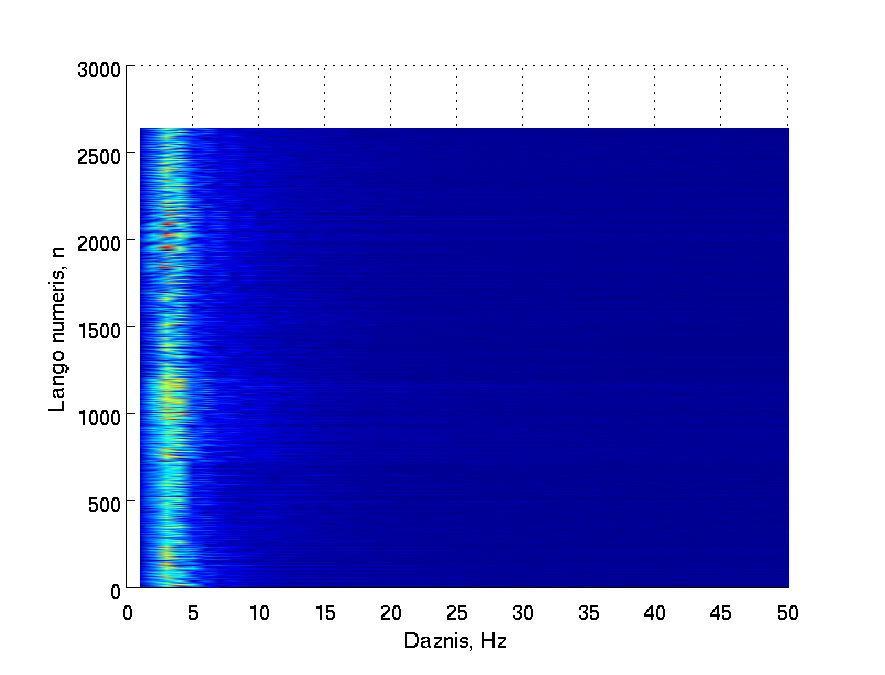
\includegraphics[width=300px]{figures/co_fft.eps}
  \caption{Kontrolinių subjektų kairės kojos žingsnių signalų dažninės komponentės}
  \label{fig:co_fft}
\end{figure}

\begin{figure}[!t]
  \centering
  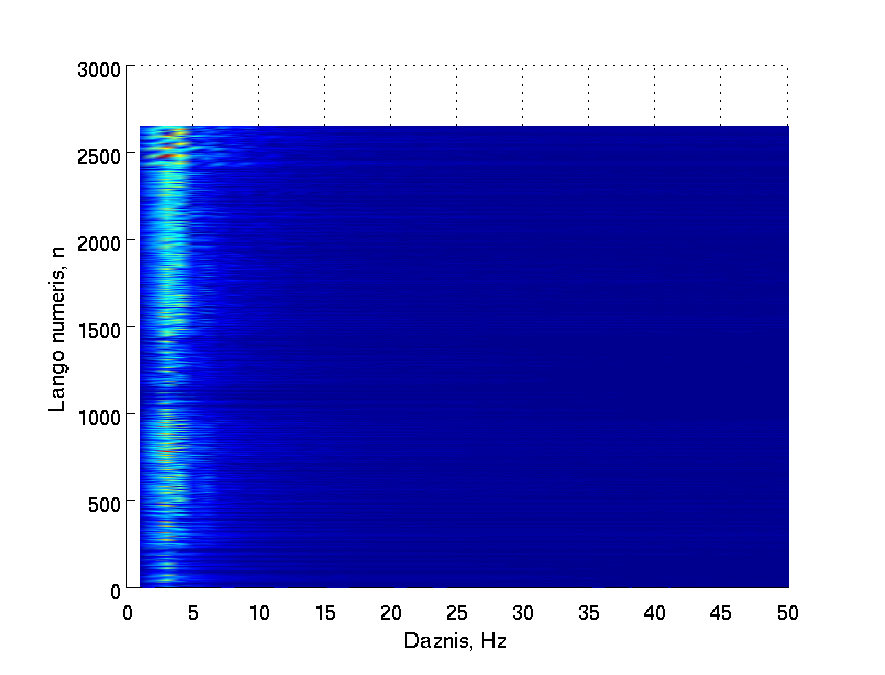
\includegraphics[width=300px]{figures/pt_fft.eps}
  \caption{Parkinsono liga sergančių subjektų kairės kojos žingsnių signalų dažninės komponentės}
  \label{fig:pt_fft}
\end{figure}


Toliau seka išanalizuotos Parkinsono liga sergančių subjektų ir kontrolinių subjektų žingsnių signalų dažninės komponentės. Kontrolinių subjektų kairės kojos žingsnių dažninės komponentės yra pateiktos \ref{fig:co_fft} paveiksle. Parkinsono liga sergančių subjektų kairės kojos žingsnių dažninės komponentės yra pateiktos \ref{fig:pt_fft} paveiksle. Kaip matoma iš duotų komponenčių grafikų -- tiek kontrolinių subjektų, tiek Parkinsono liga sergančių subjektų pagrindinės dažninės komponentės išsidėsto iki $5$ Hz ruože. Ties $0$ Hz dažninių komponenčių nėra, kadangi jos pašalintos filtro pagalba. Už $10$ Hz ribos, komponentės neneša visiškai jokios informacijos. Iš to galima padaryti išvadą, kad tiek Parkinsono liga sergančių subjektų, tiek kontrolinių subjektų eisenos yra visiškai vienodos dažnių srityje ir vien remiantis šita informacija nėra galima nustatyti ar subjektas serga Parkinsono liga ar ne.

Tolimesnė analizė gali būti atlikta, remiantis koreliacijos koeficientais. Analizuojant šiuos požymius, galima remtis tokiu pačiu pirminiu signalo apdorojimo bloku, kaip ir analizuojant dažnines komponentes. Dėl to, kad esama tikrais kairės kojos signalai, galima taikyti tik savi-koreliacijos koeficientus. Narinėjamas požymis parodė gerus klasifikavimo rezultatus ankstesniame tyrime \cite{mano_darbas}, kuriame, remiantis tiesinio pagreičio ir kampinio pagreičio jutiklių parodymais, reikėjo suprojektuoti algoritmą, gebantį atskirti tokias žmogaus veiklas: stovėjimas, ėjimas, ėjimas aukštyn laiptais, ėjimas žemyn laiptais.

\begin{figure}[!t]
  \centering
  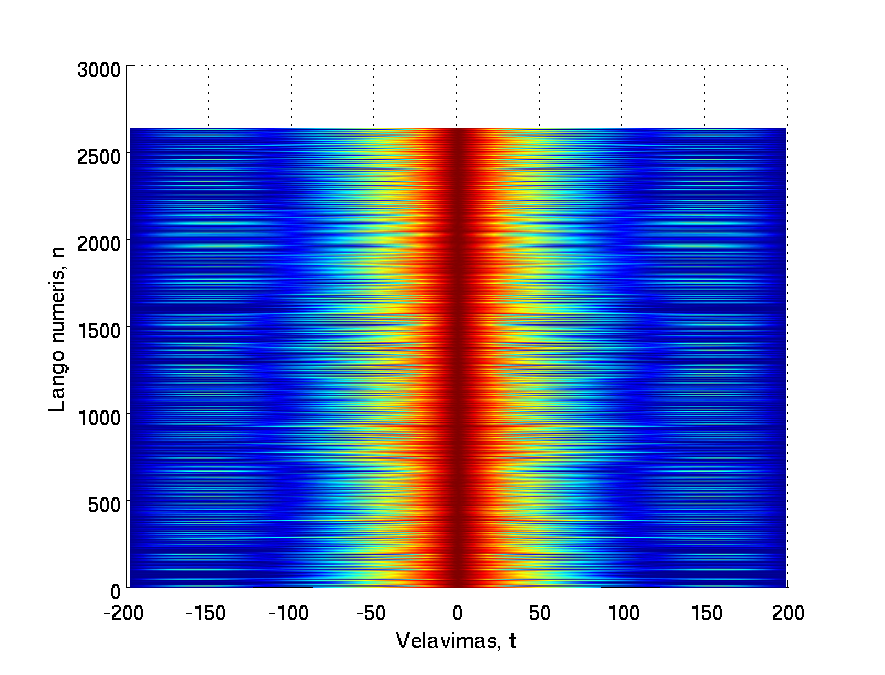
\includegraphics[width=300px]{figures/co_corr.eps}
  \caption{Kontrolinių subjektų kairės kojos žingsnių signalų savi-koreliacijos koeficientai}
  \label{fig:co_corr}
\end{figure}

\begin{figure}[!t]
  \centering
  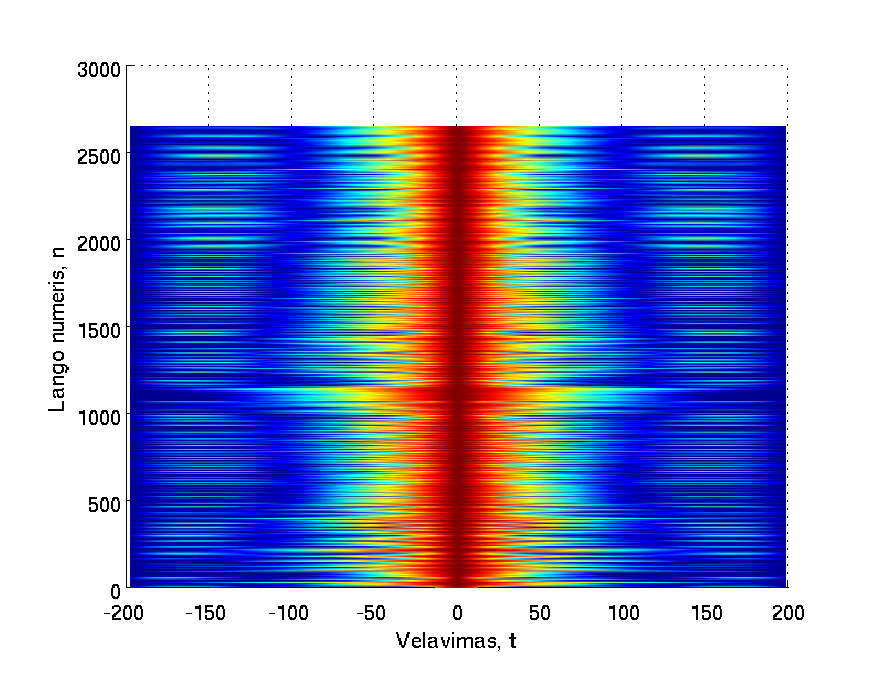
\includegraphics[width=300px]{figures/pt_corr.eps}
  \caption{Parkinsono liga sergančių subjektų kairės kojos žingsnių signalų savi-koreliacijos koeficientai}
  \label{fig:pt_corr}
\end{figure}

Kontrolinių subjektų kairės kojos savi-koreliacijos koeficientai parodyti \ref{fig:co_corr} paveiksle. Parkinsono liga sergančių subjektų kairės kojos savi-koreliacijos koeficientai parodyti \ref{fig:pt_corr} paveiksle. Kaip matyti iš korelogramos, tiek sergantys, tiek kontroliniai subjektai turi panašias, o kai kuriais atvejais ir tokias pačias, koreliacijos reikšmes. Remiantis vien tik turima informacija, nustatyti ar subjektas serga Parkinsono liga ar ne, nėra įmanoma.

\begin{figure}[!t]
  \centering
  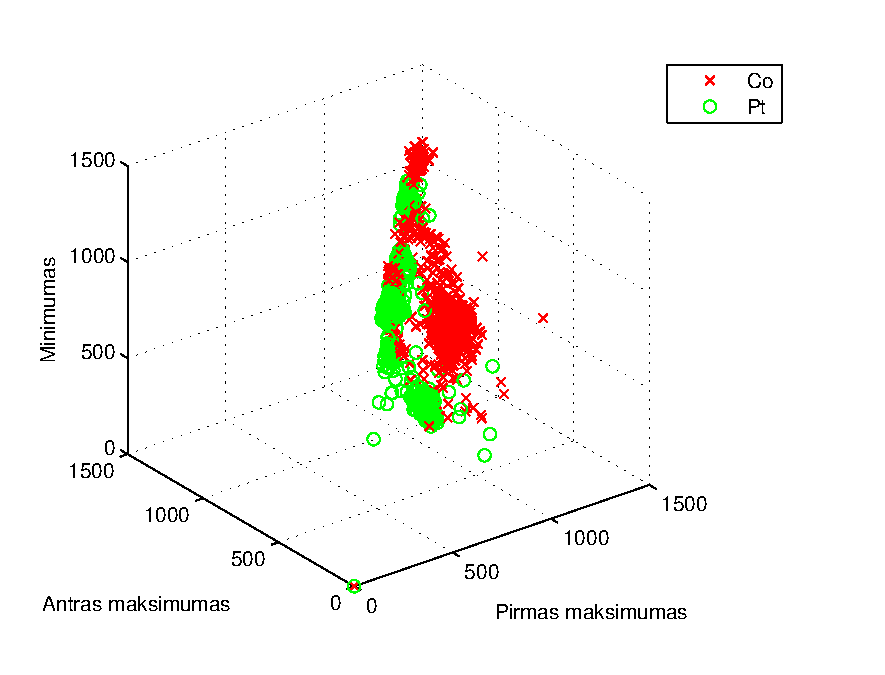
\includegraphics[width=300px]{figures/maximums_minimums.eps}
  \caption{Dviejų globalių maksimumų ir vieno lokalaus minimumo požymių erdvės iliustracija}
  \label{fig:max_min}
\end{figure}

Sudėtingesnė analizė atliekama ieškant sprendimo iš dviejų globalių maksimumų ir vieno lokalaus minimumo požymių erdvės. Šie trys požymiai sudaro trijų matmenų plokštumą, kurią galima lengvai atvaizduoti \ref{fig:max_min} paveiksle. Kaip matyti iš duotos erdvės, duomenys neturi jokio koncentracijos centro. Erdvėje jie pasiskirstę pagal nežinomą dėsnį.

Tokių duomenų pateikti klasifikavimui nėra galima. Grafike ``Co'' taškai, pažymėti kryžiumi, parodo kontrolinį subjektą, ``Pt'' taškai, pažymėti apskritimu, parodo Parkinsono liga sergančius subjektus.

Sekantys požymiai nagrinėjimui yra siūlomos atliktų tyrimų \cite{16053531,KNUTSSON01011972,Delval_Salleron_Bourriez_Bleuse_Moreau_Krystkowiak_Defebvre_Devos_Duhamel_2008}. Nagrinėjamas požymis yra žingsnio fazės laiko variacija. Kojos susilietimo su žeme laiko variacija ir kojos pakilimo nuo žemės laiko variacija.

\begin{figure}[H]
  \centering
%  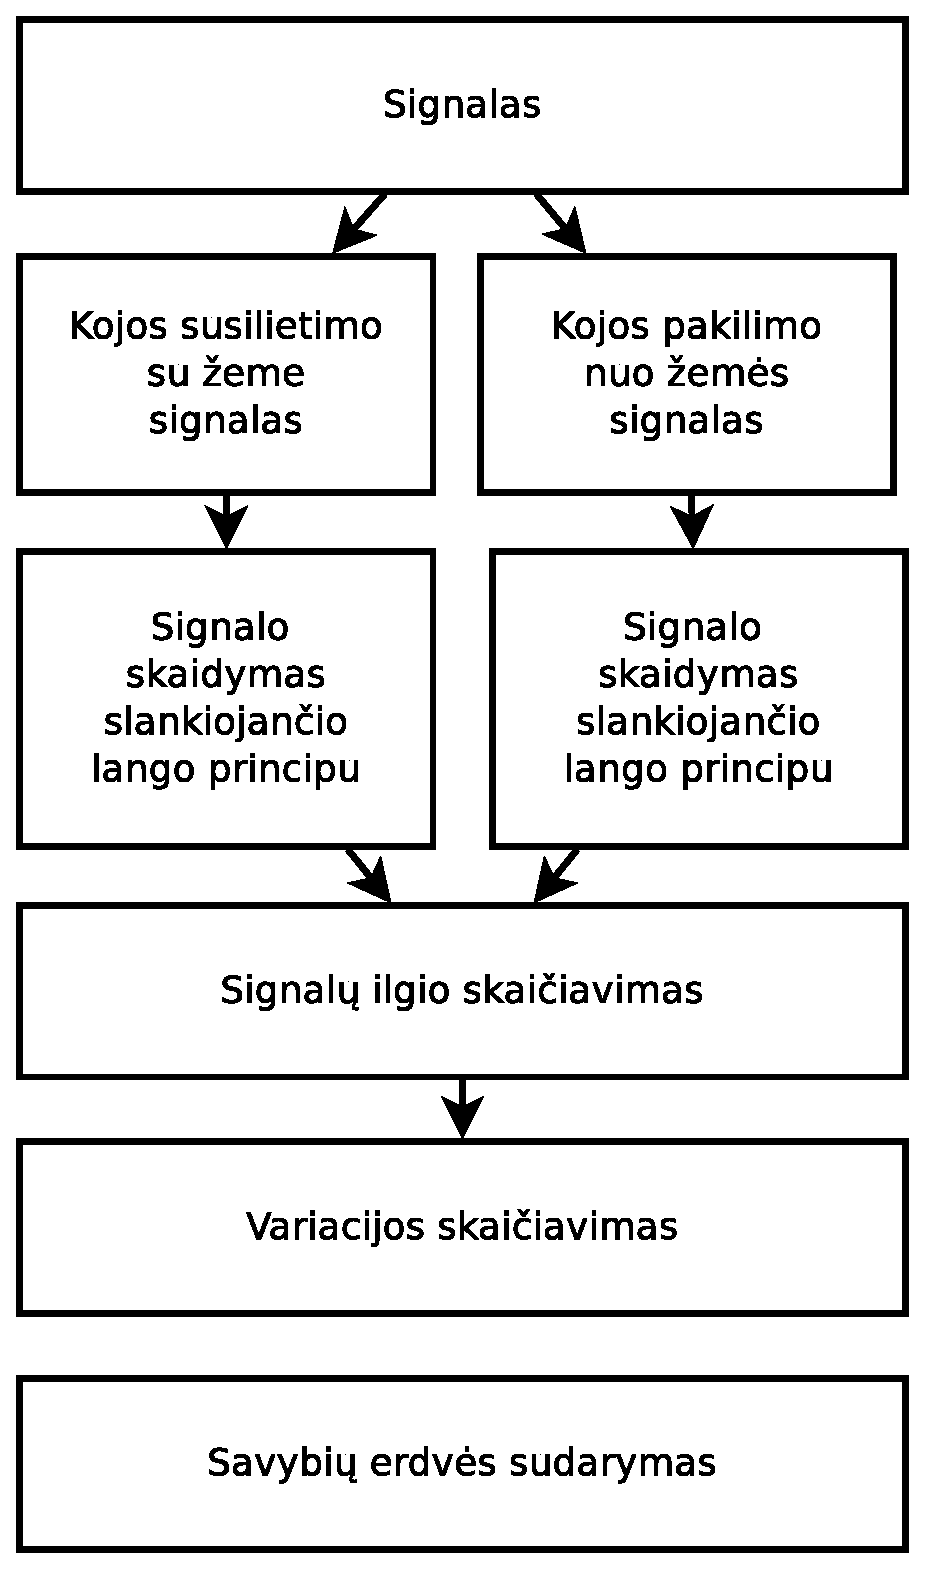
\includegraphics[width=200px]{figures/pirminis_signalo_apdorojimas_skaiciuojant_variacija.eps}
  % Graphic for TeX using PGF
% Title: /home/maksim/Documents/Bbd/3_b/figures/pirminis_signalo_apdorojimas_skaiciuojant_variacija.dia
% Creator: Dia v0.97.2
% CreationDate: Thu May 31 00:41:23 2012
% For: maksim
% \usepackage{tikz}
% The following commands are not supported in PSTricks at present
% We define them conditionally, so when they are implemented,
% this pgf file will use them.
\ifx\du\undefined
  \newlength{\du}
\fi
\setlength{\du}{15\unitlength}
\ttfamily\small
\begin{tikzpicture}
\pgftransformxscale{1.000000}
\pgftransformyscale{-1.000000}
\definecolor{dialinecolor}{rgb}{0.000000, 0.000000, 0.000000}
\pgfsetstrokecolor{dialinecolor}
\definecolor{dialinecolor}{rgb}{1.000000, 1.000000, 1.000000}
\pgfsetfillcolor{dialinecolor}
\definecolor{dialinecolor}{rgb}{1.000000, 1.000000, 1.000000}
\pgfsetfillcolor{dialinecolor}
\fill (10.000000\du,5.000000\du)--(10.000000\du,7.900000\du)--(25.000000\du,7.900000\du)--(25.000000\du,5.000000\du)--cycle;
\pgfsetlinewidth{0.100000\du}
\pgfsetdash{}{0pt}
\pgfsetdash{}{0pt}
\pgfsetmiterjoin
\definecolor{dialinecolor}{rgb}{0.000000, 0.000000, 0.000000}
\pgfsetstrokecolor{dialinecolor}
\draw (10.000000\du,5.000000\du)--(10.000000\du,7.900000\du)--(25.000000\du,7.900000\du)--(25.000000\du,5.000000\du)--cycle;
% setfont left to latex
\definecolor{dialinecolor}{rgb}{0.000000, 0.000000, 0.000000}
\pgfsetstrokecolor{dialinecolor}
\node at (17.500000\du,6.645000\du){Signalas};
\definecolor{dialinecolor}{rgb}{1.000000, 1.000000, 1.000000}
\pgfsetfillcolor{dialinecolor}
\fill (10.000000\du,9.000000\du)--(10.000000\du,13.000000\du)--(17.000000\du,13.000000\du)--(17.000000\du,9.000000\du)--cycle;
\pgfsetlinewidth{0.100000\du}
\pgfsetdash{}{0pt}
\pgfsetdash{}{0pt}
\pgfsetmiterjoin
\definecolor{dialinecolor}{rgb}{0.000000, 0.000000, 0.000000}
\pgfsetstrokecolor{dialinecolor}
\draw (10.000000\du,9.000000\du)--(10.000000\du,13.000000\du)--(17.000000\du,13.000000\du)--(17.000000\du,9.000000\du)--cycle;
% setfont left to latex
\definecolor{dialinecolor}{rgb}{0.000000, 0.000000, 0.000000}
\pgfsetstrokecolor{dialinecolor}
\node at (13.500000\du,10.395000\du){Kojos susilietimo};
% setfont left to latex
\definecolor{dialinecolor}{rgb}{0.000000, 0.000000, 0.000000}
\pgfsetstrokecolor{dialinecolor}
\node at (13.500000\du,11.195000\du){su žeme};
% setfont left to latex
\definecolor{dialinecolor}{rgb}{0.000000, 0.000000, 0.000000}
\pgfsetstrokecolor{dialinecolor}
\node at (13.500000\du,11.995000\du){signalas};
\definecolor{dialinecolor}{rgb}{1.000000, 1.000000, 1.000000}
\pgfsetfillcolor{dialinecolor}
\fill (17.800000\du,9.000000\du)--(17.800000\du,13.000000\du)--(24.800000\du,13.000000\du)--(24.800000\du,9.000000\du)--cycle;
\pgfsetlinewidth{0.100000\du}
\pgfsetdash{}{0pt}
\pgfsetdash{}{0pt}
\pgfsetmiterjoin
\definecolor{dialinecolor}{rgb}{0.000000, 0.000000, 0.000000}
\pgfsetstrokecolor{dialinecolor}
\draw (17.800000\du,9.000000\du)--(17.800000\du,13.000000\du)--(24.800000\du,13.000000\du)--(24.800000\du,9.000000\du)--cycle;
% setfont left to latex
\definecolor{dialinecolor}{rgb}{0.000000, 0.000000, 0.000000}
\pgfsetstrokecolor{dialinecolor}
\node at (21.300000\du,10.395000\du){Kojos pakilimo};
% setfont left to latex
\definecolor{dialinecolor}{rgb}{0.000000, 0.000000, 0.000000}
\pgfsetstrokecolor{dialinecolor}
\node at (21.300000\du,11.195000\du){nuo žemės};
% setfont left to latex
\definecolor{dialinecolor}{rgb}{0.000000, 0.000000, 0.000000}
\pgfsetstrokecolor{dialinecolor}
\node at (21.300000\du,11.995000\du){signalas};
\definecolor{dialinecolor}{rgb}{1.000000, 1.000000, 1.000000}
\pgfsetfillcolor{dialinecolor}
\fill (10.000000\du,14.000000\du)--(10.000000\du,19.000000\du)--(17.000000\du,19.000000\du)--(17.000000\du,14.000000\du)--cycle;
\pgfsetlinewidth{0.100000\du}
\pgfsetdash{}{0pt}
\pgfsetdash{}{0pt}
\pgfsetmiterjoin
\definecolor{dialinecolor}{rgb}{0.000000, 0.000000, 0.000000}
\pgfsetstrokecolor{dialinecolor}
\draw (10.000000\du,14.000000\du)--(10.000000\du,19.000000\du)--(17.000000\du,19.000000\du)--(17.000000\du,14.000000\du)--cycle;
% setfont left to latex
\definecolor{dialinecolor}{rgb}{0.000000, 0.000000, 0.000000}
\pgfsetstrokecolor{dialinecolor}
\node at (13.500000\du,15.495000\du){Signalo };
% setfont left to latex
\definecolor{dialinecolor}{rgb}{0.000000, 0.000000, 0.000000}
\pgfsetstrokecolor{dialinecolor}
\node at (13.500000\du,16.295000\du){skaidymas};
% setfont left to latex
\definecolor{dialinecolor}{rgb}{0.000000, 0.000000, 0.000000}
\pgfsetstrokecolor{dialinecolor}
\node at (13.500000\du,17.095000\du){slankiojančio};
% setfont left to latex
\definecolor{dialinecolor}{rgb}{0.000000, 0.000000, 0.000000}
\pgfsetstrokecolor{dialinecolor}
\node at (13.500000\du,17.895000\du){lango principu};
\definecolor{dialinecolor}{rgb}{1.000000, 1.000000, 1.000000}
\pgfsetfillcolor{dialinecolor}
\fill (18.000000\du,14.000000\du)--(18.000000\du,19.000000\du)--(25.000000\du,19.000000\du)--(25.000000\du,14.000000\du)--cycle;
\pgfsetlinewidth{0.100000\du}
\pgfsetdash{}{0pt}
\pgfsetdash{}{0pt}
\pgfsetmiterjoin
\definecolor{dialinecolor}{rgb}{0.000000, 0.000000, 0.000000}
\pgfsetstrokecolor{dialinecolor}
\draw (18.000000\du,14.000000\du)--(18.000000\du,19.000000\du)--(25.000000\du,19.000000\du)--(25.000000\du,14.000000\du)--cycle;
% setfont left to latex
\definecolor{dialinecolor}{rgb}{0.000000, 0.000000, 0.000000}
\pgfsetstrokecolor{dialinecolor}
\node at (21.500000\du,15.495000\du){Signalo };
% setfont left to latex
\definecolor{dialinecolor}{rgb}{0.000000, 0.000000, 0.000000}
\pgfsetstrokecolor{dialinecolor}
\node at (21.500000\du,16.295000\du){skaidymas};
% setfont left to latex
\definecolor{dialinecolor}{rgb}{0.000000, 0.000000, 0.000000}
\pgfsetstrokecolor{dialinecolor}
\node at (21.500000\du,17.095000\du){slankiojančio};
% setfont left to latex
\definecolor{dialinecolor}{rgb}{0.000000, 0.000000, 0.000000}
\pgfsetstrokecolor{dialinecolor}
\node at (21.500000\du,17.895000\du){lango principu};
\definecolor{dialinecolor}{rgb}{1.000000, 1.000000, 1.000000}
\pgfsetfillcolor{dialinecolor}
\fill (10.000000\du,20.000000\du)--(10.000000\du,22.900000\du)--(25.000000\du,22.900000\du)--(25.000000\du,20.000000\du)--cycle;
\pgfsetlinewidth{0.100000\du}
\pgfsetdash{}{0pt}
\pgfsetdash{}{0pt}
\pgfsetmiterjoin
\definecolor{dialinecolor}{rgb}{0.000000, 0.000000, 0.000000}
\pgfsetstrokecolor{dialinecolor}
\draw (10.000000\du,20.000000\du)--(10.000000\du,22.900000\du)--(25.000000\du,22.900000\du)--(25.000000\du,20.000000\du)--cycle;
% setfont left to latex
\definecolor{dialinecolor}{rgb}{0.000000, 0.000000, 0.000000}
\pgfsetstrokecolor{dialinecolor}
\node at (17.500000\du,21.645000\du){Signalų ilgio skaičiavimas};
\pgfsetlinewidth{0.100000\du}
\pgfsetdash{}{0pt}
\pgfsetdash{}{0pt}
\pgfsetbuttcap
{
\definecolor{dialinecolor}{rgb}{0.000000, 0.000000, 0.000000}
\pgfsetfillcolor{dialinecolor}
% was here!!!
\pgfsetarrowsend{stealth}
\definecolor{dialinecolor}{rgb}{0.000000, 0.000000, 0.000000}
\pgfsetstrokecolor{dialinecolor}
\draw (18.752905\du,7.950189\du)--(19.588330\du,8.950500\du);
}
\pgfsetlinewidth{0.100000\du}
\pgfsetdash{}{0pt}
\pgfsetdash{}{0pt}
\pgfsetbuttcap
{
\definecolor{dialinecolor}{rgb}{0.000000, 0.000000, 0.000000}
\pgfsetfillcolor{dialinecolor}
% was here!!!
\pgfsetarrowsend{stealth}
\definecolor{dialinecolor}{rgb}{0.000000, 0.000000, 0.000000}
\pgfsetstrokecolor{dialinecolor}
\draw (16.181152\du,7.950189\du)--(15.301758\du,8.950500\du);
}
\pgfsetlinewidth{0.100000\du}
\pgfsetdash{}{0pt}
\pgfsetdash{}{0pt}
\pgfsetbuttcap
{
\definecolor{dialinecolor}{rgb}{0.000000, 0.000000, 0.000000}
\pgfsetfillcolor{dialinecolor}
% was here!!!
\pgfsetarrowsend{stealth}
\definecolor{dialinecolor}{rgb}{0.000000, 0.000000, 0.000000}
\pgfsetstrokecolor{dialinecolor}
\draw (21.374536\du,13.049744\du)--(21.407263\du,13.949738\du);
}
\pgfsetlinewidth{0.100000\du}
\pgfsetdash{}{0pt}
\pgfsetdash{}{0pt}
\pgfsetbuttcap
{
\definecolor{dialinecolor}{rgb}{0.000000, 0.000000, 0.000000}
\pgfsetfillcolor{dialinecolor}
% was here!!!
\pgfsetarrowsend{stealth}
\definecolor{dialinecolor}{rgb}{0.000000, 0.000000, 0.000000}
\pgfsetstrokecolor{dialinecolor}
\draw (13.500000\du,13.049744\du)--(13.500000\du,13.949738\du);
}
\pgfsetlinewidth{0.100000\du}
\pgfsetdash{}{0pt}
\pgfsetdash{}{0pt}
\pgfsetbuttcap
{
\definecolor{dialinecolor}{rgb}{0.000000, 0.000000, 0.000000}
\pgfsetfillcolor{dialinecolor}
% was here!!!
\pgfsetarrowsend{stealth}
\definecolor{dialinecolor}{rgb}{0.000000, 0.000000, 0.000000}
\pgfsetstrokecolor{dialinecolor}
\draw (19.439209\du,19.050229\du)--(18.711914\du,19.950256\du);
}
\pgfsetlinewidth{0.100000\du}
\pgfsetdash{}{0pt}
\pgfsetdash{}{0pt}
\pgfsetbuttcap
{
\definecolor{dialinecolor}{rgb}{0.000000, 0.000000, 0.000000}
\pgfsetfillcolor{dialinecolor}
% was here!!!
\pgfsetarrowsend{stealth}
\definecolor{dialinecolor}{rgb}{0.000000, 0.000000, 0.000000}
\pgfsetstrokecolor{dialinecolor}
\draw (15.560791\du,19.050229\du)--(16.288086\du,19.950256\du);
}
\definecolor{dialinecolor}{rgb}{1.000000, 1.000000, 1.000000}
\pgfsetfillcolor{dialinecolor}
\fill (10.000000\du,24.000000\du)--(10.000000\du,26.900000\du)--(25.000000\du,26.900000\du)--(25.000000\du,24.000000\du)--cycle;
\pgfsetlinewidth{0.100000\du}
\pgfsetdash{}{0pt}
\pgfsetdash{}{0pt}
\pgfsetmiterjoin
\definecolor{dialinecolor}{rgb}{0.000000, 0.000000, 0.000000}
\pgfsetstrokecolor{dialinecolor}
\draw (10.000000\du,24.000000\du)--(10.000000\du,26.900000\du)--(25.000000\du,26.900000\du)--(25.000000\du,24.000000\du)--cycle;
% setfont left to latex
\definecolor{dialinecolor}{rgb}{0.000000, 0.000000, 0.000000}
\pgfsetstrokecolor{dialinecolor}
\node at (17.500000\du,25.645000\du){Variacijos skaičiavimas};
\pgfsetlinewidth{0.100000\du}
\pgfsetdash{}{0pt}
\pgfsetdash{}{0pt}
\pgfsetbuttcap
{
\definecolor{dialinecolor}{rgb}{0.000000, 0.000000, 0.000000}
\pgfsetfillcolor{dialinecolor}
% was here!!!
\pgfsetarrowsend{stealth}
\definecolor{dialinecolor}{rgb}{0.000000, 0.000000, 0.000000}
\pgfsetstrokecolor{dialinecolor}
\draw (17.500000\du,22.950488\du)--(17.500000\du,23.949512\du);
}
\definecolor{dialinecolor}{rgb}{1.000000, 1.000000, 1.000000}
\pgfsetfillcolor{dialinecolor}
\fill (10.000000\du,28.000000\du)--(10.000000\du,30.900000\du)--(25.000000\du,30.900000\du)--(25.000000\du,28.000000\du)--cycle;
\pgfsetlinewidth{0.100000\du}
\pgfsetdash{}{0pt}
\pgfsetdash{}{0pt}
\pgfsetmiterjoin
\definecolor{dialinecolor}{rgb}{0.000000, 0.000000, 0.000000}
\pgfsetstrokecolor{dialinecolor}
\draw (10.000000\du,28.000000\du)--(10.000000\du,30.900000\du)--(25.000000\du,30.900000\du)--(25.000000\du,28.000000\du)--cycle;
% setfont left to latex
\definecolor{dialinecolor}{rgb}{0.000000, 0.000000, 0.000000}
\pgfsetstrokecolor{dialinecolor}
\node at (17.500000\du,29.645000\du){Savybių erdvės sudarymas};
\pgfsetlinewidth{0.100000\du}
\pgfsetdash{}{0pt}
\pgfsetdash{}{0pt}
\pgfsetbuttcap
{
\definecolor{dialinecolor}{rgb}{0.000000, 0.000000, 0.000000}
\pgfsetfillcolor{dialinecolor}
% was here!!!
\pgfsetarrowsend{stealth}
\definecolor{dialinecolor}{rgb}{0.000000, 0.000000, 0.000000}
\pgfsetstrokecolor{dialinecolor}
\draw (17.500000\du,26.950488\du)--(17.500000\du,27.949512\du);
}
\end{tikzpicture}

  \caption{Pirminis signalo apdorojimas, išskiriant kojos susilietimo su žeme laiko ir kojos pakilimo nuo žemės laiko variacijos požymiai}
  \label{fig:stance_swing_extract}
\end{figure}

Išskiriant variacijos požymį iš signalo, reikalinga pakeisti pirminio signalo apdorojimo algoritmą. Kadangi kojos pakilimas nuo žemės ir kojos susilietimas su žeme gali būti vienas nuo kito nepriklausomi (subjektas sustojo ir stovi dviem kojomis ant žemės arba subjektas stovi tik ant kairės kojos), pirminis signalo apdorojimas turi būti atliekamas lygiagrečiai, t.y. tuo pat metu išskiriamas tiek kojos pakilimo nuo žemės signalas, tiek ir kojos susilietimas su žeme signalas. Tokios sistemos struktūrinis grafikas yra parodytas \ref{fig:stance_swing_extract} paveiksle. Kitas žingsnis yra signalo išskaidymas slankiojančio lango principu. Abiejų signalų slankiojančio lango ilgis parinktas $4$ verčių ilgio, su $2$ verčių perdanga. Kuomet tiek kojos susilietimo su žeme, tiek kojos pakilimo nuo žemės keturi signalai patenkina keliamus reikalavimus -- iš jų yra apskaičiuojami signalų ilgiai. Vėliau, abiejų etapų signalams yra paskaičiuojama jų variacija ir sudaroma požymių erdvė. Toliau nagrinėjamos abiejų signalų variacijos vieno matmens plokštumoje.

\begin{figure}[!t]
  \centering
  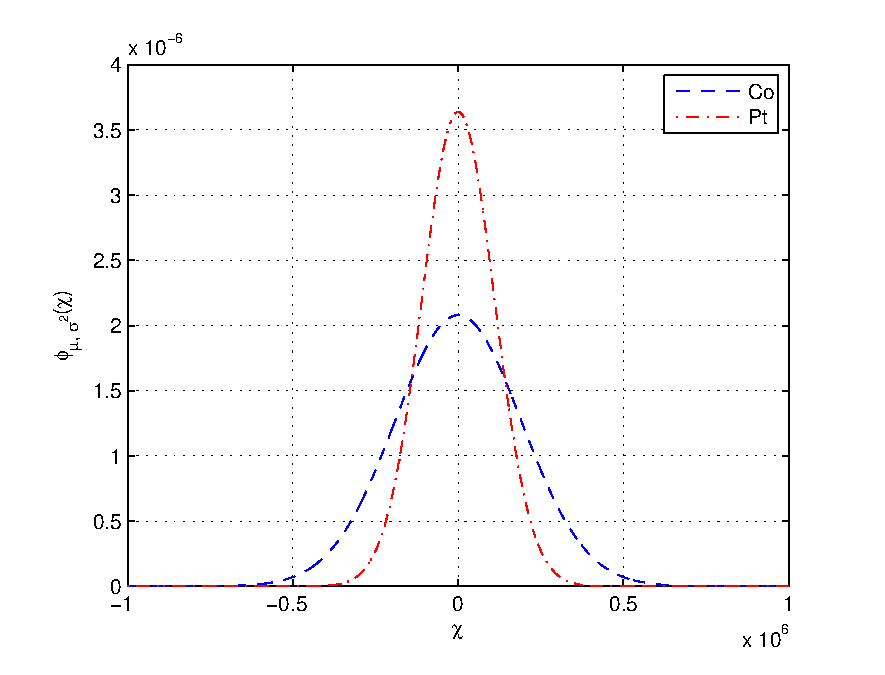
\includegraphics[width=250px]{figures/stance_phase.eps}
  \caption{Kojos prisilietimo prie žemės laiko variacija}
  \label{fig:stance_var}
\end{figure}

Abiejų signalų variacijų pasiskirstymai yra parodyti \ref{fig:stance_var} ir \ref{fig:swing_var} paveiksluose. Abu pasiskirstymai turi vieną trūkumą -- jų vidurkiai sutampa, tačiau gera žinia yra tai, kad jų variacijos skirtingos. Norint išspręsti iškilusią problemą, reikia taikyti matmenų praskyrimo metodus. Darbo metu išbandyti tokie matmenų praskyrimo metodai:

\begin{itemize}
\item PCA;
\item LDA;
\item Kernel PCA (su daugianariu, Gauso branduoliais);
\item Kernel LDA (su daugianariu, Gauso branduoliais);
\end{itemize}

\begin{figure}[!t]
  \centering
  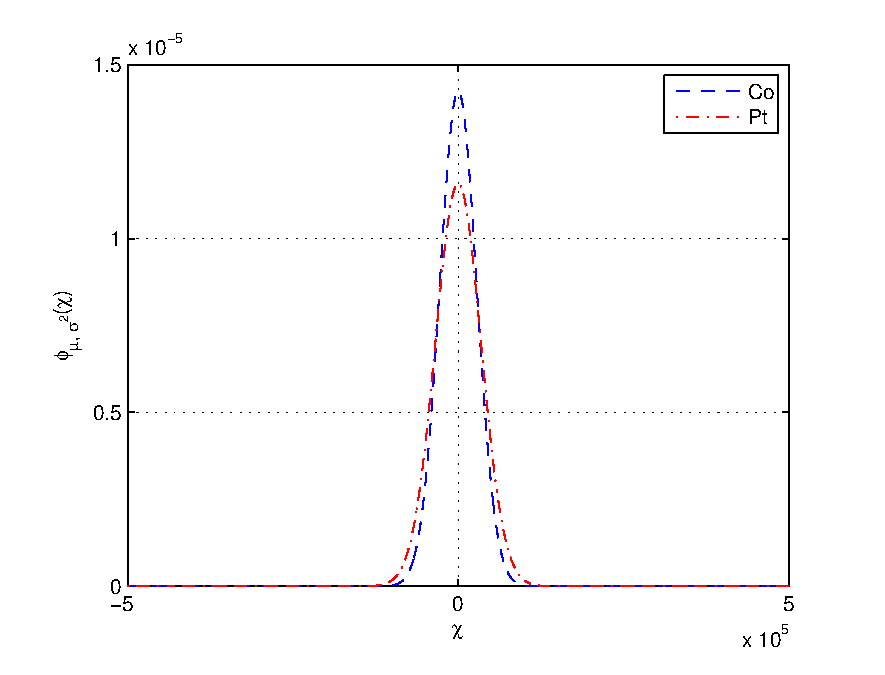
\includegraphics[width=250px]{figures/swing_phase.eps}
  \caption{Kojos pakilimo nuo žemės laiko variacija}
  \label{fig:swing_var}
\end{figure}

\begin{figure}[!t]
  \centering
  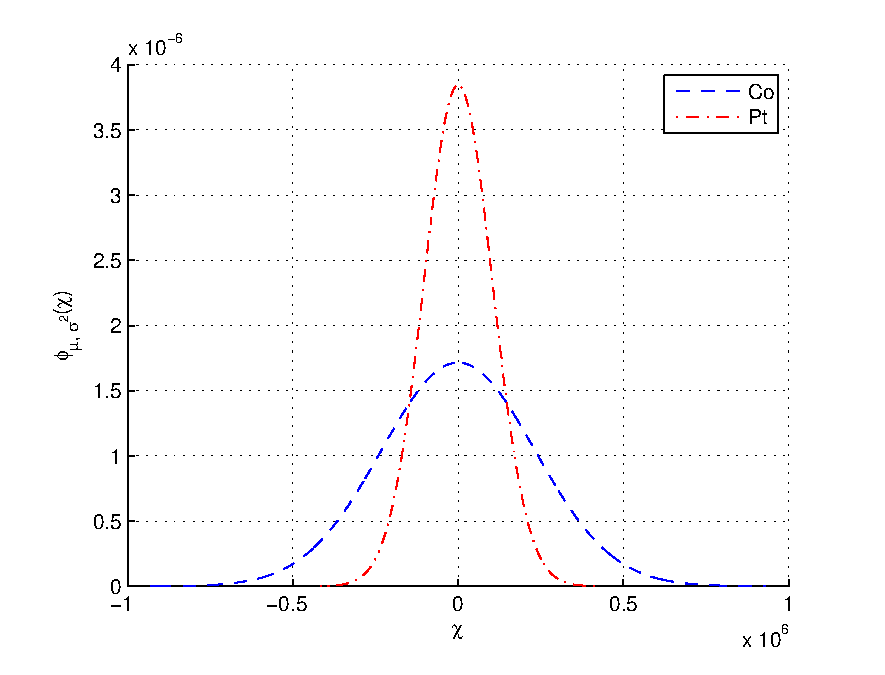
\includegraphics[width=250px]{figures/st_sw_linear_kpca.eps}
  \caption{Kojos prisilietimo prie žemės ir pakilimo nuo žemės laiko variacijos pasiskirstymas po PCA transformacijos}
  \label{fig:linear_pca}
\end{figure}

Vienmatė tiesinė PCA transformacija atvaizduota \ref{fig:linear_pca} paveiksle. Vizualiai įvertinus gaunamą grafiką -- vidurkis nepasikeitė, tačiau pakito variacija. Vidurkio pokyčio nėra pastebima, todėl teikti duomenis klasifikavimui nėra prasmės, kadangi to pačio vidurkio duomenis atskirti nėra įmanoma.

\begin{figure}[!t]
  \centering
  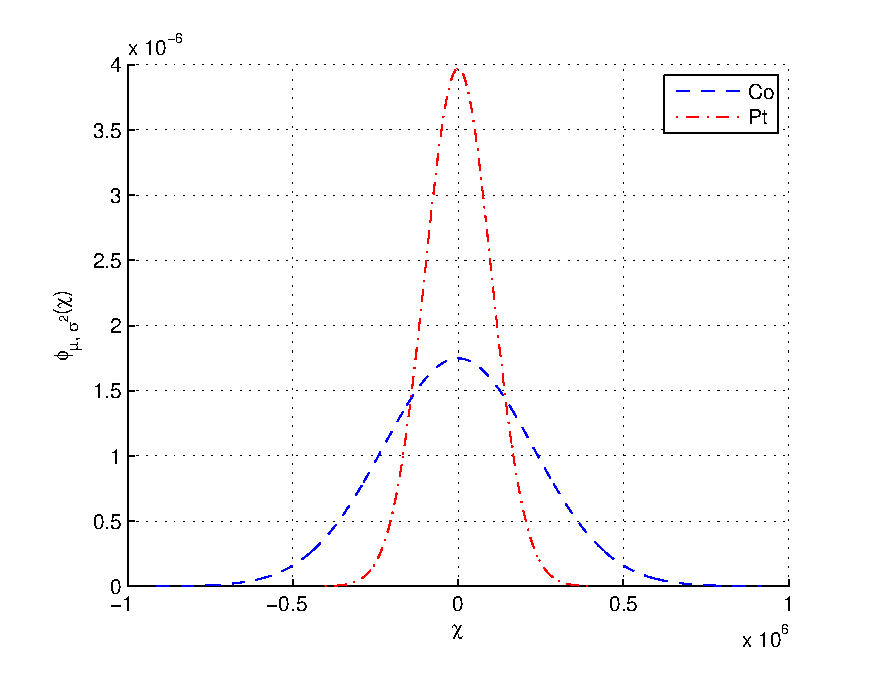
\includegraphics[width=250px]{figures/st_sw_linear_lda.eps}
  \caption{Kojos prisilietimo prie žemės ir pakilimo nuo žemės laiko variacijos pasiskirstymas po LDA transformacijos}
  \label{fig:linear_lda}
\end{figure}

Kitas metodas yra LDA. Transformacijos rezultatas yra pavaizduotas \ref{fig:linear_lda} paveiksle. Vizualiai įvertinus gaunamą grafiką -- tiek po LDA, tiek po PCA duomenų pasiskirstymas nėra gerai atskirtas. Galima daryti hipotezę, kad tiesinis duomenų atskyrimas šiuo atveju naudoti nėra tinkamas. Reikia papildyti transformacijas naudojant daugianarį arba Gauso branduolį.

\begin{figure}[!t]
  \centering
  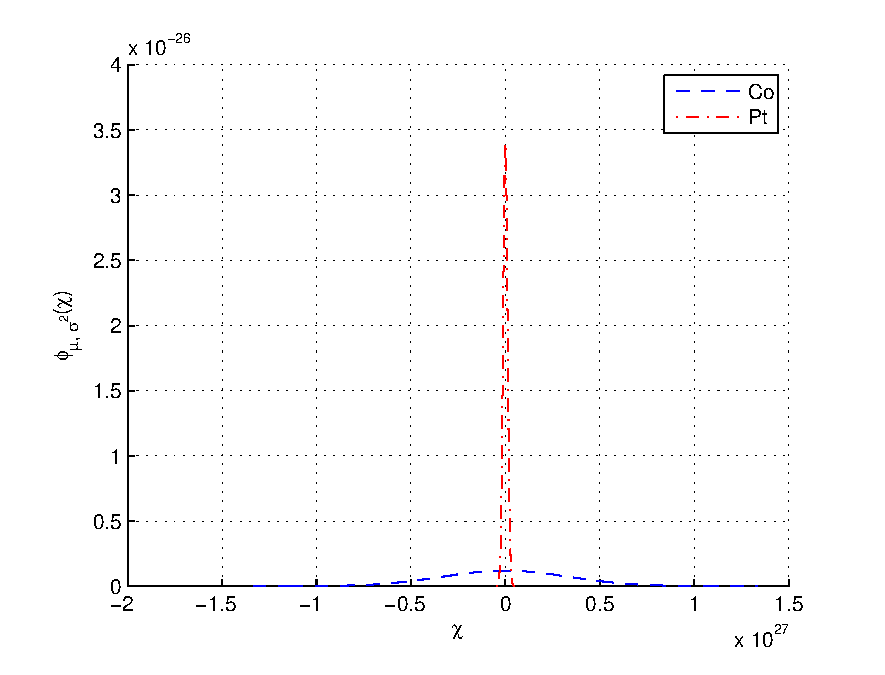
\includegraphics[width=250px]{figures/st_sw_poly_kpca.eps}
  \caption{Kojos prisilietimo prie žemės ir pakilimo nuo žemės laiko variacijos pasiskirstymas po PCA transformacijos, naudojant daugianarį branduolį}
  \label{fig:poly_pca}
\end{figure}

\begin{figure}[!t]
  \centering
  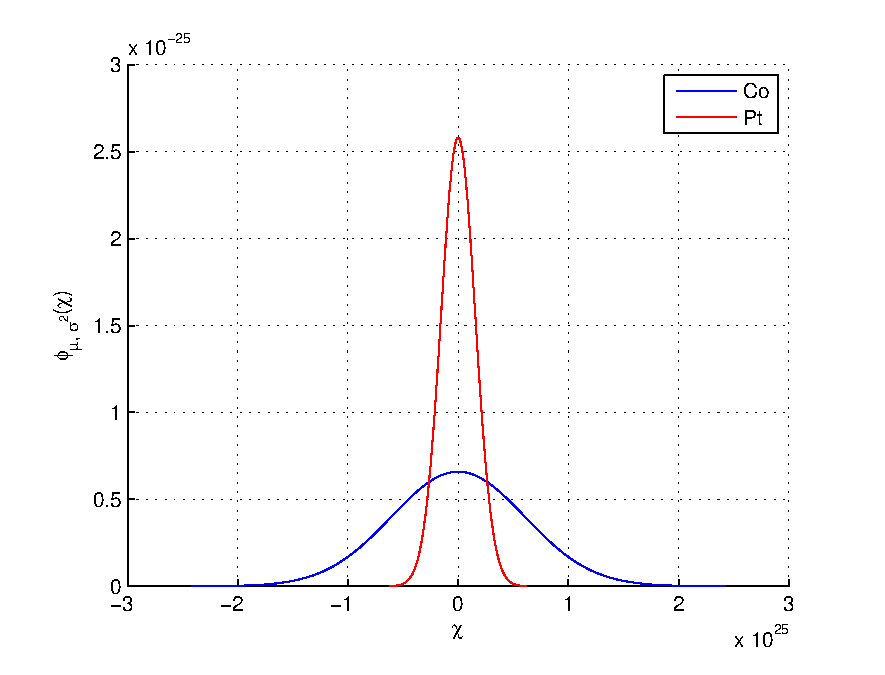
\includegraphics[width=250px]{figures/st_sw_poly_gda.eps}
  \caption{Kojos prisilietimo prie žemės ir pakilimo nuo žemės laiko variacijos pasiskirstymas po LDA transformacijos, naudojant daugianarį branduolį}
  \label{fig:poly_lda}
\end{figure}

Branduolio metodas pritaikytas PCA transformacijai yra atvaizduotas \ref{fig:poly_pca} ir \ref{fig:gauss_pca} paveiksluose. Branduolio metodas pritaikytas LDA transformacijai yra atvaizduotas \ref{fig:poly_lda} ir \ref{fig:gauss_pca} paveiksluose. Daugianaris branduolys abiems atvejais panaudotas su 4 branduolio argumentu.

\begin{figure}[!t]
  \centering
  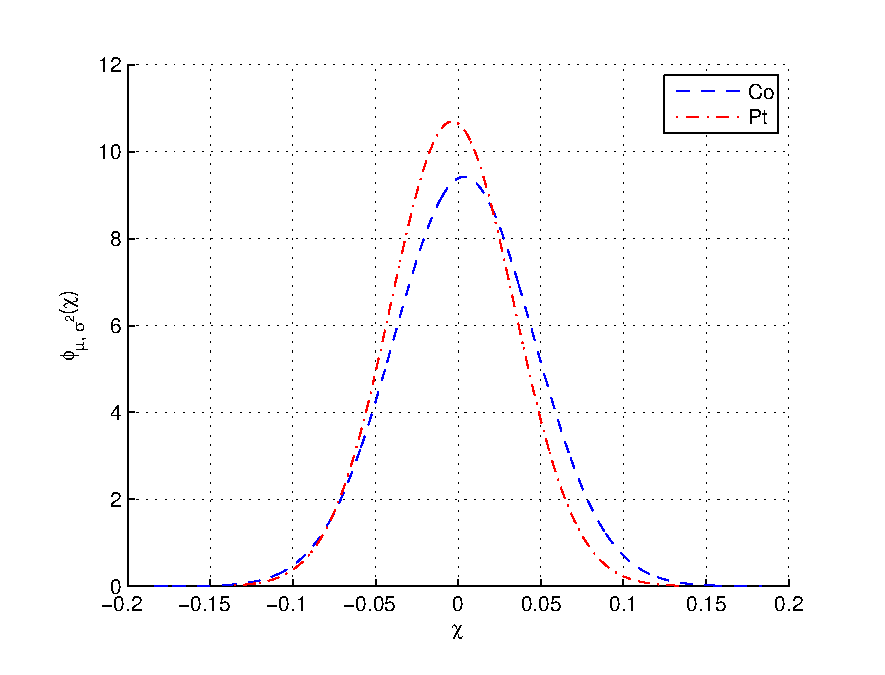
\includegraphics[width=250px]{figures/st_sw_gauss_kpca.eps}
  \caption{Kojos prisilietimo prie žemės ir pakilimo nuo žemės laiko variacijos pasiskirstymas po PCA transformacijos, naudojant Gauso branduolį}
  \label{fig:gauss_pca}
\end{figure}

\begin{figure}[!t]
  \centering
  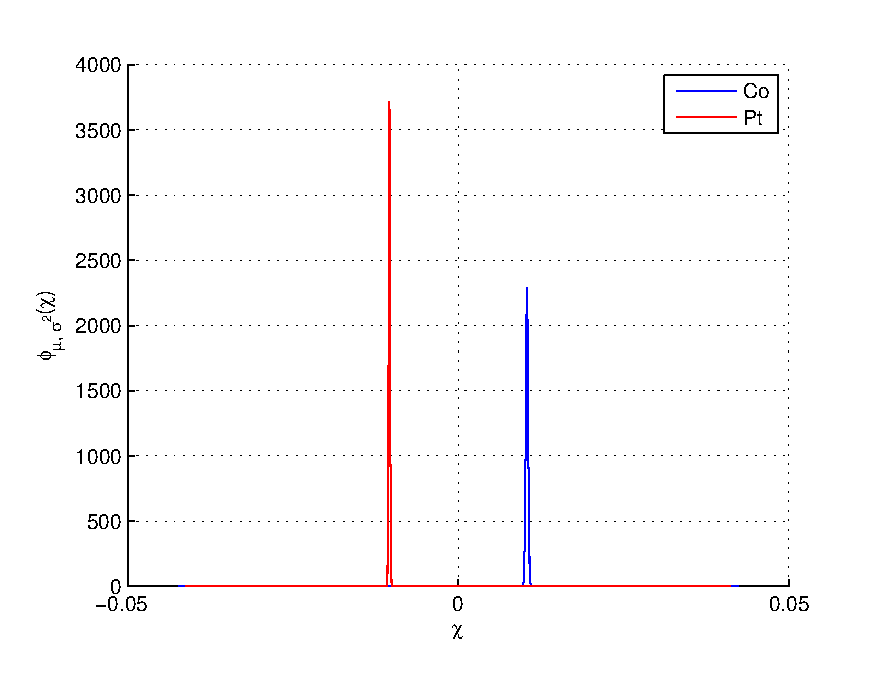
\includegraphics[width=250px]{figures/st_sw_gauss_gda.eps}
  \caption{Kojos prisilietimo prie žemės ir pakilimo nuo žemės laiko variacijos pasiskirstymas po LDA transformacijos, naudojant Gauso branduolį}
  \label{fig:gauss_lda}
\end{figure}

Vizualiai įvertinus gaunamą grafiką, panaudojus daugianarį branduolį, tiek PCA (\ref{fig:poly_pca} paveikslas), tiek LDA (\ref{fig:poly_lda} paveikslas) atveju -- vidurkis iš savo vietos nepajudėjo. Abi transformacijos pakeitė variaciją. Norimas tikslas nėra pasiektas, todėl toks branduolys nėra tinkamas. Panaudojus Gauso branduolį rezultatas pagerėja LDA transformacijos atveju (\ref{fig:gauss_lda} paveikslas), PCA su tokiu branduoliu (\ref{fig:gauss_pca} paveikslas) duomenis tik dar labiau suvienodina.

Remiantis pateikta analize galima teigti, kad geriausiai duomenis požymių erdvėje atskiria LDA su Gauso branduoliu. Tolimesniame darbe duomenis į klasifikatorių pateikiami po tokio tipo transformacijos.

\subsection{Požymių klasifikavimo programos kūrimas}

Šiame skyriuje išnagrinėti ir pritaikyti populiariausi šiuo metu naudojami klasifikatorių metodai. Tokie klasifikatoriai yra \cite{824819}:

\begin{itemize}
\item Atraminių vektorių mašina (angl. \textit{Support Vector Machine -- SVM});
\item Paslėptas Markovo modelis (angl. \textit{Hidden Markov Model -- HMM});
\item Naivusis Bayes klasifikatorius (angl. \textit{NayveBayes});
\item Tiesioginio sklidimo neuronų tinklas (angl. \textit{Feed-Forward Neural Network -- FFNN}).
\end{itemize}

Labai svarbu yra atskirti duomenis, kuriais klasifikatorius yra apmokamas ir kuriais jis yra testuojamas. Jeigu klasifikatoriaus apmokymo duomenys yra pakankamai apibendrinti, tuomet naujus duomenis klasifikatorius turėtų gerai atpažinti. Pateikiant klasifikatoriaus testavime tokius pačius duomenis, kaip ir apmokyme -- atliekamas tikrinimas ar klasifikatorius teisingai ``suprato'' nagrinėjamus duomenis, tačiau tai neapibrėžia kiek gerai jis apdoros naujus duomenis.

Nurodytų klasifikatorių veikimas vertinamas tikslumu ir klasės atpažinimu. Tikslumas apskaičiuojamas:

\begin{equation}
Tikslumas = \frac{T_P + T_N}{T_P + F_P + T_N + F_N},
\end{equation}
kur $T_P$ -- teisingai identifikuotų klasių skaičius, $T_N$ -- teisingai atmestų klasių skaičius, $F_P$ -- klaidingai identifikuotų klasių skaičius ir $F_N$ -- klaidingai atmestų klasių skaičius.

Atpažinimas apskaičiuojamas:

\begin{equation}
Atpažinimas = \frac{T_P}{T_P + F_P}
\end{equation}

Visos tolesnės klasifikatorių patikros atliekamos remiantis tokia schema: iš turimų duomenų išskirta kojos prisilietimo ir pakilimo nuo žemės laiko ilgio variacijos požymiai. Visi duomenys padalinti į lygias tris dalis: matmenų operacijai atlikti duota $500$ reikšmių, klasifikatoriaus apmokymui tolimesnės eilės $500$ reikšmių, klasifikatoriaus testavimui tolimesnės eilės $500$ reikšmių. Klasifikavimas atliekamas realiu laiku, t.y. klasifikatoriui pateikiami duomenis apie žingsnio stadijos variaciją po transformacijos ir klasifikatorius pateikia savo spėjimą.

Atraminių vektorių mašina \cite{Burges98atutorial} šiuo metu yra populiariausias klasifikatorius nagrinėjant netiesiškai atskiriamus duomenis. Įgyvendinimas Matlab aplinkoje panaudotas iš literatūroje pateikto metodo \cite{website:svm_implementation}. Klasifikatoriaus testavimo metu naudojami tokie parametrai:

\begin{itemize}
\item SVM tipas -- Siquential Minimal Optimization;
\item Branduolio tipas -- tiesinis;
\item Sureguliavimo konstanta -- 2;
\item Branduolio argumentas -- 2.
\end{itemize}

Lentelėje \ref{table:svm_scores} pateikti SVM tikslumo ir atpažinimo duomenys. Kaip matyti, klasifikatorius veikia nepakankamai gerai -- tikslumo koeficientas nėra didesnis negu pusė, abiems atvejams tik $0,489$. Pirmos klasės atpažinimas $0,234$, antros klasės atpažinimas $0,744$, tačiau to nepakanka. Iš padarytos klasifikatoriaus veikimo analizės galima teigti, kad klasifikatorius veikia blogai ir jo naudoti sprendime nėra galima.

\begin{table}[!t]
  \centering
  \renewcommand{\arraystretch}{1.3}
  \caption{Vektoriaus palaikymo mašinos klasifikavimo rezultatas}
  \label{table:svm_scores}
  \begin{tabular}{|c|c|c|} \hline
    & Co & Pt \\ \hline
    Tikslumas & 0,489 & 0,489 \\ \hline
    Atpažinimas & 0,234 & 0,744 \\ \hline
  \end{tabular}
\end{table}

Paslėptas Markovo modelis \cite{18626} yra vienintelis iš šiame darbe nagrinėjamų klasifikatorių, kuris turi laikinę informaciją. Tokia savybė suteikia ``inkaro'' galimybę -- klasifikatorius gali užsilaikyti prie vienos klasės net ir tuomet, kai pagal požymių erdvę turi būti kita duomenų grupė. Tokia klasifikatoriaus savybė pritaikyta ankstesniame darbe, sudarant žmogaus eisenos atpažinimo sprendimą \cite{mano_darbas}. Pasirinktas modelis, susidedantis iš dviejų būsenų -- ``Sveikas'', ``Sergantis''. Būsenos tarpusavyje yra sujungtos (\ref{fig:hmm_model} paveikslas). Perėjimo tikimybės tarp modelio elementų parinktos žymiai mažesnės už tikimybę likti toje pačioje būsenoje. Įgyvendinimas Matlab aplinkoje panaudotas iš \cite{website:hmm_implementation}.

\begin{figure}
	\centering
%	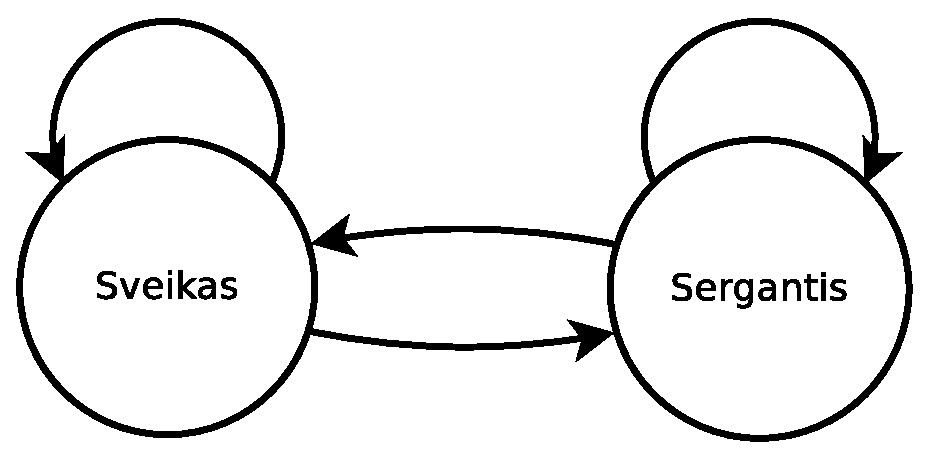
\includegraphics[width=250px]{figures/hmm_modelis}
	% Graphic for TeX using PGF
% Title: /home/maksim/Documents/Bbd/3_b/figures/hmm_modelis.dia
% Creator: Dia v0.97.2
% CreationDate: Thu May 31 00:46:40 2012
% For: maksim
% \usepackage{tikz}
% The following commands are not supported in PSTricks at present
% We define them conditionally, so when they are implemented,
% this pgf file will use them.
\ifx\du\undefined
  \newlength{\du}
\fi
\setlength{\du}{15\unitlength}
\ttfamily\small
\begin{tikzpicture}
\pgftransformxscale{1.000000}
\pgftransformyscale{-1.000000}
\definecolor{dialinecolor}{rgb}{0.000000, 0.000000, 0.000000}
\pgfsetstrokecolor{dialinecolor}
\definecolor{dialinecolor}{rgb}{1.000000, 1.000000, 1.000000}
\pgfsetfillcolor{dialinecolor}
\definecolor{dialinecolor}{rgb}{1.000000, 1.000000, 1.000000}
\pgfsetfillcolor{dialinecolor}
\pgfpathellipse{\pgfpoint{17.500000\du}{12.500000\du}}{\pgfpoint{2.500000\du}{0\du}}{\pgfpoint{0\du}{2.500000\du}}
\pgfusepath{fill}
\pgfsetlinewidth{0.100000\du}
\pgfsetdash{}{0pt}
\pgfsetdash{}{0pt}
\pgfsetmiterjoin
\definecolor{dialinecolor}{rgb}{0.000000, 0.000000, 0.000000}
\pgfsetstrokecolor{dialinecolor}
\pgfpathellipse{\pgfpoint{17.500000\du}{12.500000\du}}{\pgfpoint{2.500000\du}{0\du}}{\pgfpoint{0\du}{2.500000\du}}
\pgfusepath{stroke}
% setfont left to latex
\definecolor{dialinecolor}{rgb}{0.000000, 0.000000, 0.000000}
\pgfsetstrokecolor{dialinecolor}
\node at (17.500000\du,12.695000\du){Sveikas};
\definecolor{dialinecolor}{rgb}{1.000000, 1.000000, 1.000000}
\pgfsetfillcolor{dialinecolor}
\pgfpathellipse{\pgfpoint{27.530842\du}{12.530842\du}}{\pgfpoint{2.530842\du}{0\du}}{\pgfpoint{0\du}{2.530842\du}}
\pgfusepath{fill}
\pgfsetlinewidth{0.100000\du}
\pgfsetdash{}{0pt}
\pgfsetdash{}{0pt}
\pgfsetmiterjoin
\definecolor{dialinecolor}{rgb}{0.000000, 0.000000, 0.000000}
\pgfsetstrokecolor{dialinecolor}
\pgfpathellipse{\pgfpoint{27.530842\du}{12.530842\du}}{\pgfpoint{2.530842\du}{0\du}}{\pgfpoint{0\du}{2.530842\du}}
\pgfusepath{stroke}
% setfont left to latex
\definecolor{dialinecolor}{rgb}{0.000000, 0.000000, 0.000000}
\pgfsetstrokecolor{dialinecolor}
\node at (27.530842\du,12.725842\du){Sergantis};
\pgfsetlinewidth{0.100000\du}
\pgfsetdash{}{0pt}
\pgfsetdash{}{0pt}
\pgfsetbuttcap
{
\definecolor{dialinecolor}{rgb}{0.000000, 0.000000, 0.000000}
\pgfsetfillcolor{dialinecolor}
% was here!!!
\pgfsetarrowsend{stealth}
\definecolor{dialinecolor}{rgb}{0.000000, 0.000000, 0.000000}
\pgfsetstrokecolor{dialinecolor}
\pgfpathmoveto{\pgfpoint{19.935988\du}{13.251029\du}}
\pgfpatharc{102}{79}{13.077237\du and 13.077237\du}
\pgfusepath{stroke}
}
\pgfsetlinewidth{0.100000\du}
\pgfsetdash{}{0pt}
\pgfsetdash{}{0pt}
\pgfsetbuttcap
{
\definecolor{dialinecolor}{rgb}{0.000000, 0.000000, 0.000000}
\pgfsetfillcolor{dialinecolor}
% was here!!!
\pgfsetarrowsend{stealth}
\definecolor{dialinecolor}{rgb}{0.000000, 0.000000, 0.000000}
\pgfsetstrokecolor{dialinecolor}
\pgfpathmoveto{\pgfpoint{25.063657\du}{11.773448\du}}
\pgfpatharc{282}{259}{13.077237\du and 13.077237\du}
\pgfusepath{stroke}
}
\pgfsetlinewidth{0.100000\du}
\pgfsetdash{}{0pt}
\pgfsetdash{}{0pt}
\pgfsetbuttcap
{
\definecolor{dialinecolor}{rgb}{0.000000, 0.000000, 0.000000}
\pgfsetfillcolor{dialinecolor}
% was here!!!
\pgfsetarrowsend{stealth}
\definecolor{dialinecolor}{rgb}{0.000000, 0.000000, 0.000000}
\pgfsetstrokecolor{dialinecolor}
\pgfpathmoveto{\pgfpoint{19.267722\du}{10.732374\du}}
\pgfpatharc{25}{-204}{1.938014\du and 1.938014\du}
\pgfusepath{stroke}
}
\pgfsetlinewidth{0.100000\du}
\pgfsetdash{}{0pt}
\pgfsetdash{}{0pt}
\pgfsetbuttcap
{
\definecolor{dialinecolor}{rgb}{0.000000, 0.000000, 0.000000}
\pgfsetfillcolor{dialinecolor}
% was here!!!
\pgfsetarrowsend{stealth}
\definecolor{dialinecolor}{rgb}{0.000000, 0.000000, 0.000000}
\pgfsetstrokecolor{dialinecolor}
\pgfpathmoveto{\pgfpoint{29.320323\du}{10.741476\du}}
\pgfpatharc{24}{-203}{1.954759\du and 1.954759\du}
\pgfusepath{stroke}
}
\end{tikzpicture}

	\caption{Ergodinis paslėptas Markovo modelis}
	\label{fig:hmm_model}
\end{figure}

Lentelėje \ref{table:hmm_scores} pateikti tikslumo ir taikumo duomenys. Kaip matyti iš tikslumo rezultato -- klasifikatorius teisingai priskiria atsakymą tik pusei duomenų. Iš to galime teigti, kad klasifikatorius yra labai blogai apmokytas ir visiškai nesugeba apibendrinti turimų duomenų. Klasifikatorius visus pateikiamus testavimo duomenis priskiria vienai klasei.

\begin{table}
  \centering
  \renewcommand{\arraystretch}{1.3}
  \caption{Paslėpto Markovo modelio klasifikavimo rezultatas}
  \label{table:hmm_scores}
  \begin{tabular}{|c|c|c|} \hline
    & Co & Pt \\ \hline
    Tikslumas & 0,500 & 0,500 \\ \hline
    Atpažinimas & 0,000 & 1,000 \\ \hline
  \end{tabular}
\end{table}

Naivus Bayes \cite{R22230} yra vienas iš pirmųjų statistinių metodų grindžiamų klasifikavimo mechanizmas. Jis veikia labai paprastai -- ieškoma tiesinės funkcijos, kuri geriausiai atskiria nagrinėjamus duomenis ir vieni žymenis priskiriami, jeigu duomenys yra vienoje linijos pusėje, atvirkšti žymenis priskiriami, jeigu duomenys yra kitoje linijos pusėje. 

Lentelėje \ref{table:nb_scores} pateikti tikslumo ir atpažinimo duomenys. Tikslumo koeficientas viršija pusę, $0,508$, tačiau tai yra mažai. Atpažinimo koeficientas pirmuoju atveju yra neblogas, $0,764$, tačiau antruoju atveju koeficientas yra visiškai nepatenkinamas, viso $0,252$. Iš turimų rezultatų galima teigti, kad klasifikatorius veikia blogai ir duomenis vienmatėje erdvėje jis klasifikuoti teisingai negali.

\begin{table}
  \centering
  \renewcommand{\arraystretch}{1.3}
  \caption{Naivaus Bayes klasifikatoriaus rezultatas}
  \label{table:nb_scores}
  \begin{tabular}{|c|c|c|} \hline
    & Co & Pt \\ \hline
    Tikslumas & 0,508 & 0,508 \\ \hline
    Atpažinimas & 0,764 & 0,252 \\ \hline
  \end{tabular}
\end{table}

Paskutinis klasifikatorius, kuris pritaikytas turimiems duomenims -- tiesioginio sklidimo neuronų tinklas. Tai yra dirbtinių neuronų tinklų klasifikatorius, kuris veikia panašiai kaip ir Naivus Bayes -- jis ieško funkcijos (tiesinės arba daugianarės), kuri geriausiai atskiria turimus duomenis. Bandymo metu pasirinktas vienas įėjimas, du išėjimai ir vienas paslėptas sluoksnis. 

Lentelėje \ref{table:ffn_scores} pateikiami tiesioginio sklidimo dirbtinių neuronų tinklų klasifikavimo rezultatas. Kaip matyti iš rezultatų -- klasifikatoriaus tikslumas pirmos klasės atžvilgiu yra $0,282$, atpažinimas $0,000$, antros klasės atžvilgiu klasifikavimo tikslumas yra artimas pirmai $0,287$, tačiau turi geresnį atpažinimą $0,392$. Iš turimos patikros rezultatų galima spręsti, kad tiesioginio sklidimo neuronų tinklas užduotį atlieka blogai.

\begin{table}
  \centering
  \renewcommand{\arraystretch}{1.3}
  \caption{Tiesioginio sklidimo dirbtinių neuronų tinklų klasifikavimo rezultatas}
  \label{table:ffn_scores}
  \begin{tabular}{|c|c|c|} \hline
    & Co & Pt \\ \hline
    Tikslumas & 0,282 & 0,287 \\ \hline
    Atpažinimas & 0,000 & 0,392 \\ \hline
  \end{tabular}
\end{table}

Iš pateiktos analizės galima spręsti, kad realiu laiku pateikti klasifikavimo tikslumas ir atpažinimas nėra geri, norint atlikti kokybišką spėjimą ligos atžvilgiu. Atraminių vektorių mašinos tikslumas neviršija pusės, paslėptas Markovo modelis nesugeba atlikti tikslingo apmokymo, naivus Bayes klasifikatorius užduotį atlieka geriausiai iš visų nagrinėjamų klasifikatorių, tiesioginio sklidimo neuronų tinklas užduotį atlieka blogiausiai, iš visų klasifikatorių, kurie sugebėjo bent kažkiek apibendrinti duodamus duomenis apmokymo metu. Atlikta analizė reikalauja kito būdo klasifikavimui atlikti. Naudojamas būdas aprašytas kitame poskyryje.

\subsection{Duomenų analizės programos kūrimas}

Šiame poskyryje aptartas duomenų analizės programos kūrimas. Panaudojus prieš tai esančių skyrių informaciją yra pateiktas sprendimas, kuris leidžia efektyviai atpažinti subjektų grupes.

Poskyryje ``Požymių išskyrimo programos kūrimas'' atlikta požymių ir matmenų mažinimo metodų analizė. Geriausias požymis, kuri atskiria kontrolinį subjektą nuo Parkinsono subjekto yra kojos pakilimo ir prisilietimo prie žemės laiko variacija. Geriausiai matmenų mažinimo klausimą išsprendė tiesinė diskriminanto analizė, naudojant Gauso branduolį, tačiau iškilo klasifikavimo problema -- klasifikuojant duomenis realiu laiku, klasifikavimo rezultatas nepatenkinamas. 

Pagrindinė problema, kodėl joks nagrinėjamas klasifikatorius neatliko korektiško klasifikavimo, tai dėl jam pateikiamų duomenų. Kaip pavyzdys yra pateikiamas klasifikatoriaus testavimo metu naudoti duomenis, pavaizduoti \ref{fig:testing_sample} paveiksle. Duomenis yra pateikiami po atliktos transformacijos, todėl jie yra vieno matmens. Horizontalėje yra pateiktas požymio eilės numeris, vertikalėje -- pirmas LDA diskriminantas. Pirmi $500$ požymiai priklauso kontroliniam subjektui, nuo $501$ iki $1000$ požymiai priklauso Parkinsono subjektui. Lyginant matomus duomenis su jų pasiskirstymu \ref{fig:gauss_lda} paveiksle, jie atrodo chaotiški. Iš vaizdinės analizės nėra įmanoma spėti kuri signalo dalis kuriai subjektų grupei priklauso. 

\begin{figure}
	\centering
	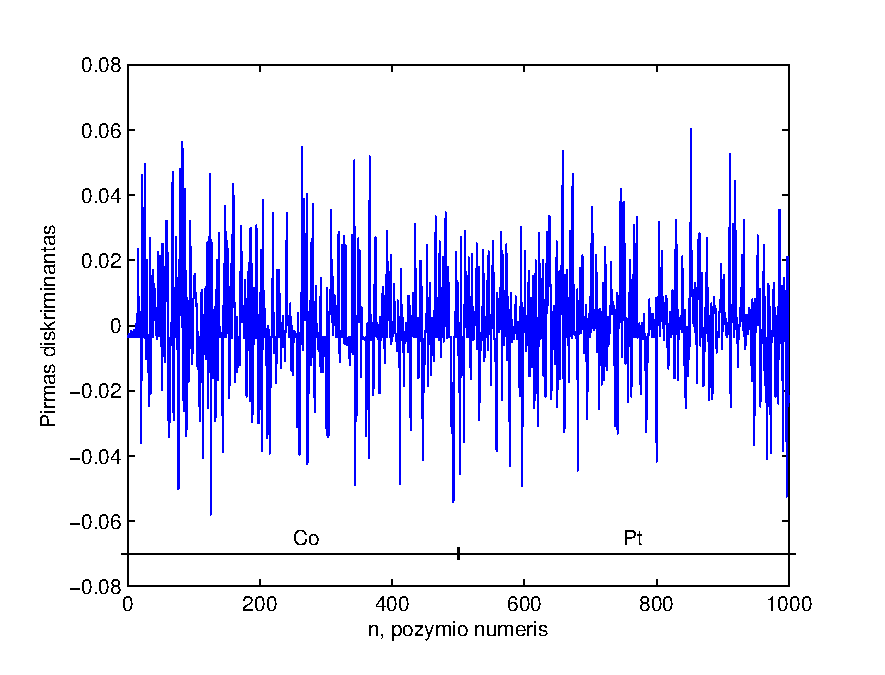
\includegraphics[width=250px]{figures/11_sample_testing}
	\caption{Kojos pakilimo ir kojos prisilietimo prie žemės ilgio variacijos kitimas slenkant langui, po transformacijos}
	\label{fig:testing_sample}
\end{figure}

Tokios išvados verčia projektuoti kitą klasifikavimo mechanizmą, kuris duomenis klasifikuotų ne kiekvieną pagal kiekvieną nagrinėjamą požymį, o pagal požymių grupę -- į laikiną atmintį yra rašoma požymio reikšmė, laukiama, kol laikina atmintis užsipildys iki tam tikros $n$ eilės ir iš gautos sekos yra skaičiuojamas vidurkis (vidurkis skaičiuojamas todėl, nes pagal duomenų pasiskirstymą, kuris parodytas \ref{fig:gauss_lda} paveiksle, pasiskirstymų vidurkiai skiriasi, tačiau variacijos lieka tokios pačios) ir apskaičiuota reikšmė naudojama kaip naujas požymis klasifikatoriaus apmokymui, bei tikrinimui. 

Dėl gaunamų duomenų matmenų ir jų mažo kiekio (kuris priklauso nuo laikinos atminties dydžio, į kurią rašomos naudos erdvės vertės), yra panaudotas paprasčiausias Naivaus Bayes klasifikatoriaus mechanizmas. Duomenys nesikartojo jokiam algoritmo modulyje. Viso erdvės sudarymui panaudota $400$ (nuo $1$ iki $400$), apmokymui $500$ (nuo $501$ iki $1000$), testavimui $500$ ($1001$ iki $1500$) reikšmių. Laikinos atminties ilgis pasirinktas $50$ verčių, iš kurių skaičiuojamas vidurkis. Apmokymo metu iš viso $10$ vidurkiai kiekvienai subjektų grupei, testavimo metu iš viso $10$ vidurkiai kiekvienai subjektų grupei. Gauti tikslumo ir atpažinimo rezultatai pateikti \ref{table:classification_results} lentelėje.

\begin{table}
	\centering
	\renewcommand{\arraystretch}{1.3}
	\caption{Klasifikavimo rezultatas, naudojant naivų Bayes klasifikatorių}
	\label{table:classification_results}
	\begin{tabular}{|c|c|c|} \hline
		& Co & Pt \\ \hline
    Tikslumas & 0,800 & 0,800 \\ \hline
    Atpažinimas & 0,714 & 1,000 \\ \hline
	\end{tabular}
\end{table}

Gautas klasifikavimo tikslumas yra $0,800$, kas viršija prieš tai naudotų metodų tikslumą. Pirmos grupės atpažinimas yra $0,714$, antros grupės atpažinimas $1,000$. Detalesnė klasifikavimo mechanizmo veikimo apžvalga yra pateikta Požymių klasifikavimo programos kūrimo poskyryje.

Skyriuje apžvelgta bendra programos struktūrinė schema, aprašytas kiekvienos schemos elemento tikslas ir funkcija. Aptartas pirminio signalo apdorojimo žingsnio svarba ir būtinumas. Svarbiausias skyriaus rezultatas -- jėgos jutiklių signalo požymio radimas, kurio skirtumas tarp kontrolinio ir Parkinsono liga sergančio subjekto, leidžia identifikuoti eisenos sutrikimą. Atlikus erdvės transformacija, pakito požymio duomenų pasiskirstymai ir tai leido atlikti duomenų klasifikavimą. Skyriuje aptarti galimi panaudoti klasifikatoriai, pateiktas kiekvienas jų veikimo rezultatas, išreikštas tikslumu ir atpažinimu. Algoritmo tikslumui ir atpažinimui padidinti nuspręsta panaudoti laikinąją atmintį požymiams saugoti. Toliau apžvelgtas algoritmo įgyvendinimas.

\section{Signalų analizės programos įgyvendinimas}

Šiame skyriuje apžvelgtas programos įgyvendinimas, jos veikimo struktūra. Kiek iš viso programą sudaro modulių, koks būtinas signalo apdorojimo mechanizmas turi būti atliktas pirmiausiai. Ankstesniuose poskyriuose argumentuotai pažvelgti galimi analizės metodai, požymiai ir klasifikatoriai. Visi rezultatai panaudoti projektuojant galutinį sprendimą. Poskyryje \ref{subsec:total_scheme} pateikta bendra programos algoritmo veikimo schema, poskyryje \ref{subsec:class_scheme} pateikta algoritmo klasifikavimo veikimo schema, poskyryje \ref{subsec:total_program} apžvelgta galutinė programa.

\subsection{Bendro programos algoritmo schemos sudarymas}
\label{subsec:total_scheme}

Ankstesniame skyriuje apžvelgta bendra programos veikimo schema. Bendros schemos pavyzdys yra pateiktas \ref{fig:pirmine_programos_schema} paveiksle. Šiame poskyryje patekta detali algoritmo schema ir aptarta kiekviena jo bloko paskirtis, bei jame naudojamas metodas.

Viso programa sudaryta iš trijų modulių:

\begin{itemize}
\item Požymių erdvės sudarymas;
\item Klasifikatoriaus apmokymas;
\item Klasifikatoriaus tikrinimas.
\end{itemize}

\begin{figure}
  \centering
%  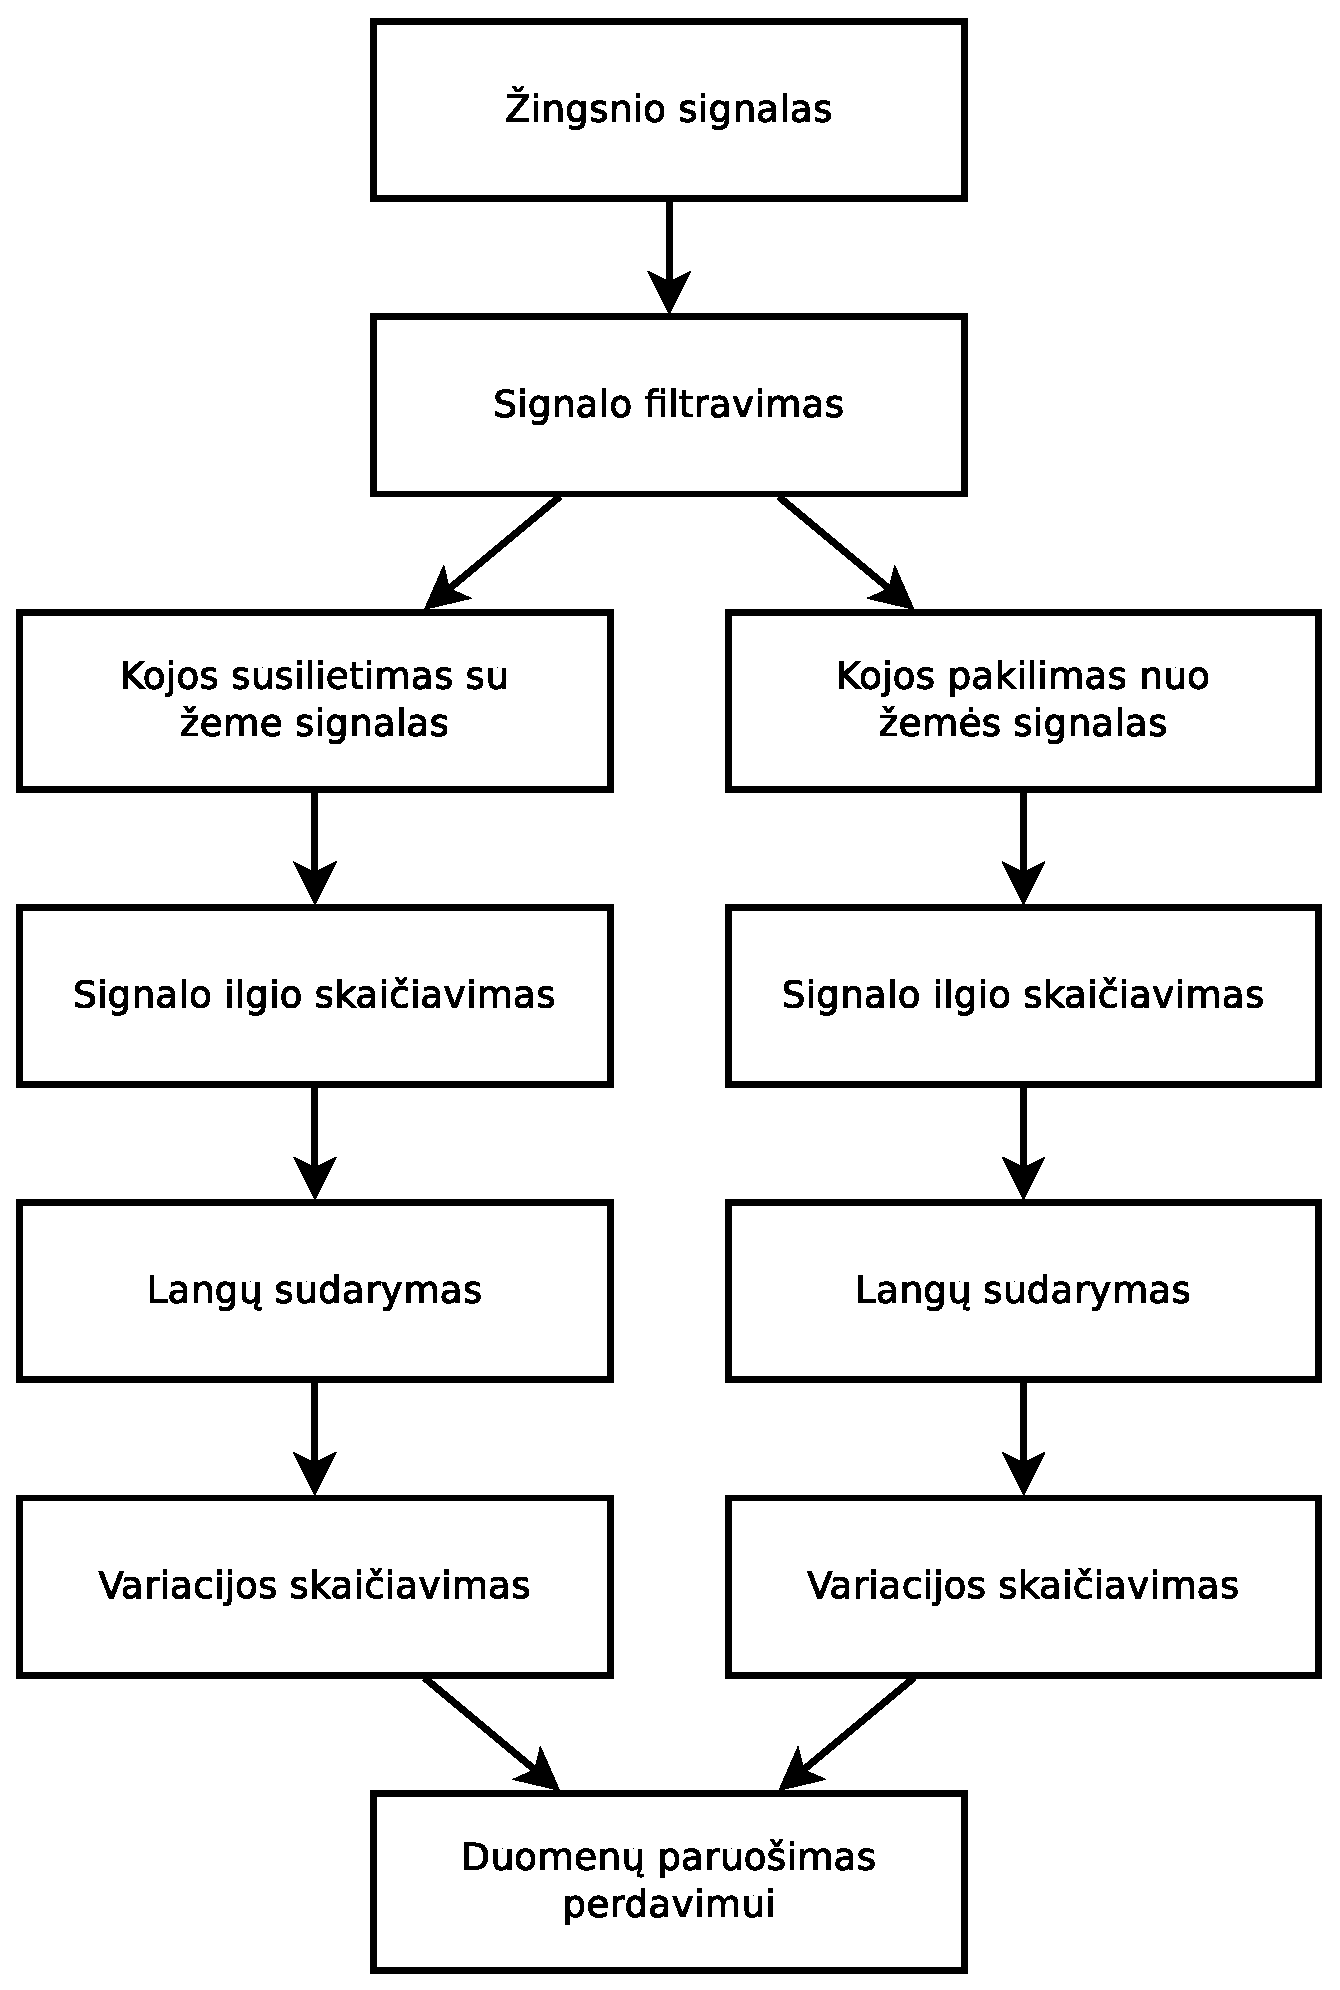
\includegraphics[scale=0.4]{figures/pirminis_signalo_apdorojimas.eps}
  % Graphic for TeX using PGF
% Title: /home/maksim/Documents/Bbd/3_b/figures/pirminis_signalo_apdorojimas.dia
% Creator: Dia v0.97.2
% CreationDate: Thu May 31 00:52:03 2012
% For: maksim
% \usepackage{tikz}
% The following commands are not supported in PSTricks at present
% We define them conditionally, so when they are implemented,
% this pgf file will use them.
\ifx\du\undefined
  \newlength{\du}
\fi
\setlength{\du}{15\unitlength}
\ttfamily\small
\begin{tikzpicture}
\pgftransformxscale{1.000000}
\pgftransformyscale{-1.000000}
\definecolor{dialinecolor}{rgb}{0.000000, 0.000000, 0.000000}
\pgfsetstrokecolor{dialinecolor}
\definecolor{dialinecolor}{rgb}{1.000000, 1.000000, 1.000000}
\pgfsetfillcolor{dialinecolor}
\definecolor{dialinecolor}{rgb}{1.000000, 1.000000, 1.000000}
\pgfsetfillcolor{dialinecolor}
\fill (5.000000\du,9.000000\du)--(5.000000\du,12.000000\du)--(15.000000\du,12.000000\du)--(15.000000\du,9.000000\du)--cycle;
\pgfsetlinewidth{0.100000\du}
\pgfsetdash{}{0pt}
\pgfsetdash{}{0pt}
\pgfsetmiterjoin
\definecolor{dialinecolor}{rgb}{0.000000, 0.000000, 0.000000}
\pgfsetstrokecolor{dialinecolor}
\draw (5.000000\du,9.000000\du)--(5.000000\du,12.000000\du)--(15.000000\du,12.000000\du)--(15.000000\du,9.000000\du)--cycle;
% setfont left to latex
\definecolor{dialinecolor}{rgb}{0.000000, 0.000000, 0.000000}
\pgfsetstrokecolor{dialinecolor}
\node at (10.000000\du,10.695000\du){Signalo filtravimas};
\definecolor{dialinecolor}{rgb}{1.000000, 1.000000, 1.000000}
\pgfsetfillcolor{dialinecolor}
\fill (-1.000000\du,14.000000\du)--(-1.000000\du,17.000000\du)--(9.000000\du,17.000000\du)--(9.000000\du,14.000000\du)--cycle;
\pgfsetlinewidth{0.100000\du}
\pgfsetdash{}{0pt}
\pgfsetdash{}{0pt}
\pgfsetmiterjoin
\definecolor{dialinecolor}{rgb}{0.000000, 0.000000, 0.000000}
\pgfsetstrokecolor{dialinecolor}
\draw (-1.000000\du,14.000000\du)--(-1.000000\du,17.000000\du)--(9.000000\du,17.000000\du)--(9.000000\du,14.000000\du)--cycle;
% setfont left to latex
\definecolor{dialinecolor}{rgb}{0.000000, 0.000000, 0.000000}
\pgfsetstrokecolor{dialinecolor}
\node at (4.000000\du,15.295000\du){Kojos susilietimas su};
% setfont left to latex
\definecolor{dialinecolor}{rgb}{0.000000, 0.000000, 0.000000}
\pgfsetstrokecolor{dialinecolor}
\node at (4.000000\du,16.095000\du){žeme signalas};
\definecolor{dialinecolor}{rgb}{1.000000, 1.000000, 1.000000}
\pgfsetfillcolor{dialinecolor}
\fill (11.000000\du,14.000000\du)--(11.000000\du,17.000000\du)--(21.000000\du,17.000000\du)--(21.000000\du,14.000000\du)--cycle;
\pgfsetlinewidth{0.100000\du}
\pgfsetdash{}{0pt}
\pgfsetdash{}{0pt}
\pgfsetmiterjoin
\definecolor{dialinecolor}{rgb}{0.000000, 0.000000, 0.000000}
\pgfsetstrokecolor{dialinecolor}
\draw (11.000000\du,14.000000\du)--(11.000000\du,17.000000\du)--(21.000000\du,17.000000\du)--(21.000000\du,14.000000\du)--cycle;
% setfont left to latex
\definecolor{dialinecolor}{rgb}{0.000000, 0.000000, 0.000000}
\pgfsetstrokecolor{dialinecolor}
\node at (16.000000\du,15.295000\du){Kojos pakilimas nuo};
% setfont left to latex
\definecolor{dialinecolor}{rgb}{0.000000, 0.000000, 0.000000}
\pgfsetstrokecolor{dialinecolor}
\node at (16.000000\du,16.095000\du){žemės signalas};
\definecolor{dialinecolor}{rgb}{1.000000, 1.000000, 1.000000}
\pgfsetfillcolor{dialinecolor}
\fill (-1.000000\du,19.000000\du)--(-1.000000\du,22.000000\du)--(9.000000\du,22.000000\du)--(9.000000\du,19.000000\du)--cycle;
\pgfsetlinewidth{0.100000\du}
\pgfsetdash{}{0pt}
\pgfsetdash{}{0pt}
\pgfsetmiterjoin
\definecolor{dialinecolor}{rgb}{0.000000, 0.000000, 0.000000}
\pgfsetstrokecolor{dialinecolor}
\draw (-1.000000\du,19.000000\du)--(-1.000000\du,22.000000\du)--(9.000000\du,22.000000\du)--(9.000000\du,19.000000\du)--cycle;
% setfont left to latex
\definecolor{dialinecolor}{rgb}{0.000000, 0.000000, 0.000000}
\pgfsetstrokecolor{dialinecolor}
\node at (4.000000\du,20.695000\du){Signalo ilgio skaičiavimas};
\definecolor{dialinecolor}{rgb}{1.000000, 1.000000, 1.000000}
\pgfsetfillcolor{dialinecolor}
\fill (11.000000\du,19.000000\du)--(11.000000\du,22.000000\du)--(21.000000\du,22.000000\du)--(21.000000\du,19.000000\du)--cycle;
\pgfsetlinewidth{0.100000\du}
\pgfsetdash{}{0pt}
\pgfsetdash{}{0pt}
\pgfsetmiterjoin
\definecolor{dialinecolor}{rgb}{0.000000, 0.000000, 0.000000}
\pgfsetstrokecolor{dialinecolor}
\draw (11.000000\du,19.000000\du)--(11.000000\du,22.000000\du)--(21.000000\du,22.000000\du)--(21.000000\du,19.000000\du)--cycle;
% setfont left to latex
\definecolor{dialinecolor}{rgb}{0.000000, 0.000000, 0.000000}
\pgfsetstrokecolor{dialinecolor}
\node at (16.000000\du,20.695000\du){Signalo ilgio skaičiavimas};
\definecolor{dialinecolor}{rgb}{1.000000, 1.000000, 1.000000}
\pgfsetfillcolor{dialinecolor}
\fill (-1.000000\du,24.000000\du)--(-1.000000\du,27.000000\du)--(9.000000\du,27.000000\du)--(9.000000\du,24.000000\du)--cycle;
\pgfsetlinewidth{0.100000\du}
\pgfsetdash{}{0pt}
\pgfsetdash{}{0pt}
\pgfsetmiterjoin
\definecolor{dialinecolor}{rgb}{0.000000, 0.000000, 0.000000}
\pgfsetstrokecolor{dialinecolor}
\draw (-1.000000\du,24.000000\du)--(-1.000000\du,27.000000\du)--(9.000000\du,27.000000\du)--(9.000000\du,24.000000\du)--cycle;
% setfont left to latex
\definecolor{dialinecolor}{rgb}{0.000000, 0.000000, 0.000000}
\pgfsetstrokecolor{dialinecolor}
\node at (4.000000\du,25.695000\du){Langų sudarymas};
\definecolor{dialinecolor}{rgb}{1.000000, 1.000000, 1.000000}
\pgfsetfillcolor{dialinecolor}
\fill (11.000000\du,24.000000\du)--(11.000000\du,27.000000\du)--(21.000000\du,27.000000\du)--(21.000000\du,24.000000\du)--cycle;
\pgfsetlinewidth{0.100000\du}
\pgfsetdash{}{0pt}
\pgfsetdash{}{0pt}
\pgfsetmiterjoin
\definecolor{dialinecolor}{rgb}{0.000000, 0.000000, 0.000000}
\pgfsetstrokecolor{dialinecolor}
\draw (11.000000\du,24.000000\du)--(11.000000\du,27.000000\du)--(21.000000\du,27.000000\du)--(21.000000\du,24.000000\du)--cycle;
% setfont left to latex
\definecolor{dialinecolor}{rgb}{0.000000, 0.000000, 0.000000}
\pgfsetstrokecolor{dialinecolor}
\node at (16.000000\du,25.695000\du){Langų sudarymas};
\definecolor{dialinecolor}{rgb}{1.000000, 1.000000, 1.000000}
\pgfsetfillcolor{dialinecolor}
\fill (-1.000000\du,29.000000\du)--(-1.000000\du,32.000000\du)--(9.000000\du,32.000000\du)--(9.000000\du,29.000000\du)--cycle;
\pgfsetlinewidth{0.100000\du}
\pgfsetdash{}{0pt}
\pgfsetdash{}{0pt}
\pgfsetmiterjoin
\definecolor{dialinecolor}{rgb}{0.000000, 0.000000, 0.000000}
\pgfsetstrokecolor{dialinecolor}
\draw (-1.000000\du,29.000000\du)--(-1.000000\du,32.000000\du)--(9.000000\du,32.000000\du)--(9.000000\du,29.000000\du)--cycle;
% setfont left to latex
\definecolor{dialinecolor}{rgb}{0.000000, 0.000000, 0.000000}
\pgfsetstrokecolor{dialinecolor}
\node at (4.000000\du,30.695000\du){Variacijos skaičiavimas};
\definecolor{dialinecolor}{rgb}{1.000000, 1.000000, 1.000000}
\pgfsetfillcolor{dialinecolor}
\fill (11.000000\du,29.000000\du)--(11.000000\du,32.000000\du)--(21.000000\du,32.000000\du)--(21.000000\du,29.000000\du)--cycle;
\pgfsetlinewidth{0.100000\du}
\pgfsetdash{}{0pt}
\pgfsetdash{}{0pt}
\pgfsetmiterjoin
\definecolor{dialinecolor}{rgb}{0.000000, 0.000000, 0.000000}
\pgfsetstrokecolor{dialinecolor}
\draw (11.000000\du,29.000000\du)--(11.000000\du,32.000000\du)--(21.000000\du,32.000000\du)--(21.000000\du,29.000000\du)--cycle;
% setfont left to latex
\definecolor{dialinecolor}{rgb}{0.000000, 0.000000, 0.000000}
\pgfsetstrokecolor{dialinecolor}
\node at (16.000000\du,30.695000\du){Variacijos skaičiavimas};
\definecolor{dialinecolor}{rgb}{1.000000, 1.000000, 1.000000}
\pgfsetfillcolor{dialinecolor}
\fill (5.000000\du,34.000000\du)--(5.000000\du,37.000000\du)--(15.000000\du,37.000000\du)--(15.000000\du,34.000000\du)--cycle;
\pgfsetlinewidth{0.100000\du}
\pgfsetdash{}{0pt}
\pgfsetdash{}{0pt}
\pgfsetmiterjoin
\definecolor{dialinecolor}{rgb}{0.000000, 0.000000, 0.000000}
\pgfsetstrokecolor{dialinecolor}
\draw (5.000000\du,34.000000\du)--(5.000000\du,37.000000\du)--(15.000000\du,37.000000\du)--(15.000000\du,34.000000\du)--cycle;
% setfont left to latex
\definecolor{dialinecolor}{rgb}{0.000000, 0.000000, 0.000000}
\pgfsetstrokecolor{dialinecolor}
\node at (10.000000\du,35.295000\du){Duomenų paruošimas};
% setfont left to latex
\definecolor{dialinecolor}{rgb}{0.000000, 0.000000, 0.000000}
\pgfsetstrokecolor{dialinecolor}
\node at (10.000000\du,36.095000\du){perdavimui};
\pgfsetlinewidth{0.100000\du}
\pgfsetdash{}{0pt}
\pgfsetdash{}{0pt}
\pgfsetbuttcap
{
\definecolor{dialinecolor}{rgb}{0.000000, 0.000000, 0.000000}
\pgfsetfillcolor{dialinecolor}
% was here!!!
\pgfsetarrowsend{stealth}
\definecolor{dialinecolor}{rgb}{0.000000, 0.000000, 0.000000}
\pgfsetstrokecolor{dialinecolor}
\draw (8.141113\du,12.049072\du)--(5.858887\du,13.950928\du);
}
\pgfsetlinewidth{0.100000\du}
\pgfsetdash{}{0pt}
\pgfsetdash{}{0pt}
\pgfsetbuttcap
{
\definecolor{dialinecolor}{rgb}{0.000000, 0.000000, 0.000000}
\pgfsetfillcolor{dialinecolor}
% was here!!!
\pgfsetarrowsend{stealth}
\definecolor{dialinecolor}{rgb}{0.000000, 0.000000, 0.000000}
\pgfsetstrokecolor{dialinecolor}
\draw (11.858887\du,12.049072\du)--(14.141113\du,13.950928\du);
}
\pgfsetlinewidth{0.100000\du}
\pgfsetdash{}{0pt}
\pgfsetdash{}{0pt}
\pgfsetbuttcap
{
\definecolor{dialinecolor}{rgb}{0.000000, 0.000000, 0.000000}
\pgfsetfillcolor{dialinecolor}
% was here!!!
\pgfsetarrowsend{stealth}
\definecolor{dialinecolor}{rgb}{0.000000, 0.000000, 0.000000}
\pgfsetstrokecolor{dialinecolor}
\draw (4.000000\du,17.049072\du)--(4.000000\du,18.950928\du);
}
\pgfsetlinewidth{0.100000\du}
\pgfsetdash{}{0pt}
\pgfsetdash{}{0pt}
\pgfsetbuttcap
{
\definecolor{dialinecolor}{rgb}{0.000000, 0.000000, 0.000000}
\pgfsetfillcolor{dialinecolor}
% was here!!!
\pgfsetarrowsend{stealth}
\definecolor{dialinecolor}{rgb}{0.000000, 0.000000, 0.000000}
\pgfsetstrokecolor{dialinecolor}
\draw (16.000000\du,17.049072\du)--(16.000000\du,18.950928\du);
}
\pgfsetlinewidth{0.100000\du}
\pgfsetdash{}{0pt}
\pgfsetdash{}{0pt}
\pgfsetbuttcap
{
\definecolor{dialinecolor}{rgb}{0.000000, 0.000000, 0.000000}
\pgfsetfillcolor{dialinecolor}
% was here!!!
\pgfsetarrowsend{stealth}
\definecolor{dialinecolor}{rgb}{0.000000, 0.000000, 0.000000}
\pgfsetstrokecolor{dialinecolor}
\draw (16.000000\du,22.049072\du)--(16.000000\du,23.950928\du);
}
\pgfsetlinewidth{0.100000\du}
\pgfsetdash{}{0pt}
\pgfsetdash{}{0pt}
\pgfsetbuttcap
{
\definecolor{dialinecolor}{rgb}{0.000000, 0.000000, 0.000000}
\pgfsetfillcolor{dialinecolor}
% was here!!!
\pgfsetarrowsend{stealth}
\definecolor{dialinecolor}{rgb}{0.000000, 0.000000, 0.000000}
\pgfsetstrokecolor{dialinecolor}
\draw (16.000000\du,27.049072\du)--(16.000000\du,28.950928\du);
}
\pgfsetlinewidth{0.100000\du}
\pgfsetdash{}{0pt}
\pgfsetdash{}{0pt}
\pgfsetbuttcap
{
\definecolor{dialinecolor}{rgb}{0.000000, 0.000000, 0.000000}
\pgfsetfillcolor{dialinecolor}
% was here!!!
\pgfsetarrowsend{stealth}
\definecolor{dialinecolor}{rgb}{0.000000, 0.000000, 0.000000}
\pgfsetstrokecolor{dialinecolor}
\draw (14.141113\du,32.049072\du)--(11.858887\du,33.950928\du);
}
\pgfsetlinewidth{0.100000\du}
\pgfsetdash{}{0pt}
\pgfsetdash{}{0pt}
\pgfsetbuttcap
{
\definecolor{dialinecolor}{rgb}{0.000000, 0.000000, 0.000000}
\pgfsetfillcolor{dialinecolor}
% was here!!!
\pgfsetarrowsend{stealth}
\definecolor{dialinecolor}{rgb}{0.000000, 0.000000, 0.000000}
\pgfsetstrokecolor{dialinecolor}
\draw (4.000000\du,22.049072\du)--(4.000000\du,23.950928\du);
}
\pgfsetlinewidth{0.100000\du}
\pgfsetdash{}{0pt}
\pgfsetdash{}{0pt}
\pgfsetbuttcap
{
\definecolor{dialinecolor}{rgb}{0.000000, 0.000000, 0.000000}
\pgfsetfillcolor{dialinecolor}
% was here!!!
\pgfsetarrowsend{stealth}
\definecolor{dialinecolor}{rgb}{0.000000, 0.000000, 0.000000}
\pgfsetstrokecolor{dialinecolor}
\draw (4.000000\du,27.049072\du)--(4.000000\du,28.950928\du);
}
\pgfsetlinewidth{0.100000\du}
\pgfsetdash{}{0pt}
\pgfsetdash{}{0pt}
\pgfsetbuttcap
{
\definecolor{dialinecolor}{rgb}{0.000000, 0.000000, 0.000000}
\pgfsetfillcolor{dialinecolor}
% was here!!!
\pgfsetarrowsend{stealth}
\definecolor{dialinecolor}{rgb}{0.000000, 0.000000, 0.000000}
\pgfsetstrokecolor{dialinecolor}
\draw (5.858887\du,32.049072\du)--(8.141113\du,33.950928\du);
}
\definecolor{dialinecolor}{rgb}{1.000000, 1.000000, 1.000000}
\pgfsetfillcolor{dialinecolor}
\fill (5.000000\du,4.000000\du)--(5.000000\du,7.000000\du)--(15.000000\du,7.000000\du)--(15.000000\du,4.000000\du)--cycle;
\pgfsetlinewidth{0.100000\du}
\pgfsetdash{}{0pt}
\pgfsetdash{}{0pt}
\pgfsetmiterjoin
\definecolor{dialinecolor}{rgb}{0.000000, 0.000000, 0.000000}
\pgfsetstrokecolor{dialinecolor}
\draw (5.000000\du,4.000000\du)--(5.000000\du,7.000000\du)--(15.000000\du,7.000000\du)--(15.000000\du,4.000000\du)--cycle;
% setfont left to latex
\definecolor{dialinecolor}{rgb}{0.000000, 0.000000, 0.000000}
\pgfsetstrokecolor{dialinecolor}
\node at (10.000000\du,5.695000\du){Žingsnio signalas};
\pgfsetlinewidth{0.100000\du}
\pgfsetdash{}{0pt}
\pgfsetdash{}{0pt}
\pgfsetbuttcap
{
\definecolor{dialinecolor}{rgb}{0.000000, 0.000000, 0.000000}
\pgfsetfillcolor{dialinecolor}
% was here!!!
\pgfsetarrowsend{stealth}
\definecolor{dialinecolor}{rgb}{0.000000, 0.000000, 0.000000}
\pgfsetstrokecolor{dialinecolor}
\draw (10.000000\du,7.049072\du)--(10.000000\du,8.950928\du);
}
\end{tikzpicture}

  \caption{Pirminio signalo apdorojimo schema}
  \label{fig:pre_phase}
\end{figure}

\begin{cfigure}[b]
  \centering
  \caption{Signalo filtravimas dviem Butterworth filtrais}
  \label{code:filter}
  \begin{lstlisting}
    [B,A] = butter(9, 1/50, 'high');
    [BB,AA] = butter(9, 40/50, 'low');
    output = filter(BB, AA, filter(B, A, input));
  \end{lstlisting}
\end{cfigure}

Kiekvieno modulio pradžioje yra vykdomas pirminio signalo apdorojimas pagal schemą, pavaizduota \ref{fig:pre_phase} paveiksle. Pirminis bloko uždavinys yra nereikalingų dažninių komponenčių pašalinimas. Matlab aplinkoje signalo filtravimas yra atliekamas $9$ eilės \textit{Butterworth} filtru. Kodas pateiktas \ref{code:filter} programiniam kode. Pirmasis, aukštų dažnių filtras, skirtas pašalinti signalo nuolatinei komponentei. Antras, žemų dažnių filtras, skirtas pašalinti aukšto dažnio triukšmą, kuris neneša visiškai jokios naudingos informacijos. Abiejų filtrų eilė yra 9-ta, žemų dažnių filtro ribinis dažnis parinktas $40$ Hz. Duomenys diskretizuojami $100$ Hz dažniu, vadinasi didžiausias galimas signalo dažnis yra $50$ Hz. Didžiausias žmogaus generuojamas dažnis ėjimo metu, remiantis šaltiniu, yra $20$ Hz. Užtikrintumui parinktas $40$ Hz dažnis. Nuolatinė dedamoji pašalinama su aukšto dažnio filtru, kurio ribinis dažnis yra $1$ Hz. Nuolatinė dedamoji neneša jokios informacijos apie eiseną, kadangi ji tiktai nurodo naudojamų jutiklių jautrumą.

\begin{cfigure}
  \centering
  \caption{Kontakto su žeme signalo išskyrimo programos kodo fragmentas}
  \label{code:signal_extraction}
  \lstinputlisting{sources/extract_signal.m}
\end{cfigure}

\begin{figure}
  \centering
  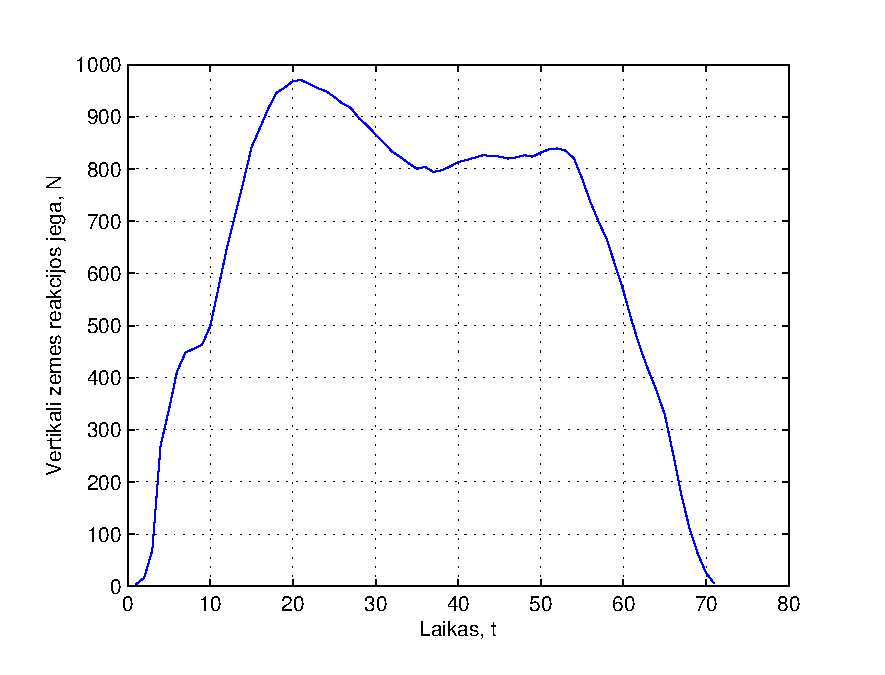
\includegraphics[width=300px]{figures/09_sample_stance_phase.eps}
  \caption{Susilietimo su žeme signalas}
  \label{fig:stance_phase}
\end{figure}

Signalo skirstymas pagal žinomą fizinę veiklą Matlab aplinkoje įgyvendintas kodo fragmentas yra pateikiamas \ref{code:signal_extraction} programiniam kode. Pirmiausiai, ``Pt\_t'' kintamojo struktūroje yra saugomi kairės kojos Parkinsono liga sergančių subjektų duomenys. Kiekvienas signalas yra priskiriamas prie $signal$ kintamojo, su kuriuo toliau yra tęsiamas apdorojimo procesas. Jeigu signalas nėra lygus nuliui, tuomet jis įdedamas į laikinąją atmintį. Taip signalas yra tikrinamas iki tol, kol signalas tampa lygus nuliui ir tęsiamas tolimesnis apdorojimas. Apdorojimas susideda iš signalo ilgio patikros. Jeigu signalas yra trumpesnis už 10 verčių, arba turint omenyje, kad signalas diskretizuojamas $100$ Hz, tai $0,1$ s, vadinasi, signalas yra tiesiog aukšto dažnio triukšmas arba blogas pavyzdys ir signalas yra atmetamas. Jeigu signalas yra ilgesnis už 200 verčių ($2$ s), vadinasi, duomenų rinkimo metu įvyko klaida ir koja per tokį laiką nebuvo pakelta. Tokia klaida gali būti sukelta, kuomet subjektas ne eina, o stovi ant dviejų kojų arba tik ant kairės kojos. Jeigu visi kriterijai patenkinami, signalas yra priimamas ir kraunamas į laikinąją atmintį, pavadinimu ``$data.Pt$''. Signalas, kuriuo metu koja neliečia žemės, yra randamas kartu su ankščiau išnagrinėtu metu. Algoritmas patikrina kiek praėjo laiko (arba kiek verčių yra priskaičiuota) nuo paskutinio užskaityto kojos ant žemės signalo ir įrašo tą signalą į laikiną atmintį, jeigu po praeito signalo nepraėjo mažiau negu 50 verčių arba $0,5$ s ir nedaugiau nei 200 verčių arba $2$ s. Signalas pavaizduotas \ref{fig:stance_phase} paveiksle.

\begin{figure}
  \centering
%  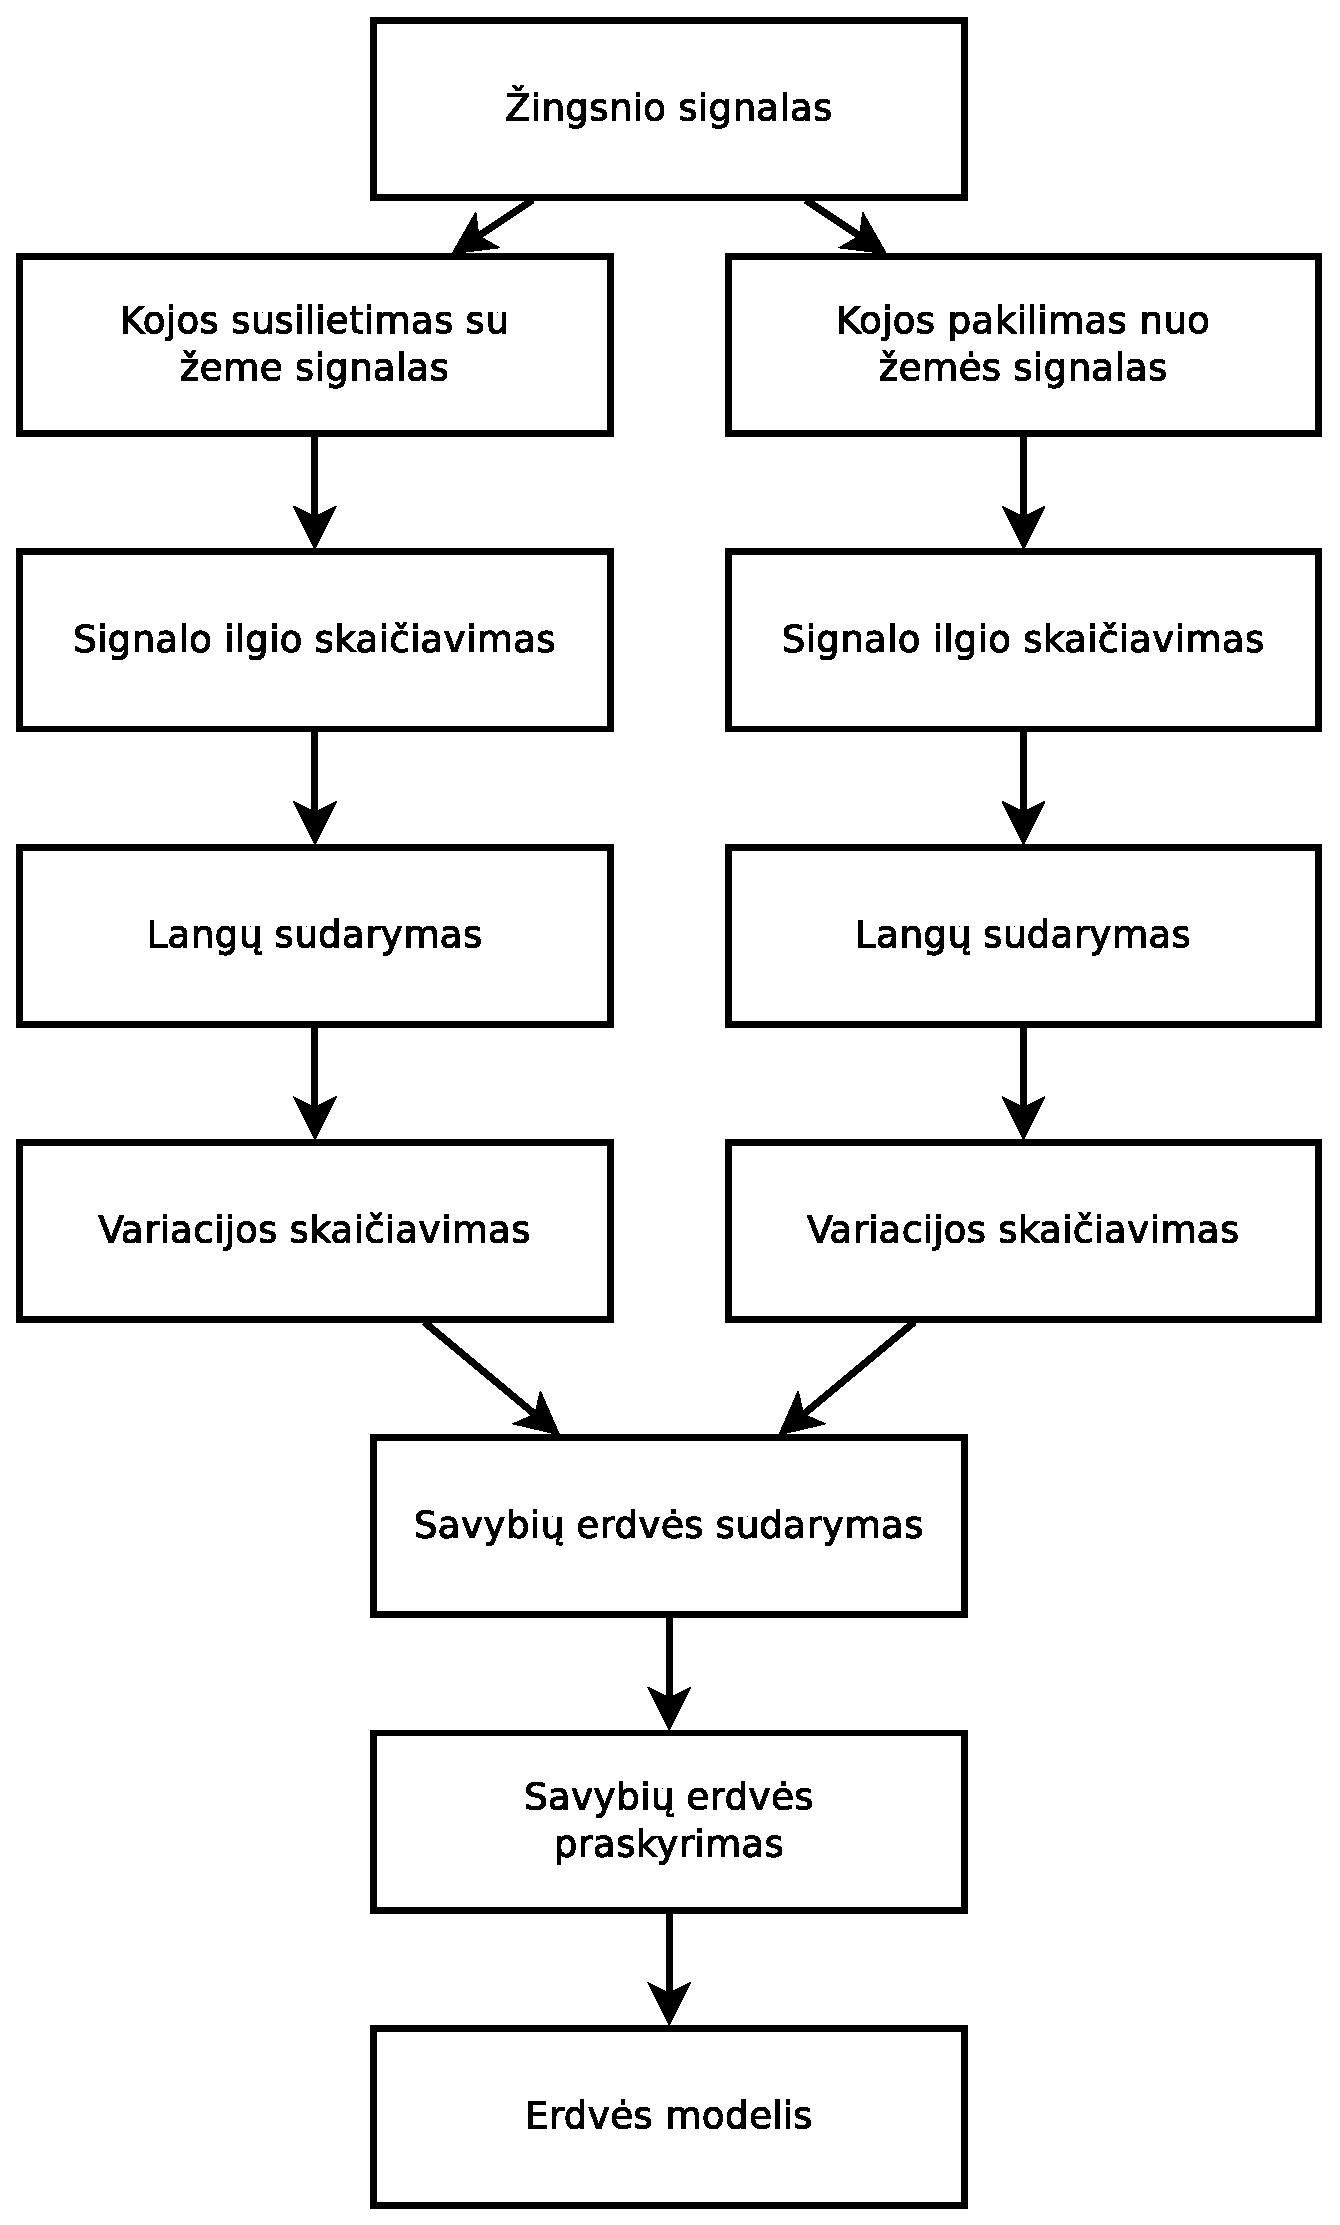
\includegraphics[scale=0.5]{figures/pirma_faze.eps}
  % Graphic for TeX using PGF
% Title: /home/maksim/Documents/Bbd/3_b/figures/pirma_faze.dia
% Creator: Dia v0.97.2
% CreationDate: Thu May 31 00:51:14 2012
% For: maksim
% \usepackage{tikz}
% The following commands are not supported in PSTricks at present
% We define them conditionally, so when they are implemented,
% this pgf file will use them.
\ifx\du\undefined
  \newlength{\du}
\fi
\setlength{\du}{15\unitlength}
\ttfamily\small
\begin{tikzpicture}
\pgftransformxscale{1.000000}
\pgftransformyscale{-1.000000}
\definecolor{dialinecolor}{rgb}{0.000000, 0.000000, 0.000000}
\pgfsetstrokecolor{dialinecolor}
\definecolor{dialinecolor}{rgb}{1.000000, 1.000000, 1.000000}
\pgfsetfillcolor{dialinecolor}
\definecolor{dialinecolor}{rgb}{1.000000, 1.000000, 1.000000}
\pgfsetfillcolor{dialinecolor}
\fill (5.000000\du,34.000000\du)--(5.000000\du,37.000000\du)--(15.000000\du,37.000000\du)--(15.000000\du,34.000000\du)--cycle;
\pgfsetlinewidth{0.100000\du}
\pgfsetdash{}{0pt}
\pgfsetdash{}{0pt}
\pgfsetmiterjoin
\definecolor{dialinecolor}{rgb}{0.000000, 0.000000, 0.000000}
\pgfsetstrokecolor{dialinecolor}
\draw (5.000000\du,34.000000\du)--(5.000000\du,37.000000\du)--(15.000000\du,37.000000\du)--(15.000000\du,34.000000\du)--cycle;
% setfont left to latex
\definecolor{dialinecolor}{rgb}{0.000000, 0.000000, 0.000000}
\pgfsetstrokecolor{dialinecolor}
\node at (10.000000\du,35.695000\du){Požymių erdvės sudarymas};
\definecolor{dialinecolor}{rgb}{1.000000, 1.000000, 1.000000}
\pgfsetfillcolor{dialinecolor}
\fill (5.000000\du,39.000000\du)--(5.000000\du,42.000000\du)--(15.000000\du,42.000000\du)--(15.000000\du,39.000000\du)--cycle;
\pgfsetlinewidth{0.100000\du}
\pgfsetdash{}{0pt}
\pgfsetdash{}{0pt}
\pgfsetmiterjoin
\definecolor{dialinecolor}{rgb}{0.000000, 0.000000, 0.000000}
\pgfsetstrokecolor{dialinecolor}
\draw (5.000000\du,39.000000\du)--(5.000000\du,42.000000\du)--(15.000000\du,42.000000\du)--(15.000000\du,39.000000\du)--cycle;
% setfont left to latex
\definecolor{dialinecolor}{rgb}{0.000000, 0.000000, 0.000000}
\pgfsetstrokecolor{dialinecolor}
\node at (10.000000\du,40.295000\du){Požymių erdvės};
% setfont left to latex
\definecolor{dialinecolor}{rgb}{0.000000, 0.000000, 0.000000}
\pgfsetstrokecolor{dialinecolor}
\node at (10.000000\du,41.095000\du){praskyrimas};
\pgfsetlinewidth{0.100000\du}
\pgfsetdash{}{0pt}
\pgfsetdash{}{0pt}
\pgfsetbuttcap
{
\definecolor{dialinecolor}{rgb}{0.000000, 0.000000, 0.000000}
\pgfsetfillcolor{dialinecolor}
% was here!!!
\pgfsetarrowsend{stealth}
\definecolor{dialinecolor}{rgb}{0.000000, 0.000000, 0.000000}
\pgfsetstrokecolor{dialinecolor}
\draw (10.000000\du,37.049072\du)--(10.000000\du,38.950928\du);
}
\definecolor{dialinecolor}{rgb}{1.000000, 1.000000, 1.000000}
\pgfsetfillcolor{dialinecolor}
\fill (5.000000\du,44.000000\du)--(5.000000\du,47.000000\du)--(15.000000\du,47.000000\du)--(15.000000\du,44.000000\du)--cycle;
\pgfsetlinewidth{0.100000\du}
\pgfsetdash{}{0pt}
\pgfsetdash{}{0pt}
\pgfsetmiterjoin
\definecolor{dialinecolor}{rgb}{0.000000, 0.000000, 0.000000}
\pgfsetstrokecolor{dialinecolor}
\draw (5.000000\du,44.000000\du)--(5.000000\du,47.000000\du)--(15.000000\du,47.000000\du)--(15.000000\du,44.000000\du)--cycle;
% setfont left to latex
\definecolor{dialinecolor}{rgb}{0.000000, 0.000000, 0.000000}
\pgfsetstrokecolor{dialinecolor}
\node at (10.000000\du,45.695000\du){Erdvės modelis};
\pgfsetlinewidth{0.100000\du}
\pgfsetdash{}{0pt}
\pgfsetdash{}{0pt}
\pgfsetbuttcap
{
\definecolor{dialinecolor}{rgb}{0.000000, 0.000000, 0.000000}
\pgfsetfillcolor{dialinecolor}
% was here!!!
\pgfsetarrowsend{stealth}
\definecolor{dialinecolor}{rgb}{0.000000, 0.000000, 0.000000}
\pgfsetstrokecolor{dialinecolor}
\draw (10.000000\du,42.049072\du)--(10.000000\du,43.950928\du);
}
\pgfsetlinewidth{0.100000\du}
\pgfsetdash{}{0pt}
\pgfsetdash{}{0pt}
\pgfsetbuttcap
{
\definecolor{dialinecolor}{rgb}{0.000000, 0.000000, 0.000000}
\pgfsetfillcolor{dialinecolor}
% was here!!!
\pgfsetarrowsend{stealth}
\definecolor{dialinecolor}{rgb}{0.000000, 0.000000, 0.000000}
\pgfsetstrokecolor{dialinecolor}
\draw (10.000000\du,32.049072\du)--(10.000000\du,33.950928\du);
}
\definecolor{dialinecolor}{rgb}{1.000000, 1.000000, 1.000000}
\pgfsetfillcolor{dialinecolor}
\fill (5.000000\du,29.000000\du)--(5.000000\du,32.000000\du)--(15.000000\du,32.000000\du)--(15.000000\du,29.000000\du)--cycle;
\pgfsetlinewidth{0.100000\du}
\pgfsetdash{}{0pt}
\pgfsetdash{}{0pt}
\pgfsetmiterjoin
\definecolor{dialinecolor}{rgb}{0.000000, 0.000000, 0.000000}
\pgfsetstrokecolor{dialinecolor}
\draw (5.000000\du,29.000000\du)--(5.000000\du,32.000000\du)--(15.000000\du,32.000000\du)--(15.000000\du,29.000000\du)--cycle;
% setfont left to latex
\definecolor{dialinecolor}{rgb}{0.000000, 0.000000, 0.000000}
\pgfsetstrokecolor{dialinecolor}
\node at (10.000000\du,30.295000\du){Pirminis signalo};
% setfont left to latex
\definecolor{dialinecolor}{rgb}{0.000000, 0.000000, 0.000000}
\pgfsetstrokecolor{dialinecolor}
\node at (10.000000\du,31.095000\du){apdorojimas};
\end{tikzpicture}

  \caption{Programos pirmo modulio, požymių erdvės sudarymo, veikimo schema}
  \label{fig:pirma_faze}
\end{figure}

Programos pirmo modulio struktūrinė schema atvaizduota \ref{fig:pirma_faze} paveiksle. Modulis iš pirminio signalo apdorojimo nuskaito variacijos skaičiavimus, tuomet iš dviejų matmenų požymių sudaro požymių erdvę, pritaiko LDA transformaciją su Gauso branduoliu. Rezultate programa gražina erdvės modelį, kuris susideda iš tikrinio vektoriaus ir duomenų vidurkio.


\begin{figure}
  \centering
%  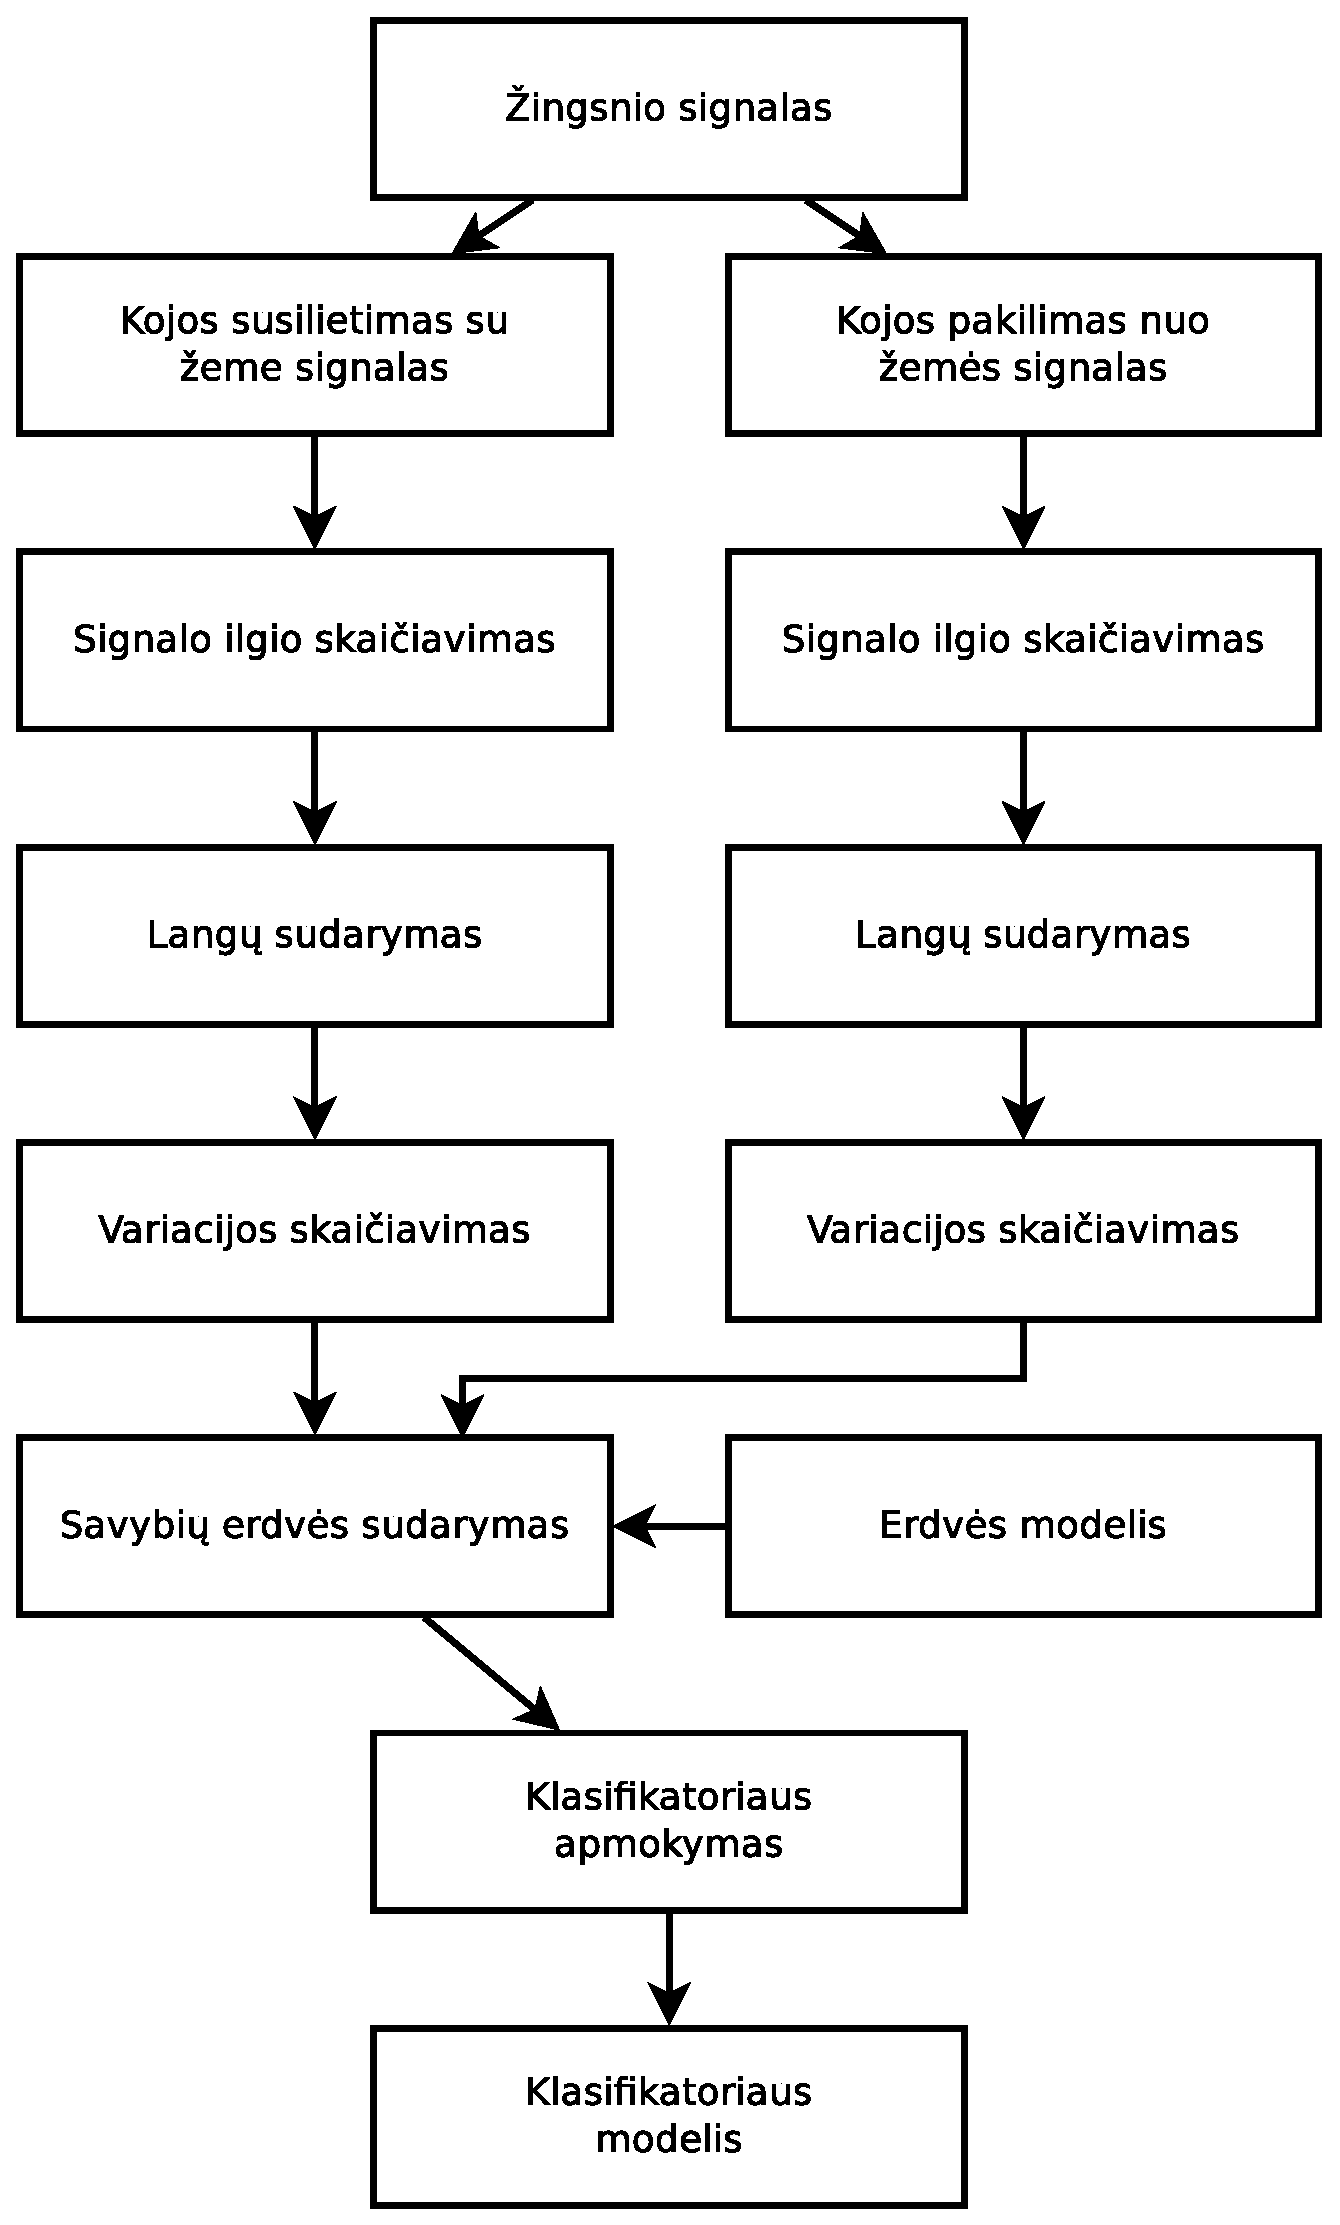
\includegraphics[scale=0.5]{figures/antra_faze.eps}
  % Graphic for TeX using PGF
% Title: /home/maksim/Documents/Bbd/3_b/figures/antra_faze.dia
% Creator: Dia v0.97.2
% CreationDate: Thu May 31 00:45:02 2012
% For: maksim
% \usepackage{tikz}
% The following commands are not supported in PSTricks at present
% We define them conditionally, so when they are implemented,
% this pgf file will use them.
\ifx\du\undefined
  \newlength{\du}
\fi
\setlength{\du}{15\unitlength}
\ttfamily\small
\begin{tikzpicture}
\pgftransformxscale{1.000000}
\pgftransformyscale{-1.000000}
\definecolor{dialinecolor}{rgb}{0.000000, 0.000000, 0.000000}
\pgfsetstrokecolor{dialinecolor}
\definecolor{dialinecolor}{rgb}{1.000000, 1.000000, 1.000000}
\pgfsetfillcolor{dialinecolor}
\definecolor{dialinecolor}{rgb}{1.000000, 1.000000, 1.000000}
\pgfsetfillcolor{dialinecolor}
\fill (-1.000000\du,34.000000\du)--(-1.000000\du,37.000000\du)--(9.000000\du,37.000000\du)--(9.000000\du,34.000000\du)--cycle;
\pgfsetlinewidth{0.100000\du}
\pgfsetdash{}{0pt}
\pgfsetdash{}{0pt}
\pgfsetmiterjoin
\definecolor{dialinecolor}{rgb}{0.000000, 0.000000, 0.000000}
\pgfsetstrokecolor{dialinecolor}
\draw (-1.000000\du,34.000000\du)--(-1.000000\du,37.000000\du)--(9.000000\du,37.000000\du)--(9.000000\du,34.000000\du)--cycle;
% setfont left to latex
\definecolor{dialinecolor}{rgb}{0.000000, 0.000000, 0.000000}
\pgfsetstrokecolor{dialinecolor}
\node at (4.000000\du,35.695000\du){Požymių erdvės sudarymas};
\pgfsetlinewidth{0.100000\du}
\pgfsetdash{}{0pt}
\pgfsetdash{}{0pt}
\pgfsetbuttcap
{
\definecolor{dialinecolor}{rgb}{0.000000, 0.000000, 0.000000}
\pgfsetfillcolor{dialinecolor}
% was here!!!
\pgfsetarrowsend{stealth}
\definecolor{dialinecolor}{rgb}{0.000000, 0.000000, 0.000000}
\pgfsetstrokecolor{dialinecolor}
\draw (8.141113\du,32.049072\du)--(5.858887\du,33.950928\du);
}
\definecolor{dialinecolor}{rgb}{1.000000, 1.000000, 1.000000}
\pgfsetfillcolor{dialinecolor}
\fill (11.000000\du,34.000000\du)--(11.000000\du,37.000000\du)--(21.000000\du,37.000000\du)--(21.000000\du,34.000000\du)--cycle;
\pgfsetlinewidth{0.100000\du}
\pgfsetdash{}{0pt}
\pgfsetdash{}{0pt}
\pgfsetmiterjoin
\definecolor{dialinecolor}{rgb}{0.000000, 0.000000, 0.000000}
\pgfsetstrokecolor{dialinecolor}
\draw (11.000000\du,34.000000\du)--(11.000000\du,37.000000\du)--(21.000000\du,37.000000\du)--(21.000000\du,34.000000\du)--cycle;
% setfont left to latex
\definecolor{dialinecolor}{rgb}{0.000000, 0.000000, 0.000000}
\pgfsetstrokecolor{dialinecolor}
\node at (16.000000\du,35.695000\du){Erdvės modelis};
\pgfsetlinewidth{0.100000\du}
\pgfsetdash{}{0pt}
\pgfsetdash{}{0pt}
\pgfsetbuttcap
{
\definecolor{dialinecolor}{rgb}{0.000000, 0.000000, 0.000000}
\pgfsetfillcolor{dialinecolor}
% was here!!!
\pgfsetarrowsend{stealth}
\definecolor{dialinecolor}{rgb}{0.000000, 0.000000, 0.000000}
\pgfsetstrokecolor{dialinecolor}
\draw (10.955078\du,35.500000\du)--(9.044922\du,35.500000\du);
}
\definecolor{dialinecolor}{rgb}{1.000000, 1.000000, 1.000000}
\pgfsetfillcolor{dialinecolor}
\fill (5.000000\du,39.000000\du)--(5.000000\du,42.000000\du)--(15.000000\du,42.000000\du)--(15.000000\du,39.000000\du)--cycle;
\pgfsetlinewidth{0.100000\du}
\pgfsetdash{}{0pt}
\pgfsetdash{}{0pt}
\pgfsetmiterjoin
\definecolor{dialinecolor}{rgb}{0.000000, 0.000000, 0.000000}
\pgfsetstrokecolor{dialinecolor}
\draw (5.000000\du,39.000000\du)--(5.000000\du,42.000000\du)--(15.000000\du,42.000000\du)--(15.000000\du,39.000000\du)--cycle;
% setfont left to latex
\definecolor{dialinecolor}{rgb}{0.000000, 0.000000, 0.000000}
\pgfsetstrokecolor{dialinecolor}
\node at (10.000000\du,40.295000\du){Klasifikatoriaus};
% setfont left to latex
\definecolor{dialinecolor}{rgb}{0.000000, 0.000000, 0.000000}
\pgfsetstrokecolor{dialinecolor}
\node at (10.000000\du,41.095000\du){apmokymas};
\pgfsetlinewidth{0.100000\du}
\pgfsetdash{}{0pt}
\pgfsetdash{}{0pt}
\pgfsetbuttcap
{
\definecolor{dialinecolor}{rgb}{0.000000, 0.000000, 0.000000}
\pgfsetfillcolor{dialinecolor}
% was here!!!
\pgfsetarrowsend{stealth}
\definecolor{dialinecolor}{rgb}{0.000000, 0.000000, 0.000000}
\pgfsetstrokecolor{dialinecolor}
\draw (5.858887\du,37.049072\du)--(8.141113\du,38.950928\du);
}
\definecolor{dialinecolor}{rgb}{1.000000, 1.000000, 1.000000}
\pgfsetfillcolor{dialinecolor}
\fill (5.000000\du,44.000000\du)--(5.000000\du,47.000000\du)--(15.000000\du,47.000000\du)--(15.000000\du,44.000000\du)--cycle;
\pgfsetlinewidth{0.100000\du}
\pgfsetdash{}{0pt}
\pgfsetdash{}{0pt}
\pgfsetmiterjoin
\definecolor{dialinecolor}{rgb}{0.000000, 0.000000, 0.000000}
\pgfsetstrokecolor{dialinecolor}
\draw (5.000000\du,44.000000\du)--(5.000000\du,47.000000\du)--(15.000000\du,47.000000\du)--(15.000000\du,44.000000\du)--cycle;
% setfont left to latex
\definecolor{dialinecolor}{rgb}{0.000000, 0.000000, 0.000000}
\pgfsetstrokecolor{dialinecolor}
\node at (10.000000\du,45.295000\du){Klasifikatoriaus};
% setfont left to latex
\definecolor{dialinecolor}{rgb}{0.000000, 0.000000, 0.000000}
\pgfsetstrokecolor{dialinecolor}
\node at (10.000000\du,46.095000\du){modelis};
\pgfsetlinewidth{0.100000\du}
\pgfsetdash{}{0pt}
\pgfsetdash{}{0pt}
\pgfsetbuttcap
{
\definecolor{dialinecolor}{rgb}{0.000000, 0.000000, 0.000000}
\pgfsetfillcolor{dialinecolor}
% was here!!!
\pgfsetarrowsend{stealth}
\definecolor{dialinecolor}{rgb}{0.000000, 0.000000, 0.000000}
\pgfsetstrokecolor{dialinecolor}
\draw (10.000000\du,42.049072\du)--(10.000000\du,43.950928\du);
}
\definecolor{dialinecolor}{rgb}{1.000000, 1.000000, 1.000000}
\pgfsetfillcolor{dialinecolor}
\fill (5.000000\du,29.000000\du)--(5.000000\du,32.000000\du)--(15.000000\du,32.000000\du)--(15.000000\du,29.000000\du)--cycle;
\pgfsetlinewidth{0.100000\du}
\pgfsetdash{}{0pt}
\pgfsetdash{}{0pt}
\pgfsetmiterjoin
\definecolor{dialinecolor}{rgb}{0.000000, 0.000000, 0.000000}
\pgfsetstrokecolor{dialinecolor}
\draw (5.000000\du,29.000000\du)--(5.000000\du,32.000000\du)--(15.000000\du,32.000000\du)--(15.000000\du,29.000000\du)--cycle;
% setfont left to latex
\definecolor{dialinecolor}{rgb}{0.000000, 0.000000, 0.000000}
\pgfsetstrokecolor{dialinecolor}
\node at (10.000000\du,30.295000\du){Pirminis signalo};
% setfont left to latex
\definecolor{dialinecolor}{rgb}{0.000000, 0.000000, 0.000000}
\pgfsetstrokecolor{dialinecolor}
\node at (10.000000\du,31.095000\du){apdorojimas};
\end{tikzpicture}

  \caption{Antro modulio, klasifikatoriaus apmokymo, veikimo schema}
  \label{fig:antra_faze}
\end{figure}

Programos antro modulio struktūrinė schema atvaizduota \ref{fig:antra_faze} paveiksle. Modulis iš pirminio signalo apdorojimo nuskaito variacijos skaičiavimus. Struktūroje naudojamas erdvės modelis iš pirmojo programos modulio. Jis reikalingas tam, kad kiekvieną kartą neprojektuoti naujos erdvės iš naujo, bet projektuoti naujus duomenis į jau esamą erdvę. Tai taip pat užtikrina, kad naudojama ta pati matmenų erdvė, kas leidžia užtikrinti duomenų apibendrinimą. Skirtumas taip pirmojo ir antrojo modulio yra antro modulio išėjime yra klasifikatoriaus modelis, kuris yra apmokyto klasifikatoriaus parametrai, kurie yra naudojami klasifikatoriaus tikrinimui.

Trečiojo, paskutinio modulio, struktūrine schema atvaizduota \ref{fig:trecia_faze} paveiksle. Struktūroje naudojamas erdvės modelis iš pirmo modulio ir klasifikatoriaus modelis iš antro modulio. Modulio iš pirminio signalo apdorojimo nuskaito variacijos skaičiavimus. Šio modulio išėjime yra klasifikavimo rezultatas, kurį galima pateikti tiek grafiškai, tiek skaitine išraiška, išreikšta tikslumo ir atpažinimo verte.

\begin{figure}
  \centering
%  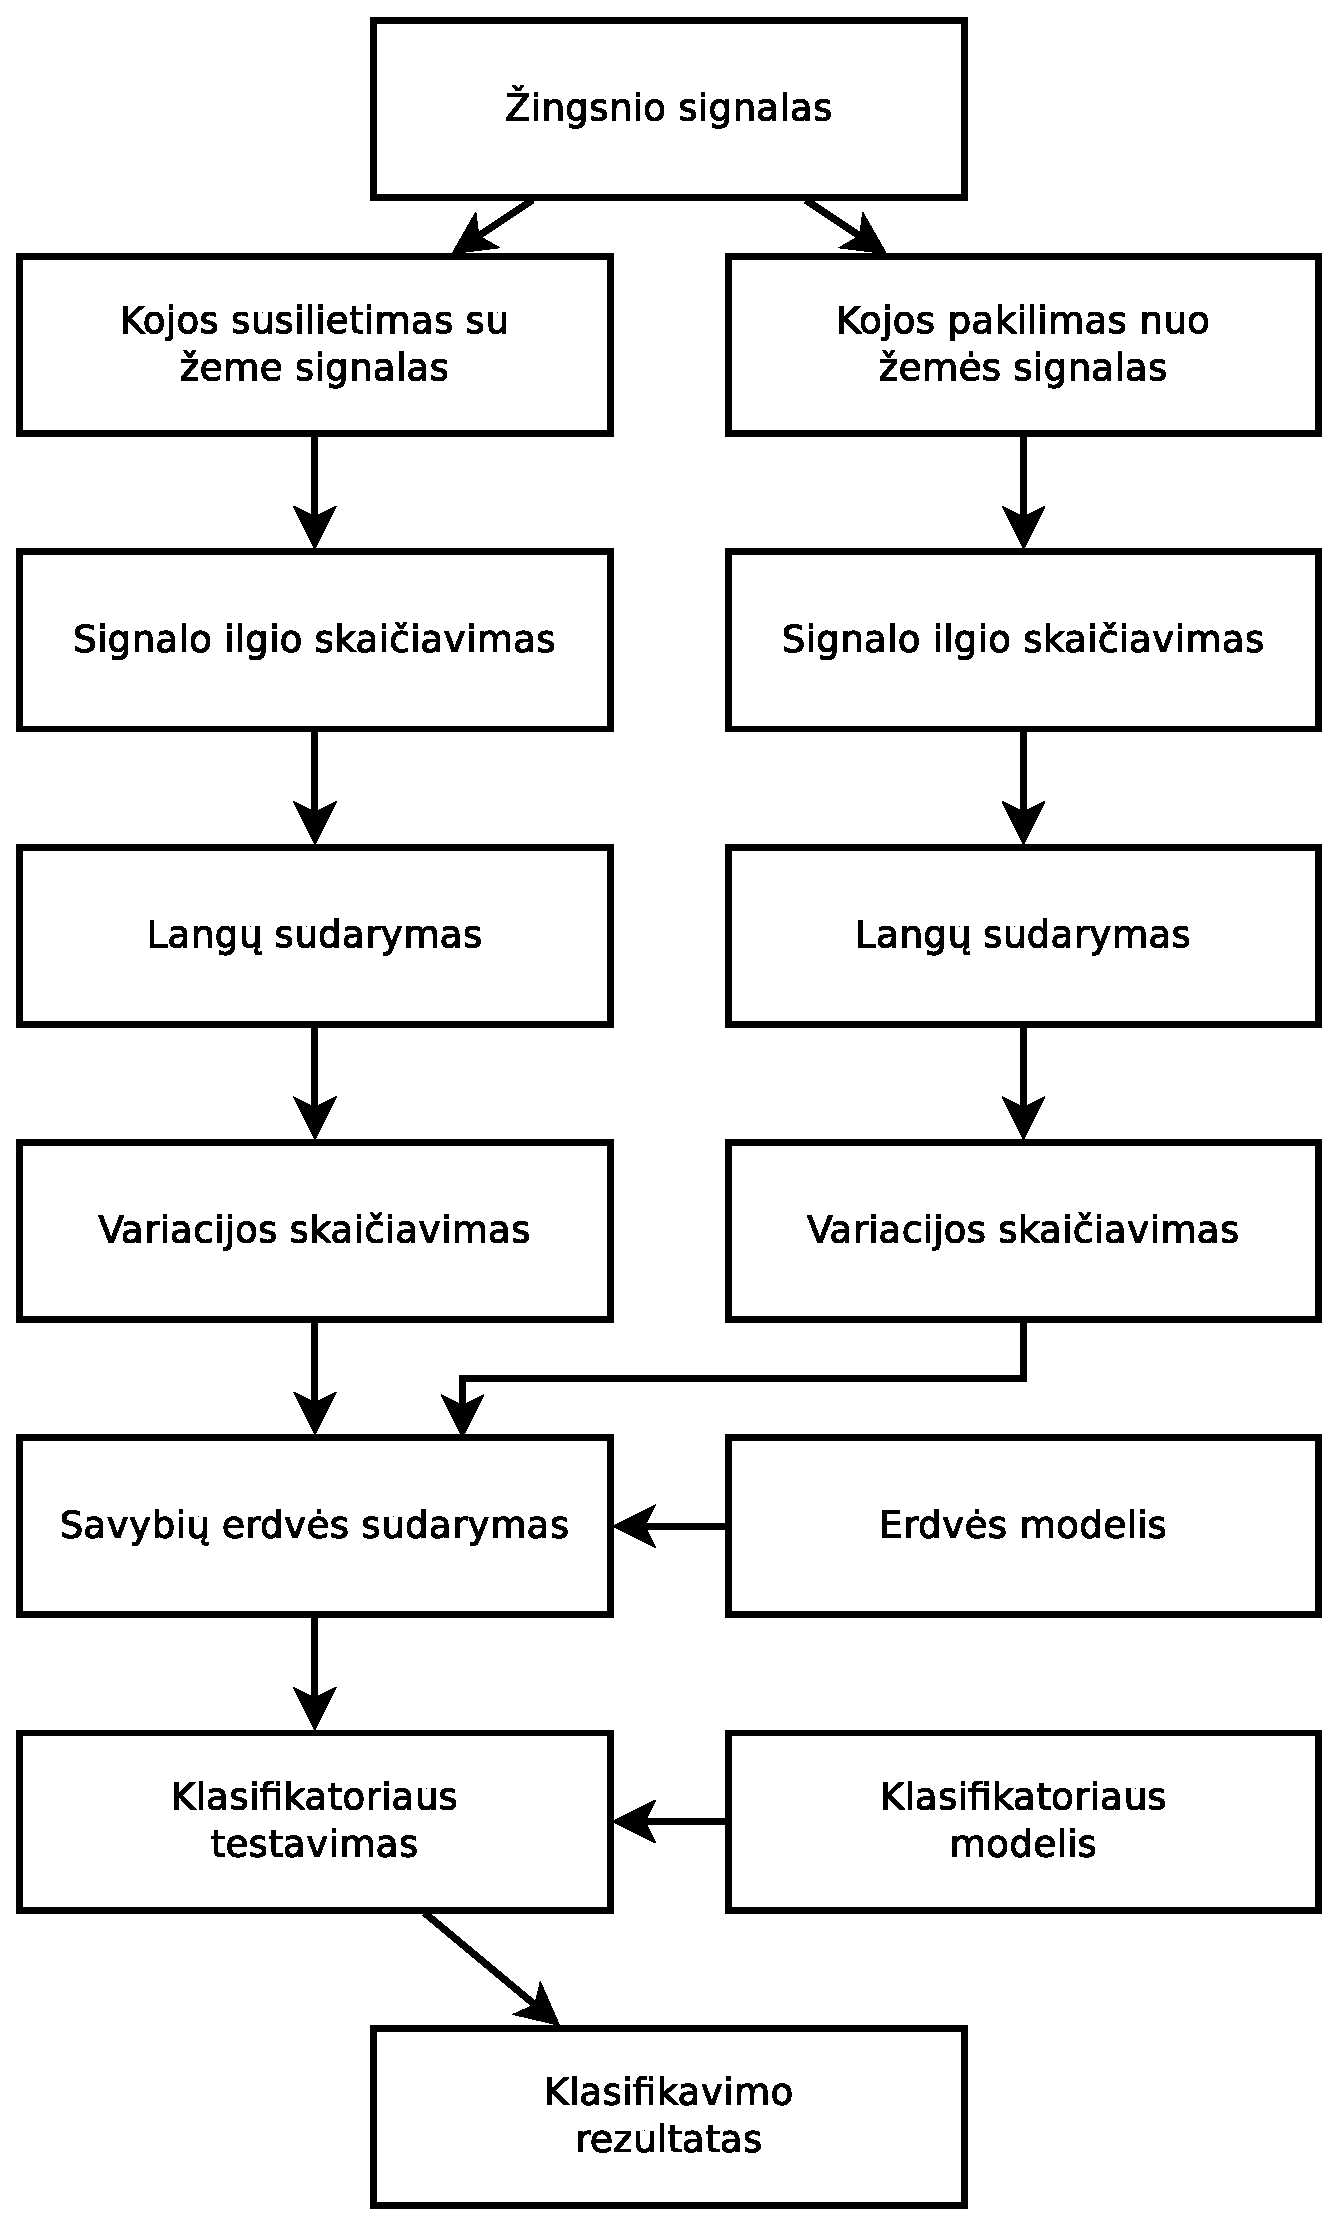
\includegraphics[scale=0.5]{figures/trecia_faze.eps}
  % Graphic for TeX using PGF
% Title: /home/maksim/Documents/Bbd/3_b/figures/trecia_faze.dia
% Creator: Dia v0.97.2
% CreationDate: Thu May 31 00:52:51 2012
% For: maksim
% \usepackage{tikz}
% The following commands are not supported in PSTricks at present
% We define them conditionally, so when they are implemented,
% this pgf file will use them.
\ifx\du\undefined
  \newlength{\du}
\fi
\setlength{\du}{15\unitlength}
\ttfamily\small
\begin{tikzpicture}
\pgftransformxscale{1.000000}
\pgftransformyscale{-1.000000}
\definecolor{dialinecolor}{rgb}{0.000000, 0.000000, 0.000000}
\pgfsetstrokecolor{dialinecolor}
\definecolor{dialinecolor}{rgb}{1.000000, 1.000000, 1.000000}
\pgfsetfillcolor{dialinecolor}
\definecolor{dialinecolor}{rgb}{1.000000, 1.000000, 1.000000}
\pgfsetfillcolor{dialinecolor}
\fill (-1.000000\du,34.000000\du)--(-1.000000\du,37.000000\du)--(9.000000\du,37.000000\du)--(9.000000\du,34.000000\du)--cycle;
\pgfsetlinewidth{0.100000\du}
\pgfsetdash{}{0pt}
\pgfsetdash{}{0pt}
\pgfsetmiterjoin
\definecolor{dialinecolor}{rgb}{0.000000, 0.000000, 0.000000}
\pgfsetstrokecolor{dialinecolor}
\draw (-1.000000\du,34.000000\du)--(-1.000000\du,37.000000\du)--(9.000000\du,37.000000\du)--(9.000000\du,34.000000\du)--cycle;
% setfont left to latex
\definecolor{dialinecolor}{rgb}{0.000000, 0.000000, 0.000000}
\pgfsetstrokecolor{dialinecolor}
\node at (4.000000\du,35.695000\du){Požymių erdvės sudarymas};
\pgfsetlinewidth{0.100000\du}
\pgfsetdash{}{0pt}
\pgfsetdash{}{0pt}
\pgfsetbuttcap
{
\definecolor{dialinecolor}{rgb}{0.000000, 0.000000, 0.000000}
\pgfsetfillcolor{dialinecolor}
% was here!!!
\pgfsetarrowsend{stealth}
\definecolor{dialinecolor}{rgb}{0.000000, 0.000000, 0.000000}
\pgfsetstrokecolor{dialinecolor}
\draw (8.141113\du,32.049072\du)--(5.858887\du,33.950928\du);
}
\definecolor{dialinecolor}{rgb}{1.000000, 1.000000, 1.000000}
\pgfsetfillcolor{dialinecolor}
\fill (11.000000\du,34.000000\du)--(11.000000\du,37.000000\du)--(21.000000\du,37.000000\du)--(21.000000\du,34.000000\du)--cycle;
\pgfsetlinewidth{0.100000\du}
\pgfsetdash{}{0pt}
\pgfsetdash{}{0pt}
\pgfsetmiterjoin
\definecolor{dialinecolor}{rgb}{0.000000, 0.000000, 0.000000}
\pgfsetstrokecolor{dialinecolor}
\draw (11.000000\du,34.000000\du)--(11.000000\du,37.000000\du)--(21.000000\du,37.000000\du)--(21.000000\du,34.000000\du)--cycle;
% setfont left to latex
\definecolor{dialinecolor}{rgb}{0.000000, 0.000000, 0.000000}
\pgfsetstrokecolor{dialinecolor}
\node at (16.000000\du,35.695000\du){Erdvės modelis};
\pgfsetlinewidth{0.100000\du}
\pgfsetdash{}{0pt}
\pgfsetdash{}{0pt}
\pgfsetbuttcap
{
\definecolor{dialinecolor}{rgb}{0.000000, 0.000000, 0.000000}
\pgfsetfillcolor{dialinecolor}
% was here!!!
\pgfsetarrowsend{stealth}
\definecolor{dialinecolor}{rgb}{0.000000, 0.000000, 0.000000}
\pgfsetstrokecolor{dialinecolor}
\draw (10.955078\du,35.500000\du)--(9.044922\du,35.500000\du);
}
\definecolor{dialinecolor}{rgb}{1.000000, 1.000000, 1.000000}
\pgfsetfillcolor{dialinecolor}
\fill (-1.000000\du,39.000000\du)--(-1.000000\du,42.000000\du)--(9.000000\du,42.000000\du)--(9.000000\du,39.000000\du)--cycle;
\pgfsetlinewidth{0.100000\du}
\pgfsetdash{}{0pt}
\pgfsetdash{}{0pt}
\pgfsetmiterjoin
\definecolor{dialinecolor}{rgb}{0.000000, 0.000000, 0.000000}
\pgfsetstrokecolor{dialinecolor}
\draw (-1.000000\du,39.000000\du)--(-1.000000\du,42.000000\du)--(9.000000\du,42.000000\du)--(9.000000\du,39.000000\du)--cycle;
% setfont left to latex
\definecolor{dialinecolor}{rgb}{0.000000, 0.000000, 0.000000}
\pgfsetstrokecolor{dialinecolor}
\node at (4.000000\du,40.295000\du){Klasifikatoriaus};
% setfont left to latex
\definecolor{dialinecolor}{rgb}{0.000000, 0.000000, 0.000000}
\pgfsetstrokecolor{dialinecolor}
\node at (4.000000\du,41.095000\du){testavimas};
\pgfsetlinewidth{0.100000\du}
\pgfsetdash{}{0pt}
\pgfsetdash{}{0pt}
\pgfsetbuttcap
{
\definecolor{dialinecolor}{rgb}{0.000000, 0.000000, 0.000000}
\pgfsetfillcolor{dialinecolor}
% was here!!!
\pgfsetarrowsend{stealth}
\definecolor{dialinecolor}{rgb}{0.000000, 0.000000, 0.000000}
\pgfsetstrokecolor{dialinecolor}
\draw (4.000000\du,37.049072\du)--(4.000000\du,38.950928\du);
}
\definecolor{dialinecolor}{rgb}{1.000000, 1.000000, 1.000000}
\pgfsetfillcolor{dialinecolor}
\fill (11.000000\du,39.000000\du)--(11.000000\du,42.000000\du)--(21.000000\du,42.000000\du)--(21.000000\du,39.000000\du)--cycle;
\pgfsetlinewidth{0.100000\du}
\pgfsetdash{}{0pt}
\pgfsetdash{}{0pt}
\pgfsetmiterjoin
\definecolor{dialinecolor}{rgb}{0.000000, 0.000000, 0.000000}
\pgfsetstrokecolor{dialinecolor}
\draw (11.000000\du,39.000000\du)--(11.000000\du,42.000000\du)--(21.000000\du,42.000000\du)--(21.000000\du,39.000000\du)--cycle;
% setfont left to latex
\definecolor{dialinecolor}{rgb}{0.000000, 0.000000, 0.000000}
\pgfsetstrokecolor{dialinecolor}
\node at (16.000000\du,40.295000\du){Klasifikatoriaus};
% setfont left to latex
\definecolor{dialinecolor}{rgb}{0.000000, 0.000000, 0.000000}
\pgfsetstrokecolor{dialinecolor}
\node at (16.000000\du,41.095000\du){modelis};
\pgfsetlinewidth{0.100000\du}
\pgfsetdash{}{0pt}
\pgfsetdash{}{0pt}
\pgfsetbuttcap
{
\definecolor{dialinecolor}{rgb}{0.000000, 0.000000, 0.000000}
\pgfsetfillcolor{dialinecolor}
% was here!!!
\pgfsetarrowsend{stealth}
\definecolor{dialinecolor}{rgb}{0.000000, 0.000000, 0.000000}
\pgfsetstrokecolor{dialinecolor}
\draw (10.955078\du,40.500000\du)--(9.044922\du,40.500000\du);
}
\definecolor{dialinecolor}{rgb}{1.000000, 1.000000, 1.000000}
\pgfsetfillcolor{dialinecolor}
\fill (5.000000\du,44.000000\du)--(5.000000\du,47.000000\du)--(15.000000\du,47.000000\du)--(15.000000\du,44.000000\du)--cycle;
\pgfsetlinewidth{0.100000\du}
\pgfsetdash{}{0pt}
\pgfsetdash{}{0pt}
\pgfsetmiterjoin
\definecolor{dialinecolor}{rgb}{0.000000, 0.000000, 0.000000}
\pgfsetstrokecolor{dialinecolor}
\draw (5.000000\du,44.000000\du)--(5.000000\du,47.000000\du)--(15.000000\du,47.000000\du)--(15.000000\du,44.000000\du)--cycle;
% setfont left to latex
\definecolor{dialinecolor}{rgb}{0.000000, 0.000000, 0.000000}
\pgfsetstrokecolor{dialinecolor}
\node at (10.000000\du,45.295000\du){Klasifikavimo};
% setfont left to latex
\definecolor{dialinecolor}{rgb}{0.000000, 0.000000, 0.000000}
\pgfsetstrokecolor{dialinecolor}
\node at (10.000000\du,46.095000\du){rezultatas};
\pgfsetlinewidth{0.100000\du}
\pgfsetdash{}{0pt}
\pgfsetdash{}{0pt}
\pgfsetbuttcap
{
\definecolor{dialinecolor}{rgb}{0.000000, 0.000000, 0.000000}
\pgfsetfillcolor{dialinecolor}
% was here!!!
\pgfsetarrowsend{stealth}
\definecolor{dialinecolor}{rgb}{0.000000, 0.000000, 0.000000}
\pgfsetstrokecolor{dialinecolor}
\draw (5.858887\du,42.049072\du)--(8.141113\du,43.950928\du);
}
\definecolor{dialinecolor}{rgb}{1.000000, 1.000000, 1.000000}
\pgfsetfillcolor{dialinecolor}
\fill (5.000000\du,29.000000\du)--(5.000000\du,32.000000\du)--(15.000000\du,32.000000\du)--(15.000000\du,29.000000\du)--cycle;
\pgfsetlinewidth{0.100000\du}
\pgfsetdash{}{0pt}
\pgfsetdash{}{0pt}
\pgfsetmiterjoin
\definecolor{dialinecolor}{rgb}{0.000000, 0.000000, 0.000000}
\pgfsetstrokecolor{dialinecolor}
\draw (5.000000\du,29.000000\du)--(5.000000\du,32.000000\du)--(15.000000\du,32.000000\du)--(15.000000\du,29.000000\du)--cycle;
% setfont left to latex
\definecolor{dialinecolor}{rgb}{0.000000, 0.000000, 0.000000}
\pgfsetstrokecolor{dialinecolor}
\node at (10.000000\du,30.295000\du){Pirminis signalo};
% setfont left to latex
\definecolor{dialinecolor}{rgb}{0.000000, 0.000000, 0.000000}
\pgfsetstrokecolor{dialinecolor}
\node at (10.000000\du,31.095000\du){apdorojimas};
\end{tikzpicture}

  \caption{Trečio modulio, klasifikatoriaus tikrinimo, veikimo schema}
  \label{fig:trecia_faze}
\end{figure}

Apibendrinus bendrą programos veikimo schemą, toliau paanalizuosim patį klasifikavimo mechanizmą -- Naivų Bayes klasifikatorių.

\subsection{Požymių klasifikavimo programos algoritmo schemos sudarymas}
\label{subsec:class_scheme}

Šiame poskyryje apžvelgtas naudojamas klasifikatorius, trumpai aprašytas jo veikimo matematinis principas, įgyvendinimas ir struktūrinė schema.

Naivus Bayes klasifikatorius \cite{R22230} yra paprastas tikimybinis klasifikatorius, kuris paremtas Bayes teorema su stipria duomenų nepriklausomybės prielaida, kuri išreiškiama:

\begin{equation}
	P(\mathbf{X}|C) = \prod_{i=1}^{n} P(X|C),
\end{equation}
kur $\mathbf{X} = (X_1, \cdot \cdot \cdot, X_n)$ yra požymių vektorius, o $C$ yra klasės identifikatorius. Nepriklausomai nuo to, kad tokia duomenų atskyrimo prielaida yra labai naivi -- praktikoje metodas veikia pakankamai gerai, ir yra naudojamas daugelį sudėtingesnių metodikų.

Naivus Bayes klasifikatorius $h^*(x)$, naudoja diskriminanto funkcijas atnaujinti klasės vėlesnes tikimybes, nurodant požymių vektorių:

\begin{equation}
	f^*_i(x) = P(C=i|\mathbf{X}=x).
\end{equation}

Pritaikius Bayes taisyklę nurodytai lygčiai, gaunamas rezultatas:

\begin{equation}
P(C=i|\mathbf{X}=x) = \frac{P(\mathbf{X}=x|C=i)P(C=i)}{P(\mathbf{X}=x)},
\end{equation}
kur $P(\mathbf{X}=x)$ yra identiška visoms klasėms, todėl yra ignoruojama. Iš to seka Bayes diskriminato funkcija:

\begin{equation}
	f^*_i(x) = P(\mathbf{X}=x|C=i)P(C=i),
\end{equation}
kur $P(\mathbf{X}=x|C=i)$ vadinama klasės priklausomybės tikimybės pasiskirstymas. Taigi, Bayes klasifikatorius:

\begin{equation}
h^*(x) = arg max_i P(\mathbf{X}=x|C=i)P(C=i),
\end{equation}
randa didžiausią vėlesnės tikimybės hipotezę, nurodžius $x$.

Duomenys Hilberto erdvėje yra praskiriami tiesinei funkcijai, todėl šiame sprendime yra naudojamas tokios paprastos struktūros klasifikavimo mechanizmas. Tuo labiau, kad duomenys yra vienmatėje erdvėje -- mažinti matmenų skaičių nelieka prasmės, ieškoti klasifikavimo algoritmo, kuris geriausiai apibendrintų turimus duomenis erdvėje nėra prasmės, kadangi duomenų apibendrinimą puikiausiai atliko LDA su Gauso branduoliu.

Darbe panaudota Matlab aplinkoje įgyvendintas naivaus Bayes klasifikatoriaus versija, kuri yra ``Statistical Toolbox'' paketo dalis. Klasifikatoriaus apmokymo kodas yra pateiktas \ref{code:nb_training} programiniam kode. Jo rezultate, kintamajam ''nb`` yra saugomas klasifikatoriaus modelis. Klasifikatoriaus tikrinimo kodas yra pateiktas \ref{code:nb_testing} programiniam kode. Rezultate, kintamajam ``ypred'' yra saugomas programos spėjimas.

\begin{cfigure}
	\centering
	\caption{Klasifikatoriaus apmokymo kodas}
	\label{code:nb_training}
	\begin{lstlisting}
nb = NaiveBayes.fit( training_set.X', training_set.y );
  \end{lstlisting}
\end{cfigure}

\begin{cfigure}
	\centering
	\caption{Klasifikatoriaus tikrinimo kodas}
	\label{code:nb_testing}
	\begin{lstlisting}
ypred = nb.predict( testing_set.X' );
  \end{lstlisting}
\end{cfigure}

Struktūriškai klasifikatoriaus apmokymas yra pateiktas 2 priede \ref{fig:class_train} paveiksle. Programa pradedama nuo signalo variacijos duomenų priėmimo iš pirminio signalo apdorojimo. Pagal ankščiau sukonstruotą erdvės modelį, projektuojami nauji signalo požymiai ir atliekamas klasifikatoriaus apmokymas.

Klasifikatoriaus tikrinimas yra vykdomas pagal 2 priede pateiktą schemą \ref{fig:class_test} paveiksle. Programa pradedama tai pat, kaip ir klasifikatoriaus apmokymas iki ``Erdvės sudarymas pagal požymius'' struktūros bloko. Klasifikatoriaus modelis panaudojamas iš prieš tai atlikto apmokymo ir atliekamas požymių erdvės klasifikavimas. Rezultatai pateikiami neužtikrintumo matrica. Duomenys išvedami vartotojui tikslumo ir atpažinimo skaitiniais įverčiais, ir grafiniu pavidalu.

\subsection{Signalų analizės programos įgyvendinimas}
\label{subsec:total_program}

Šiame poskyryje apžvelgta galutinė programa, aptartos jos pritaikymo problemos, bei galimas pritaikymo platformos.

\begin{figure}
  \centering
%  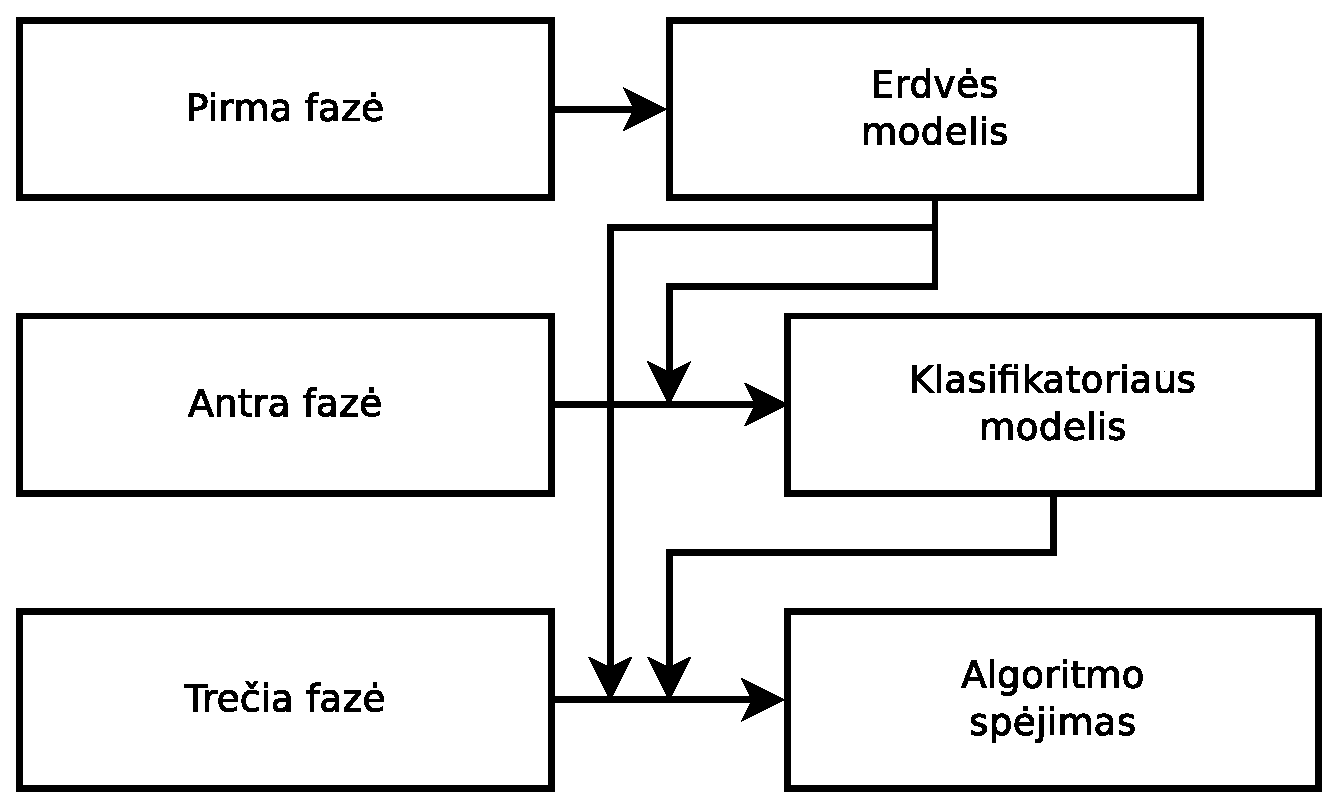
\includegraphics[width=250px]{figures/galutine_programa.eps}
  % Graphic for TeX using PGF
% Title: /home/maksim/Documents/Bbd/3_b/figures/galutine_programa.dia
% Creator: Dia v0.97.2
% CreationDate: Thu May 31 00:45:51 2012
% For: maksim
% \usepackage{tikz}
% The following commands are not supported in PSTricks at present
% We define them conditionally, so when they are implemented,
% this pgf file will use them.
\ifx\du\undefined
  \newlength{\du}
\fi
\setlength{\du}{15\unitlength}
\ttfamily\small
\begin{tikzpicture}
\pgftransformxscale{1.000000}
\pgftransformyscale{-1.000000}
\definecolor{dialinecolor}{rgb}{0.000000, 0.000000, 0.000000}
\pgfsetstrokecolor{dialinecolor}
\definecolor{dialinecolor}{rgb}{1.000000, 1.000000, 1.000000}
\pgfsetfillcolor{dialinecolor}
\definecolor{dialinecolor}{rgb}{1.000000, 1.000000, 1.000000}
\pgfsetfillcolor{dialinecolor}
\fill (5.000000\du,5.000000\du)--(5.000000\du,8.000000\du)--(14.000000\du,8.000000\du)--(14.000000\du,5.000000\du)--cycle;
\pgfsetlinewidth{0.100000\du}
\pgfsetdash{}{0pt}
\pgfsetdash{}{0pt}
\pgfsetmiterjoin
\definecolor{dialinecolor}{rgb}{0.000000, 0.000000, 0.000000}
\pgfsetstrokecolor{dialinecolor}
\draw (5.000000\du,5.000000\du)--(5.000000\du,8.000000\du)--(14.000000\du,8.000000\du)--(14.000000\du,5.000000\du)--cycle;
% setfont left to latex
\definecolor{dialinecolor}{rgb}{0.000000, 0.000000, 0.000000}
\pgfsetstrokecolor{dialinecolor}
\node at (9.500000\du,6.695000\du){Pirmas modulis};
\definecolor{dialinecolor}{rgb}{1.000000, 1.000000, 1.000000}
\pgfsetfillcolor{dialinecolor}
\fill (5.000000\du,10.000000\du)--(5.000000\du,13.000000\du)--(14.000000\du,13.000000\du)--(14.000000\du,10.000000\du)--cycle;
\pgfsetlinewidth{0.100000\du}
\pgfsetdash{}{0pt}
\pgfsetdash{}{0pt}
\pgfsetmiterjoin
\definecolor{dialinecolor}{rgb}{0.000000, 0.000000, 0.000000}
\pgfsetstrokecolor{dialinecolor}
\draw (5.000000\du,10.000000\du)--(5.000000\du,13.000000\du)--(14.000000\du,13.000000\du)--(14.000000\du,10.000000\du)--cycle;
% setfont left to latex
\definecolor{dialinecolor}{rgb}{0.000000, 0.000000, 0.000000}
\pgfsetstrokecolor{dialinecolor}
\node at (9.500000\du,11.695000\du){Antras modulis};
\definecolor{dialinecolor}{rgb}{1.000000, 1.000000, 1.000000}
\pgfsetfillcolor{dialinecolor}
\fill (5.000000\du,15.000000\du)--(5.000000\du,18.000000\du)--(14.000000\du,18.000000\du)--(14.000000\du,15.000000\du)--cycle;
\pgfsetlinewidth{0.100000\du}
\pgfsetdash{}{0pt}
\pgfsetdash{}{0pt}
\pgfsetmiterjoin
\definecolor{dialinecolor}{rgb}{0.000000, 0.000000, 0.000000}
\pgfsetstrokecolor{dialinecolor}
\draw (5.000000\du,15.000000\du)--(5.000000\du,18.000000\du)--(14.000000\du,18.000000\du)--(14.000000\du,15.000000\du)--cycle;
% setfont left to latex
\definecolor{dialinecolor}{rgb}{0.000000, 0.000000, 0.000000}
\pgfsetstrokecolor{dialinecolor}
\node at (9.500000\du,16.695000\du){Trečias modulis};
\definecolor{dialinecolor}{rgb}{1.000000, 1.000000, 1.000000}
\pgfsetfillcolor{dialinecolor}
\fill (16.000000\du,5.000000\du)--(16.000000\du,8.000000\du)--(25.000000\du,8.000000\du)--(25.000000\du,5.000000\du)--cycle;
\pgfsetlinewidth{0.100000\du}
\pgfsetdash{}{0pt}
\pgfsetdash{}{0pt}
\pgfsetmiterjoin
\definecolor{dialinecolor}{rgb}{0.000000, 0.000000, 0.000000}
\pgfsetstrokecolor{dialinecolor}
\draw (16.000000\du,5.000000\du)--(16.000000\du,8.000000\du)--(25.000000\du,8.000000\du)--(25.000000\du,5.000000\du)--cycle;
% setfont left to latex
\definecolor{dialinecolor}{rgb}{0.000000, 0.000000, 0.000000}
\pgfsetstrokecolor{dialinecolor}
\node at (20.500000\du,6.295000\du){Erdvės};
% setfont left to latex
\definecolor{dialinecolor}{rgb}{0.000000, 0.000000, 0.000000}
\pgfsetstrokecolor{dialinecolor}
\node at (20.500000\du,7.095000\du){modelis};
\definecolor{dialinecolor}{rgb}{1.000000, 1.000000, 1.000000}
\pgfsetfillcolor{dialinecolor}
\fill (18.000000\du,10.000000\du)--(18.000000\du,13.000000\du)--(27.000000\du,13.000000\du)--(27.000000\du,10.000000\du)--cycle;
\pgfsetlinewidth{0.100000\du}
\pgfsetdash{}{0pt}
\pgfsetdash{}{0pt}
\pgfsetmiterjoin
\definecolor{dialinecolor}{rgb}{0.000000, 0.000000, 0.000000}
\pgfsetstrokecolor{dialinecolor}
\draw (18.000000\du,10.000000\du)--(18.000000\du,13.000000\du)--(27.000000\du,13.000000\du)--(27.000000\du,10.000000\du)--cycle;
% setfont left to latex
\definecolor{dialinecolor}{rgb}{0.000000, 0.000000, 0.000000}
\pgfsetstrokecolor{dialinecolor}
\node at (22.500000\du,11.295000\du){Klasifikatoriaus};
% setfont left to latex
\definecolor{dialinecolor}{rgb}{0.000000, 0.000000, 0.000000}
\pgfsetstrokecolor{dialinecolor}
\node at (22.500000\du,12.095000\du){modelis};
\definecolor{dialinecolor}{rgb}{1.000000, 1.000000, 1.000000}
\pgfsetfillcolor{dialinecolor}
\fill (18.000000\du,15.000000\du)--(18.000000\du,18.000000\du)--(27.000000\du,18.000000\du)--(27.000000\du,15.000000\du)--cycle;
\pgfsetlinewidth{0.100000\du}
\pgfsetdash{}{0pt}
\pgfsetdash{}{0pt}
\pgfsetmiterjoin
\definecolor{dialinecolor}{rgb}{0.000000, 0.000000, 0.000000}
\pgfsetstrokecolor{dialinecolor}
\draw (18.000000\du,15.000000\du)--(18.000000\du,18.000000\du)--(27.000000\du,18.000000\du)--(27.000000\du,15.000000\du)--cycle;
% setfont left to latex
\definecolor{dialinecolor}{rgb}{0.000000, 0.000000, 0.000000}
\pgfsetstrokecolor{dialinecolor}
\node at (22.500000\du,16.295000\du){Algoritmo};
% setfont left to latex
\definecolor{dialinecolor}{rgb}{0.000000, 0.000000, 0.000000}
\pgfsetstrokecolor{dialinecolor}
\node at (22.500000\du,17.095000\du){spėjimas};
\pgfsetlinewidth{0.100000\du}
\pgfsetdash{}{0pt}
\pgfsetdash{}{0pt}
\pgfsetbuttcap
{
\definecolor{dialinecolor}{rgb}{0.000000, 0.000000, 0.000000}
\pgfsetfillcolor{dialinecolor}
% was here!!!
\pgfsetarrowsend{stealth}
\definecolor{dialinecolor}{rgb}{0.000000, 0.000000, 0.000000}
\pgfsetstrokecolor{dialinecolor}
\draw (14.049988\du,6.500000\du)--(15.950012\du,6.500000\du);
}
\pgfsetlinewidth{0.100000\du}
\pgfsetdash{}{0pt}
\pgfsetdash{}{0pt}
\pgfsetbuttcap
{
\definecolor{dialinecolor}{rgb}{0.000000, 0.000000, 0.000000}
\pgfsetfillcolor{dialinecolor}
% was here!!!
\pgfsetarrowsend{stealth}
\definecolor{dialinecolor}{rgb}{0.000000, 0.000000, 0.000000}
\pgfsetstrokecolor{dialinecolor}
\draw (14.000000\du,11.500000\du)--(18.000000\du,11.500000\du);
}
\pgfsetlinewidth{0.100000\du}
\pgfsetdash{}{0pt}
\pgfsetdash{}{0pt}
\pgfsetbuttcap
{
\definecolor{dialinecolor}{rgb}{0.000000, 0.000000, 0.000000}
\pgfsetfillcolor{dialinecolor}
% was here!!!
\pgfsetarrowsend{stealth}
\definecolor{dialinecolor}{rgb}{0.000000, 0.000000, 0.000000}
\pgfsetstrokecolor{dialinecolor}
\draw (14.050079\du,16.500000\du)--(17.949921\du,16.500000\du);
}
\pgfsetlinewidth{0.100000\du}
\pgfsetdash{}{0pt}
\pgfsetdash{}{0pt}
\pgfsetmiterjoin
\pgfsetbuttcap
{
\definecolor{dialinecolor}{rgb}{0.000000, 0.000000, 0.000000}
\pgfsetfillcolor{dialinecolor}
% was here!!!
\pgfsetarrowsend{stealth}
{\pgfsetcornersarced{\pgfpoint{0.000000\du}{0.000000\du}}\definecolor{dialinecolor}{rgb}{0.000000, 0.000000, 0.000000}
\pgfsetstrokecolor{dialinecolor}
\draw (20.500000\du,8.050171\du)--(20.500000\du,9.500000\du)--(16.000000\du,9.500000\du)--(16.000000\du,11.500000\du);
}}
\pgfsetlinewidth{0.100000\du}
\pgfsetdash{}{0pt}
\pgfsetdash{}{0pt}
\pgfsetmiterjoin
\pgfsetbuttcap
{
\definecolor{dialinecolor}{rgb}{0.000000, 0.000000, 0.000000}
\pgfsetfillcolor{dialinecolor}
% was here!!!
\pgfsetarrowsend{stealth}
{\pgfsetcornersarced{\pgfpoint{0.000000\du}{0.000000\du}}\definecolor{dialinecolor}{rgb}{0.000000, 0.000000, 0.000000}
\pgfsetstrokecolor{dialinecolor}
\draw (22.500000\du,13.049072\du)--(22.500000\du,14.000000\du)--(16.000000\du,14.000000\du)--(16.000000\du,16.500000\du);
}}
\pgfsetlinewidth{0.100000\du}
\pgfsetdash{}{0pt}
\pgfsetdash{}{0pt}
\pgfsetmiterjoin
\pgfsetbuttcap
{
\definecolor{dialinecolor}{rgb}{0.000000, 0.000000, 0.000000}
\pgfsetfillcolor{dialinecolor}
% was here!!!
\pgfsetarrowsend{stealth}
{\pgfsetcornersarced{\pgfpoint{0.000000\du}{0.000000\du}}\definecolor{dialinecolor}{rgb}{0.000000, 0.000000, 0.000000}
\pgfsetstrokecolor{dialinecolor}
\draw (20.500000\du,8.048828\du)--(20.500000\du,8.500000\du)--(15.000000\du,8.500000\du)--(15.000000\du,16.500000\du)--(15.000000\du,16.500000\du);
}}
\end{tikzpicture}

  \caption{Galutinės programos struktūrinė schema}
  \label{fig:galutine_programa}
\end{figure}

Galutinė programos schema atvaizduota \ref{fig:galutine_programa} paveiksle. Kaip aptarta ankstesniuose poskyriuose -- programa susideda iš trijų duomenų apdorojimo modulių. Kiekvieno modulio veikimas pradedamas nuo pirminio signalo apdorojimo duomenų, tačiau kiekvieno modulio rezultatas yra skirtingas. Kiekvienas žemiau esantis modulis naudoja virš jos esančio modulio darbo rezultatą. Kritiškai svarbu yra kiekvienam moduliui pateikti skirtingus duomenis.

Darbe pateiktas metodas leidžia efektyviai atpažinti ar subjektas serga Parkinsono liga. Didžiausias metodo trūkumas yra neatsižvelgimas į kitus Parkinsono ligos simptomus -- drebulys, eisenos sustingimas. Drebulys gali pasireikšti ne tik plaštakos raumenyse, tačiau ir kaklo srityje. Tai neleidžia tiksliai apibrėžti kurią kūno vietą reikia stebėti ir rinkti duomenis tyrimui. Eisenos sustingimas taip pat yra sunkiai apibrėžtas faktorius, kadangi jo aptikimas yra labai didelis iššūkis signalų apdorojimo srityje. Geriausią ką šiuo metu gali pasiūlyti mokslas, stebint tokius ligos simptomus -- paciento stebėjimas vaizdo kameros pagalba, jo veiklos automatinis nustatymas. Drebulys subjektui dažniausiai pasireiškia, kai jo kūnas yra visiškai atsipalaidavęs, t.y. kai subjektas stovi, sėdi, guli, kai jis išlaiko statišką poziciją. Kameros pagalba galima nustatyti kokioje pozicijoje yra subjektas, tačiau identifikuoti drebulį yra labai sudėtinga, jeigu naudojama kamera yra mažos raiškos. Drebulį veiklos nustatymo algoritmas gali palaikyti tiesiog pašaliniu triukšmu, kaip šešėlio sudarymą ant stebimo paviršiaus. 

Parkinsono ligos identifikavimo ir jo diagnozavimo reikalauja papildomų tyrimų. Besivystant kompiuteriniai technikai, bei atsirandant vis naujiems algoritmams nestandartinėms problemoms spręsti -- šansas, kad ateityje šios ligos diagnozavimas pagerės, išlieka labai didelis.

\section{Signalų analizės programos patikra}

Šiame skyriuje parengtas ir įgyvendintas algoritmo patikros planas. Programos patikra yra kritinis aspektas jos patikimumo tikrinimui. Algoritmą galima tikrinti mažinant apmokymo verčių skaičių ir didinant tikrinimo verčių kiekį -- taip sužinant kiek mažiausiai verčių reikia metodui, norint pilnai apibendrinti turimus duomenis.

Tikrinant kiekvieno žmogaus žingsnio signalus, paaiškėjo, kad skirtingi subjektai sugeneruoja kitokį tikrinimui tinkamų žingsnių skaičių, todėl tikrinimas atliekamas ne atskiriant konkrečius žmones, o jau išskirtus kojos pakilimo ir kojos prisilietimo prie žemės signalus, konkrečiau -- iš tų signalų suformuotus jų ilgių duomenų langus.

Po pirminio duomenų apdorojimo, kontrolinių subjektų grupėje liko $1790$ duomenų langų, Parkinsono subjektų grupėje liko $1619$ duomenų langų, todėl nuspręsta iš kiekvienos grupės pasiimti po $1500$ langų duomenų, visi jie padalinti po lygias tris dalis: viena dalis erdvės sudarymui, antra dalis klasifikatoriaus apmokymui, trečia dalis klasifikatoriaus testavimui. Jokie duomenys jokioje dalyje pasikartotinai nesikartoja. Tai yra kritinis faktorius mašininiam apmokyme \cite{824819}. Taip pat reikia užtikrinti duomenų praskyrimo ir klasifikatoriaus apmokymui dešimtį kartų didesnių duomenų skaičių, negu yra tų pačių duomenų matmenų. Kadangi prieš duomenų klasifikavimą turimi tik $d=2$ matmenys, tai teoriškai užtektų ir $n=21$ ($n/d > 10$). Užtikrinant erdvės apibendrinimą, matmenų praskyrimas vyksta su $500$ taškų rinkiniu. 

\subsection{Eksperimentų plano rengimas}

Šiame poskyryje aptarti galimi eksperimentiniai algoritmo patikros planai, nurodytas galimos duomenų pateikimo metodikos.

Pirminį patikros planą sudaro pateikiamų duomenų skaičiaus mažinimas į kiekvieno algoritmo žingsnį: matmenų erdvės sudarymas, klasifikatoriaus apmokymas, klasifikatoriaus testavimas. Duomenis galima mažinti tiesiniu būdu -- matmenų mažinime naudoti pirmus $400$ duomenų, $100$ praleisti, nuo $501$ iki $1000$ paduodi klasifikatoriaus apmokymui ir nuo $1001$ iki $1500$ pateikti klasifikatoriaus tikrinimui. Taip pat duomenis galima pateikti kas kelintą $n$ narį -- kadangi iš viso yra trys algoritmo žingsniai, tuomet $n=3$. Taip į matmenų mažinimo algoritmą pateikiamas pirmas rinkinys, ketvirtas rinkinys, septintas rinkinys. Klasifikatoriaus apmokymui pateikiamas antras rinkinys, penktas rinkinys, aštuntas rinkinys. Klasifikatoriaus tikrinimui pateikiamas trečias rinkinys, šeštas rinkinys, devintas rinkinys. Nurodytas duomenų pateikimas yra naudojamas, siekiant kiekvienam programos moduliui pateikti skirtingesnius duomenis. 

Kadangi sprendime naudojamas laikinos atminties modulis, kuris reikalingas saugoti pirmąjį diskriminantą kiekvienos variacijos poros, eksperimentiniu būdu galima spręsti koks lango dydis nurodytai užduočiai atlikti geriausiai tinka. Atliekant tokį tikrinimą svarbu išlaikyti kitų parametrų skaičiaus vienodumą, todėl į kiekvieną iš trijų modulių pateikiamas pastovus duomenų skaičius, kuomet keičiamas laikinos atminties dydis. Tikrinimas taip pat nuspręs kiek minimaliai iš paciento eisenos turi būti išskirta požymių grupių, kad sistema grąžintų geriausią klasifikavimo tikslumo ir atpažinimo rezultatą.

\subsection{Duomenų eksperimentams rengimas}

Šiame poskyryje aptartas duomenų eksperimentams rengimas, aprašytas planuojamas duomenų kiekis, naudojamas tikrinimo metu.

Pradžioje yra tikrinamas matmenų mažinimo algoritmas, mažinant pateikiamų duomenų skaičių. Struktūriškai nuspręsta, kad kiekvienas modulis turi lygiai po $500$ rinkinių. Tikrinimas pradedamas nuo $500$ rinkinių ir mažinamas kas $100$ rinkinių. Vadinasi, iš viso matmenų mažinimo algoritmui pateikiama $500$, $400$, $300$, $200$, $100$ ir minimalus $21$ rinkinių skaičius. Į apmokymo lygmenį pateikiamas pastovus duomenų skaičius -- $500$ (nuo $501$ iki $1000$) rinkinių. Laikinos atminties dydis palaikomas pastovus -- $50$ verčių. Po matmenų mažinimo žingsnio tikrinimo, rinkinių skaičius tokia pat metodika mažinamas klasifikatoriaus apmokymui, matmenų mažinimo metodui pateikiant pastovų rinkinių skaičių. Šioje stadijoje duomenų skaičius nėra mažinamas iki $21$ rinkinio skaičiaus, kadangi neformuojamas naudojamas lango ilgio, $50$, duomenų skaičius. Klasifikatoriaus testavimo atveju duomenų dydis nėra mažinamas.

Laikinos atminties ilgio tikrinimo metu panaudoti tokie laikinos atminties ilgiai: $10$, $30$, $50$, $70$, $100$, $130$ ir $150$. Kiekvienas toks tikinimas atliekamas su duomenų kiekiu, kuris parodė geriausią klasifikavimo tikslumo ir atpažinimo rezultatą, aprašytą ankstesniame paragrafe. Panaudoti rezultatai atitinkamai užtikrins optimalų duomenų kiekio pasiskirstymą, geriausiam klasifikavimo tikslumo ir atpažinimo rezultatui pasiekti.

% Kokie duomenys ir kodėl bus naudojami patikrai?

\subsection{Programos patikros rezultatai}
\begin{table}
	\centering
	\renewcommand{\arraystretch}{1.3}
	\caption{Klasifikavimo rezultatai, tiesiškai mažinant pateikiamų duomenų matmenų mažinimo algoritmui}
	\label{table:first_phase_experiment}
	\begin{tabular}{|c|c|c|c|c|c|c|c|} \hline
			& & \multicolumn{6}{c|}{Taškų rinkinio skaičius} \\ \cline{3-8}
						&	& 500 	& 400	& 300 	& 200 & 100 	& 21 	\\ \hline
		\multirow{2}{*}{Co}
		& Tikslumas	& $0,700$ & $\mathbf{0,800}$ & $0,450$ & $0,450$ & $0,500$ & $0,450$ \\ \cline{2-8}
		& Atpažinimas  &	$0,750$ & $\mathbf{0,875}$ & $0,467$ & $0,429$ & $0,500$ & $0,400$ \\ \hline
		\multirow{2}{*}{Pt}
		& Tikslumas	& $0,700$ & $\mathbf{0,800}$ & $0,450$ & $0,450$ & $0,500$ & $0,450$ \\ \cline{2-8}
		& Atpažinimas  &	$0,667$ & $\mathbf{0,750}$ & $0,400$ & $0,462$ & $0,500$ & $0,467$ \\ \hline
	\end{tabular}
\end{table}

\begin{table}
	\centering
	\renewcommand{\arraystretch}{1.3}
	\caption{Klasifikavimo rezultatai, tiesiškai mažinant pateikiamų duomenų klasifikatoriaus apmokymo algoritmui}
	\label{table:second_phase_experiment}
	\begin{tabular}{|c|c|c|c|c|c|c|c|} \hline
			& & \multicolumn{6}{c|}{Taškų rinkinio skaičius} \\ \cline{3-8}
						&	& 500 	& 400	& 300 	& 200 & 100 	& 21 	\\ \hline
		\multirow{2}{*}{Co}
		& Tikslumas	& $\mathbf{0,800}$ & $\mathbf{0,800}$ & $0,750$ & $0,750$ & $0,650$ & $-$ \\ \cline{2-8}
		& Atpažinimas  &	$\mathbf{0,875}$ & $\mathbf{0,875}$ & $0,857$ & $1,000$ & $1,000$ & $-$ \\ \hline
		\multirow{2}{*}{Pt}
		& Tikslumas	& $\mathbf{0,800}$ & $\mathbf{0,800}$ & $0,750$ & $0,750$ & $0,650$ & $-$ \\ \cline{2-8}
		& Atpažinimas  &	$\mathbf{0,750}$ & $\mathbf{0,750}$ & $0,692$ & $0,667$ & $0,588$ & $-$ \\ \hline
	\end{tabular}
\end{table}

Šiame poskyryje pateikti ir aptarti patikros tikslumo ir atpažinimo rezultatai, išanalizuoti galimi sistemos parametrai, kurie gali būti derinami: duomenų skaičius, kuris naudojamas kiekvienam programos moduliui, bei atminties dydis, kuris naudojamas pirmajai diskriminanto vertei saugoti.

Pirma patikra atlikta tiesiškai mažinant duomenų kiekį, kuris yra paduodamas matmenų mažinimo algoritmui, taip siekiant nustatyti koks duomenų kiekis geriausiai tinka naujai požymių erdvei projektuoti. Eksperimentiniai duomenys yra pateikti \ref{table:first_phase_experiment} lentelėje. Vertinant matmenų sudarymą pagal klasifikatoriaus duodamą rezultatą, geriausias duomenų kiekis, skirtas naujai matmenų erdvei sudaryti yra $400$ erdvės taškų. Tokiu atveju pasiekiamas $0,875$ Pt ir $0,750$ Co atpažinimas. 

Antra patikra atlikta tiesiškai mažinant duomenų kiekį, kuris yra paduodamas klasifikatoriaus apmokymui, taip siekiant nustatyti, kokio duomenų kiekio reikia klasifikatoriui, kad jis sugebėtų apibendrinti duomenis, naudojamus testavimo stadijoje. Eksperimentiniai duomenys yra pateikti \ref{table:second_phase_experiment} lentelėje. Šio tikrinimo metu paaiškėjo, kad geriausiai klasifikatoriaus apmokymui tinka du duomenų rinkiniai -- po $500$ ir po $400$. Tokiu atveju pasirenkamas didesnis duomenų kiekis, taip užtikrinant bendrų duomenų apibrėžtumą.

\begin{table}
	\centering
	\renewcommand{\arraystretch}{1.3}
	\caption{Klasifikavimo rezultatai, netiesiškai mažinant pateikiamų duomenų matmenų mažinimo algoritmui}
	\label{table:first_phase_not_linear_experiment}
	\begin{tabular}{|c|c|c|c|c|c|c|c|} \hline
			& & \multicolumn{6}{c|}{Taškų rinkinio skaičius} \\ \cline{3-8}
						&	& 500 	& 400	& 300 	& 200 & 100 	& 21 	\\ \hline
		\multirow{2}{*}{Co}
		& Tikslumas & $0,550$ & $0,450$ & $0,600$ & $0,600$ & $0,450$ & $\mathbf{0,650}$ \\ \cline{2-8}
		& Atpažinimas & $0,533$ & $0,467$ & $0,583$ & $0,583$ & $0,400$ & $\mathbf{0,667}$ \\ \hline
		\multirow{2}{*}{Pt}
		& Tikslumas & $0,550$ & $0,450$ & $0,600$ & $0,600$ & $0,450$ & $\mathbf{0,650}$ \\ \cline{2-8}
		& Atpažinimas & $0,600$ & $0,400$ & $0,625$ & $0,625$ & $0,467$ & $\mathbf{0,636}$ \\ \hline
	\end{tabular}
\end{table}

\begin{table}
	\centering
	\renewcommand{\arraystretch}{1.3}
	\caption{Klasifikavimo rezultatai, netiesiškai mažinant pateikiamų duomenų klasifikatoriaus apmokymo algoritmui}
	\label{table:second_phase_not_linear_experiment}
	\begin{tabular}{|c|c|c|c|c|c|c|c|} \hline
			& & \multicolumn{6}{c|}{Taškų rinkinio skaičius} \\ \cline{3-8}
						&	& 500 	& 400	& 300 	& 200 & 100 	& 21 	\\ \hline
		\multirow{2}{*}{Co}
		& Tikslumas	& $0,550$ & $0,450$ & $0,500$ & $0,400$ & $\mathbf{0,550}$ & $-$ \\ \cline{2-8}
		& Atpažinimas  &	$0,553$ & $0,455$ & $0,500$ & $0,400$ & $\mathbf{1,000}$ & $-$ \\ \hline
		\multirow{2}{*}{Pt}
		& Tikslumas	& $0,550$ & $0,450$ & $0,500$ & $0,400$ & $\mathbf{0,550}$ & $-$ \\ \cline{2-8}
		& Atpažinimas  &	$0,600$ & $0,444$ & $0,500$ & $0,400$ & $\mathbf{0,526}$ & $-$ \\ \hline
	\end{tabular}
\end{table}

\begin{table}
	\centering
	\renewcommand{\arraystretch}{1.3}
	\caption{Klasifikavimo rezultatai, mažinant laikinosios atminties dydį}
	\label{table:memory_linear_experiment}
	\begin{tabular}{|c|c|c|c|c|c|c|c|c|} \hline
			& & \multicolumn{7}{c|}{Laikinosios atminties dydis} \\ \cline{3-9}
						&	& 150 & 130 & 100 & 70 & 50 & 30 & 10\\ \hline
		\multirow{2}{*}{Co}
									%150				%130			%100				%70				%50			% 30				%10
		& Tikslumas	& $0,500$ & $0,500$ & $0,700$ & $0,500$ & $\mathbf{0,800}$ & $0,500$ & $0,570$ \\ \cline{2-9}
		& Atpažinimas &	$0,500$ & $0,500$ & $0,750$ & $0,500$ & $\mathbf{0,875}$ & $0,500$ & $0,585$ \\ \hline
		\multirow{2}{*}{Pt}
		& Tikslumas	& $0,500$ & $0,500$ & $0,700$ & $0,500$ & $\mathbf{0,800}$ & $0,500$ & $0,570$ \\ \cline{2-9}
		& Atpažinimas &	$0,500$ & $0,500$ & $0,667$ & $0,500$ & $\mathbf{0,750}$ & $0,500$ & $0,559$ \\ \hline
	\end{tabular}
\end{table}

Trečia patikra atlikta netiesiškai mažinant duomenų kiekį, kuris yra paduodamas matmenų mažinimo algoritmui. Klasifikavimo rezultatai yra pateikiami \ref{table:first_phase_not_linear_experiment} lentelėje. Bendri klasifikavimo tikslumo ir atpažinimo rezultatai yra prastesni, negu mažinant duomenų pateikimą tiesiniu būdu, todėl iš eksperimento galima teigti, kad duomenis į matmenų mažinimo algoritmą geriausiai yra pateikti tiesiniu būdu -- nuo $1$ eilės iki $400$ eilės numerio. Taip duomenis yra geriau ``apibendrinami'' matmenų mažinimo algoritmo, ką parodo klasifikavimo rezultatas.

Ketvirta patikra atlikta netiesiškai mažinant duomenų kiekį, kuris yra paduodamas klasifikatoriaus apmokymo metodui. Klasifikavimo rezultatai yra pateikiami \ref{table:second_phase_not_linear_experiment} lentelėje. Kaip ir trečios patikros atveju -- klasifikavimo duomenis nėra patenkinami, todėl ir klasifikavimo apmokymo atveju, duomenis geriausiai pateikti tiesiniu būdu -- nuo $0$  eilės iki $500$ eilės numerio.

Paskutinė patikra atlikta keičiant laikinosios atminties dydžio matmenis. Duomenų erdvei sudaryti panaudoti duomenys, gauti pirmos patikros metu, klasifikatoriaus apmokymui panaudoti duomenys, gauti antros patikros metu. Klasifikavimo rezultatai yra pateikti \ref{table:memory_linear_experiment} lentelėje. Geriausias laikinosios atminties lango dydis, prie kurio pasiekiamas geriausias klasifikavimo rezultatas yra $50$ pirmojo diskriminanto verčių.

Iš pateiktos analizės, priimti tokie sistemos veikimo parametrai:
\begin{itemize}
\item Naujai duomenų erdvei konstruoti panaudoti duomenis nuo $1$ iki $400$ eilės numerio;
\item Klasifikatoriaus apmokymui panaudoti duomenis nuo $500$ iki $1000$ eilės numerio;
\item Laikinosios atminties dydis, kuriame saugomos pirmojo disktriminato vertės, $50$ eilės.
\end{itemize}

Patikros metu nustatyta, kad programa geriausiai veikia $80~\%$ tikslumu, kas įveda nepasitikėjimo faktorių, kuris lygus $1/5$ visų rezultatų tikslumu. Toks rezultatas yra geras tik tuo atveju, jeigu aprašytas diagnostikos įrankis panaudotas mažiausiai penkis kartus, norint pateikti galutinę diagnozę, kad pacientas turi arba neturi Parkinsono ligos, pagal eisenos sutrikimo simptomus.

\section{Rezultatų apibendrinimas}

% Ar buvo pasiektas užsibrėžtas tikslas?

Darbo metu ištirti galimi žingsnio požymiai, kuriais remiantis galima sėkmingai atpažinti Parkinsono ligą pagal subjekto eiseną. Nustatyta, kad dažninės žingsnio komponentės, koreliacijos koeficientas, dviejų maksimumų ir vieno minimumo požymiai neturi pakankamai informacijos Parkinsono ligos atpažinimui. Daugiausiai informacijos turi kojos prisilietimo prie žemės ir kojos pakilimo nuo žemės signalo laiko variacijos požymis.

Turint duomenis, kurie turi daugiausiai informacijos ligos identifikavimui, toliau patikrinta galimų matmenų praskyrimo metodų pritaikymas. Tiesiniai PCA ir LDA transformacijos metodai požymių erdvės tinkamai nepraskyrė. Geriausiai užduotį LDA transformacija su Gauso branduoliu. Pritaikius nagrinėjamas transformacijas duomenų grupėms, pastebėta kaip branduolio metodo pritaikymas gali padidinti matmenų mažinimo algoritmo efektyvumą.

% Kiek gerai veikia sukurtas produktas?

Turimus vienmačius duomenis realiu laiku geriausiai klasifikavo Naivus Bayes klasifikatorius, tačiau klasifikavimo tikslumas ir atpažinimas yra nepatenkinamas, tikslumas siekė tik $50,8~\%$. Pritaikius papildomą metodikos žingsnį -- laikinosios atminties bloką, kuriame saugomas pirmas transformacijos diskriminantas, klasifikavimo tikslumas pagerintas iki $80~\%$. Rezultatas nurodo kas penkto diagnozavimo rezultato klaidingumą. Turint omenyje, kad klinikinės diagnostikos sprendimų atpažinimas yra nuo $74~\%$ iki $90~\%$ \cite{vgtu}, sistemos darbo rezultatas kitų produktų palyginime atrodo patenkinamai.

% Ar visus iškeltus uždavinius pavyko sėkmingai išspręsti, įgyvendinti?

Pagrindinis darbo uždavinys buvo sukurti sistemą, kuri gebėtų atpažinti Parkinsono ligą pagal galimus ligos požymius, nagrinėjant subjektus pagal jų eisenos ypatybes. Toks uždavinys yra įvykdytas, tačiau egzistuoja $1/5$ dalies netikslumas. Toks netikslumas argumentuojamas kiekvieno žmogaus eisenos unikaliomis savybėmis. Tokia neigiama metodo savybė yra pašalinama, atliekant diagnozę mažiausiai $5$ kartus.

Darbe planuotas naudoti dirbtinių neuronų tinklas panaudotas nebuvo. Duomenys požymių erdvėje buvo lengvai atskiriami tiesine funkcija, todėl naudoti kompleksinio dirbtinių neuronų tinklų klasifikatorių nėra prasmės. Panaudotas paprastesnis naivaus Bayes klasifikatorius.

Naudojamų subjektų skaičius klasifikatoriaus apmokymui ir tikrinimui panaudotas nebuvo. Iš viso, klasifikatoriaus apmokymui planuota panaudoti $60$ Parkinsono liga sergančių ir $50$ kontrolinių subjektų. Klasifikatoriaus tikrinimui planuota panaudoti $33$ sergančių ir $23$ sveikų subjektų. Kiekvienas iš subjektų generuoja skirtingą skaičių patikrintų žingsnių signalų, iš kurių toliau skaičiuojami požymiai. Duomenų analizės metu, norint suvienodinti ir tuo pačiu supaprastinti uždavinio nagrinėjimą, pirmiausiai iš kiekvieno subjekto išskirti žingsnio fazės signalai ir jie visi sujungti į vieną matricą. Tuomet egzistuoja dvi matricos, kurios priklauso skirtingai subjektų grupei. Toliau dalinti duomenis pagal kiekvieno subjektu sugeneruotų duomenų kiekį nėra prasmės, kadangi pirmiausiai yra naudojamas skirtingas subjektų skaičius kiekvienos grupės atžvilgiu ir yra garantuojamas duomenų skaičiaus neatitikimas. Skaičiaus atitikimas yra būtinas erdvės transformacijai atlikti, todėl reikia suvienodinti esamų duomenų skaičių. Tikrinimo atveju turi būti atliekama tokia pati procedūrą. Dėl šios priežasties buvo parinktas visų esamų duomenų dalinimas į tris lygias dalis kiekvieno programos modulio įgyvendinimui.

% Ką reiktų, galima būtų daryti kitaip, norint pagerinti gautus rezultatus ?

Gautus rezultatus galima pagerinti, išnagrinėjus daugiau kontrolinių subjektų eisenos ypatybių, bei Parkinsono liga sergančių subjektų eisenos ypatybes. Iš viso buvo išnagrinėti $93$ sergantys subjektai ir $73$ sveikas subjektas. Iš sveikų subjektų iš viso buvo išskirta $3543$ kojos pakilimo nuo žemės signalų, $3583$ kojos prisilietimo prie žemės signalai. Iš sergančių subjektų iš viso buvo išskirta $3241$ kojos pakilimo nuo žemės signalų, $3217$ kojos prisilietimo prie žemės signalai. Iš gautų signalų buvo paskaičiuota jų ilgiai ir naudojantis slankiojančio lango metodu -- jų variacija. Iš viso, sveikų subjektų buvo požymių buvo $1790$, sergančių subjektų požymių $1619$ verčių. Nurodyto darbo rezultatus gali patikslinti tik dar didesnis subjektų skaičius, bei ilgesnis eisenos laikas, kuris šių duomenų atveju buvo tik $2~min$.

% Ar pasirinktos darbo priemonės pateisino lūkeščius?

Darbe panaudotos priemonės lūkesčius pateisino iš dalies. Išskirtas požymis identifikuoja ligos požymius tik esant ilgos eisenos prielaidai -- subjektas turi atlikti eisenos patikrą ilgiau negu $2~min$. Rekomenduojama eisenos trukmė yra $5~min$. Tokiu atveju sistema geriausiai identifikuos ligos simptomą pagal parinktus požymius. Taip pat klasifikavimo rezultatus gali pagerinti abiejų kojų naudojimas požymių išskyrimo metu, kadangi eisenos nesimetriškumas gali galioti ne tik kairiai kūno pusei, tačiau ir dešinei.

\addcontentsline{toc}{section}{Literatūros ir informacinių šaltinių sąrašas}
\renewcommand\refname{Literatūros ir informacinių šaltinių sąrašas}

\bibliographystyle{plain}
\bibliography{references}

\section*{Santrauka}
\addcontentsline{toc}{section}{Santrauka}

The goal of the Bachelor thesis was to develop an application, which is capable of Parkinson's disease recognition from gait analysis. The work was started from the alternatives methods review, with discussion of drawbacks and advantages. Based on this review, the methods, which will be used in this work, was derived. The second step was to find the features of the signals, which would most effectively separate the Parkinson's subjects from control subjects. The most logical feature had problems in feature space, so the dimensional reduction method had to be applied. The classification mechanism was chosen very simple, because of the one-dimensional data in feature space and classification only of two classes with no further information. System verification confirmed, that system is able to recognize Parkinson's subjects, but additional experiments with more data must be made.

\section*{PRIEDAI}
\addcontentsline{toc}{section}{PRIEDAI}

\subsection*{1 priedas. PCA įgyvendinimas, panaudojus skirtingas metodikas.}
\label{subsec:pca_source}

\begin{cfigure}[!h]
  \centering
  \caption{PCA įgyvendinimas, panaudojus SVD}
  \label{code:pca_svd}
  \lstinputlisting{sources/pca2.m}
\end{cfigure}

\begin{cfigure}[H]
  \centering
  \caption{PCA įgyvendinimas, panaudojus tikrinių vektorių dekompoziciją}
  \label{code:pca_eig}
  \lstinputlisting{sources/pca1.m}
\end{cfigure}

\subsection*{2 priedas. Požymio klasifikavimo programos algoritmo schemos}
\label{subsec:class_stuff}

\begin{figure}[H]
  \centering
%  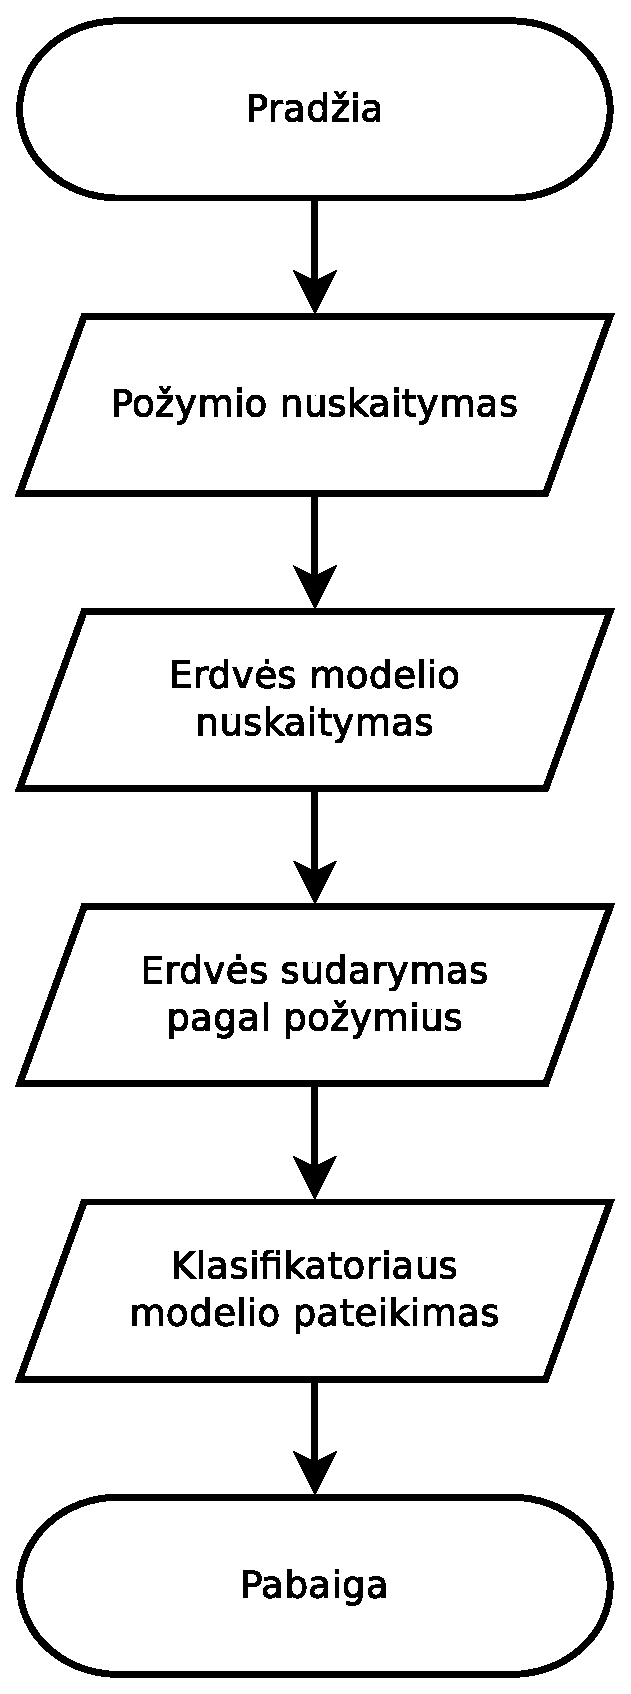
\includegraphics[scale=0.5]{figures/klasifikatoriaus_apmokymas.eps}
  % Graphic for TeX using PGF
% Title: /home/maksim/Documents/Bbd/3_b/figures/klasifikatoriaus_apmokymas.dia
% Creator: Dia v0.97.2
% CreationDate: Thu May 31 00:47:27 2012
% For: maksim
% \usepackage{tikz}
% The following commands are not supported in PSTricks at present
% We define them conditionally, so when they are implemented,
% this pgf file will use them.
\ifx\du\undefined
  \newlength{\du}
\fi
\setlength{\du}{15\unitlength}
\ttfamily\small
\begin{tikzpicture}
\pgftransformxscale{1.000000}
\pgftransformyscale{-1.000000}
\definecolor{dialinecolor}{rgb}{0.000000, 0.000000, 0.000000}
\pgfsetstrokecolor{dialinecolor}
\definecolor{dialinecolor}{rgb}{1.000000, 1.000000, 1.000000}
\pgfsetfillcolor{dialinecolor}
\definecolor{dialinecolor}{rgb}{1.000000, 1.000000, 1.000000}
\pgfsetfillcolor{dialinecolor}
\fill (21.091911\du,9.000000\du)--(30.000000\du,9.000000\du)--(28.908089\du,12.000000\du)--(20.000000\du,12.000000\du)--cycle;
\pgfsetlinewidth{0.100000\du}
\pgfsetdash{}{0pt}
\pgfsetdash{}{0pt}
\pgfsetmiterjoin
\definecolor{dialinecolor}{rgb}{0.000000, 0.000000, 0.000000}
\pgfsetstrokecolor{dialinecolor}
\draw (21.091911\du,9.000000\du)--(30.000000\du,9.000000\du)--(28.908089\du,12.000000\du)--(20.000000\du,12.000000\du)--cycle;
% setfont left to latex
\definecolor{dialinecolor}{rgb}{0.000000, 0.000000, 0.000000}
\pgfsetstrokecolor{dialinecolor}
\node at (25.000000\du,10.695000\du){Požymio nuskaitymas};
\pgfsetlinewidth{0.100000\du}
\pgfsetdash{}{0pt}
\pgfsetdash{}{0pt}
\pgfsetbuttcap
\pgfsetmiterjoin
\pgfsetlinewidth{0.100000\du}
\pgfsetbuttcap
\pgfsetmiterjoin
\pgfsetdash{}{0pt}
\definecolor{dialinecolor}{rgb}{1.000000, 1.000000, 1.000000}
\pgfsetfillcolor{dialinecolor}
\pgfpathmoveto{\pgfpoint{21.666667\du}{4.000000\du}}
\pgfpathlineto{\pgfpoint{28.333333\du}{4.000000\du}}
\pgfpathcurveto{\pgfpoint{29.253808\du}{4.000000\du}}{\pgfpoint{30.000000\du}{4.671572\du}}{\pgfpoint{30.000000\du}{5.500000\du}}
\pgfpathcurveto{\pgfpoint{30.000000\du}{6.328428\du}}{\pgfpoint{29.253808\du}{7.000000\du}}{\pgfpoint{28.333333\du}{7.000000\du}}
\pgfpathlineto{\pgfpoint{21.666667\du}{7.000000\du}}
\pgfpathcurveto{\pgfpoint{20.746192\du}{7.000000\du}}{\pgfpoint{20.000000\du}{6.328428\du}}{\pgfpoint{20.000000\du}{5.500000\du}}
\pgfpathcurveto{\pgfpoint{20.000000\du}{4.671572\du}}{\pgfpoint{20.746192\du}{4.000000\du}}{\pgfpoint{21.666667\du}{4.000000\du}}
\pgfusepath{fill}
\definecolor{dialinecolor}{rgb}{0.000000, 0.000000, 0.000000}
\pgfsetstrokecolor{dialinecolor}
\pgfpathmoveto{\pgfpoint{21.666667\du}{4.000000\du}}
\pgfpathlineto{\pgfpoint{28.333333\du}{4.000000\du}}
\pgfpathcurveto{\pgfpoint{29.253808\du}{4.000000\du}}{\pgfpoint{30.000000\du}{4.671572\du}}{\pgfpoint{30.000000\du}{5.500000\du}}
\pgfpathcurveto{\pgfpoint{30.000000\du}{6.328428\du}}{\pgfpoint{29.253808\du}{7.000000\du}}{\pgfpoint{28.333333\du}{7.000000\du}}
\pgfpathlineto{\pgfpoint{21.666667\du}{7.000000\du}}
\pgfpathcurveto{\pgfpoint{20.746192\du}{7.000000\du}}{\pgfpoint{20.000000\du}{6.328428\du}}{\pgfpoint{20.000000\du}{5.500000\du}}
\pgfpathcurveto{\pgfpoint{20.000000\du}{4.671572\du}}{\pgfpoint{20.746192\du}{4.000000\du}}{\pgfpoint{21.666667\du}{4.000000\du}}
\pgfusepath{stroke}
% setfont left to latex
\definecolor{dialinecolor}{rgb}{0.000000, 0.000000, 0.000000}
\pgfsetstrokecolor{dialinecolor}
\node at (25.000000\du,5.700000\du){Pradžia};
\definecolor{dialinecolor}{rgb}{1.000000, 1.000000, 1.000000}
\pgfsetfillcolor{dialinecolor}
\fill (21.091911\du,14.000000\du)--(30.000000\du,14.000000\du)--(28.908089\du,17.000000\du)--(20.000000\du,17.000000\du)--cycle;
\pgfsetlinewidth{0.100000\du}
\pgfsetdash{}{0pt}
\pgfsetdash{}{0pt}
\pgfsetmiterjoin
\definecolor{dialinecolor}{rgb}{0.000000, 0.000000, 0.000000}
\pgfsetstrokecolor{dialinecolor}
\draw (21.091911\du,14.000000\du)--(30.000000\du,14.000000\du)--(28.908089\du,17.000000\du)--(20.000000\du,17.000000\du)--cycle;
% setfont left to latex
\definecolor{dialinecolor}{rgb}{0.000000, 0.000000, 0.000000}
\pgfsetstrokecolor{dialinecolor}
\node at (25.000000\du,15.295000\du){Erdvės modelio};
% setfont left to latex
\definecolor{dialinecolor}{rgb}{0.000000, 0.000000, 0.000000}
\pgfsetstrokecolor{dialinecolor}
\node at (25.000000\du,16.095000\du){nuskaitymas};
\definecolor{dialinecolor}{rgb}{1.000000, 1.000000, 1.000000}
\pgfsetfillcolor{dialinecolor}
\fill (21.091911\du,19.000000\du)--(30.000000\du,19.000000\du)--(28.908089\du,22.000000\du)--(20.000000\du,22.000000\du)--cycle;
\pgfsetlinewidth{0.100000\du}
\pgfsetdash{}{0pt}
\pgfsetdash{}{0pt}
\pgfsetmiterjoin
\definecolor{dialinecolor}{rgb}{0.000000, 0.000000, 0.000000}
\pgfsetstrokecolor{dialinecolor}
\draw (21.091911\du,19.000000\du)--(30.000000\du,19.000000\du)--(28.908089\du,22.000000\du)--(20.000000\du,22.000000\du)--cycle;
% setfont left to latex
\definecolor{dialinecolor}{rgb}{0.000000, 0.000000, 0.000000}
\pgfsetstrokecolor{dialinecolor}
\node at (25.000000\du,20.295000\du){Erdvės sudarymas};
% setfont left to latex
\definecolor{dialinecolor}{rgb}{0.000000, 0.000000, 0.000000}
\pgfsetstrokecolor{dialinecolor}
\node at (25.000000\du,21.095000\du){pagal požymius};
\definecolor{dialinecolor}{rgb}{1.000000, 1.000000, 1.000000}
\pgfsetfillcolor{dialinecolor}
\fill (21.091911\du,24.000000\du)--(30.000000\du,24.000000\du)--(28.908089\du,27.000000\du)--(20.000000\du,27.000000\du)--cycle;
\pgfsetlinewidth{0.100000\du}
\pgfsetdash{}{0pt}
\pgfsetdash{}{0pt}
\pgfsetmiterjoin
\definecolor{dialinecolor}{rgb}{0.000000, 0.000000, 0.000000}
\pgfsetstrokecolor{dialinecolor}
\draw (21.091911\du,24.000000\du)--(30.000000\du,24.000000\du)--(28.908089\du,27.000000\du)--(20.000000\du,27.000000\du)--cycle;
% setfont left to latex
\definecolor{dialinecolor}{rgb}{0.000000, 0.000000, 0.000000}
\pgfsetstrokecolor{dialinecolor}
\node at (25.000000\du,25.295000\du){Klasifikatoriaus};
% setfont left to latex
\definecolor{dialinecolor}{rgb}{0.000000, 0.000000, 0.000000}
\pgfsetstrokecolor{dialinecolor}
\node at (25.000000\du,26.095000\du){modelio pateikimas};
\pgfsetlinewidth{0.100000\du}
\pgfsetdash{}{0pt}
\pgfsetdash{}{0pt}
\pgfsetbuttcap
\pgfsetmiterjoin
\pgfsetlinewidth{0.100000\du}
\pgfsetbuttcap
\pgfsetmiterjoin
\pgfsetdash{}{0pt}
\definecolor{dialinecolor}{rgb}{1.000000, 1.000000, 1.000000}
\pgfsetfillcolor{dialinecolor}
\pgfpathmoveto{\pgfpoint{21.666667\du}{29.000000\du}}
\pgfpathlineto{\pgfpoint{28.333333\du}{29.000000\du}}
\pgfpathcurveto{\pgfpoint{29.253808\du}{29.000000\du}}{\pgfpoint{30.000000\du}{29.671572\du}}{\pgfpoint{30.000000\du}{30.500000\du}}
\pgfpathcurveto{\pgfpoint{30.000000\du}{31.328428\du}}{\pgfpoint{29.253808\du}{32.000000\du}}{\pgfpoint{28.333333\du}{32.000000\du}}
\pgfpathlineto{\pgfpoint{21.666667\du}{32.000000\du}}
\pgfpathcurveto{\pgfpoint{20.746192\du}{32.000000\du}}{\pgfpoint{20.000000\du}{31.328428\du}}{\pgfpoint{20.000000\du}{30.500000\du}}
\pgfpathcurveto{\pgfpoint{20.000000\du}{29.671572\du}}{\pgfpoint{20.746192\du}{29.000000\du}}{\pgfpoint{21.666667\du}{29.000000\du}}
\pgfusepath{fill}
\definecolor{dialinecolor}{rgb}{0.000000, 0.000000, 0.000000}
\pgfsetstrokecolor{dialinecolor}
\pgfpathmoveto{\pgfpoint{21.666667\du}{29.000000\du}}
\pgfpathlineto{\pgfpoint{28.333333\du}{29.000000\du}}
\pgfpathcurveto{\pgfpoint{29.253808\du}{29.000000\du}}{\pgfpoint{30.000000\du}{29.671572\du}}{\pgfpoint{30.000000\du}{30.500000\du}}
\pgfpathcurveto{\pgfpoint{30.000000\du}{31.328428\du}}{\pgfpoint{29.253808\du}{32.000000\du}}{\pgfpoint{28.333333\du}{32.000000\du}}
\pgfpathlineto{\pgfpoint{21.666667\du}{32.000000\du}}
\pgfpathcurveto{\pgfpoint{20.746192\du}{32.000000\du}}{\pgfpoint{20.000000\du}{31.328428\du}}{\pgfpoint{20.000000\du}{30.500000\du}}
\pgfpathcurveto{\pgfpoint{20.000000\du}{29.671572\du}}{\pgfpoint{20.746192\du}{29.000000\du}}{\pgfpoint{21.666667\du}{29.000000\du}}
\pgfusepath{stroke}
% setfont left to latex
\definecolor{dialinecolor}{rgb}{0.000000, 0.000000, 0.000000}
\pgfsetstrokecolor{dialinecolor}
\node at (25.000000\du,30.700000\du){Pabaiga};
\pgfsetlinewidth{0.100000\du}
\pgfsetdash{}{0pt}
\pgfsetdash{}{0pt}
\pgfsetbuttcap
{
\definecolor{dialinecolor}{rgb}{0.000000, 0.000000, 0.000000}
\pgfsetfillcolor{dialinecolor}
% was here!!!
\pgfsetarrowsend{stealth}
\definecolor{dialinecolor}{rgb}{0.000000, 0.000000, 0.000000}
\pgfsetstrokecolor{dialinecolor}
\draw (25.000000\du,7.049072\du)--(25.000000\du,8.950928\du);
}
\pgfsetlinewidth{0.100000\du}
\pgfsetdash{}{0pt}
\pgfsetdash{}{0pt}
\pgfsetbuttcap
{
\definecolor{dialinecolor}{rgb}{0.000000, 0.000000, 0.000000}
\pgfsetfillcolor{dialinecolor}
% was here!!!
\pgfsetarrowsend{stealth}
\definecolor{dialinecolor}{rgb}{0.000000, 0.000000, 0.000000}
\pgfsetstrokecolor{dialinecolor}
\draw (25.000000\du,12.049072\du)--(25.000000\du,13.950928\du);
}
\pgfsetlinewidth{0.100000\du}
\pgfsetdash{}{0pt}
\pgfsetdash{}{0pt}
\pgfsetbuttcap
{
\definecolor{dialinecolor}{rgb}{0.000000, 0.000000, 0.000000}
\pgfsetfillcolor{dialinecolor}
% was here!!!
\pgfsetarrowsend{stealth}
\definecolor{dialinecolor}{rgb}{0.000000, 0.000000, 0.000000}
\pgfsetstrokecolor{dialinecolor}
\draw (25.000000\du,17.049072\du)--(25.000000\du,18.950928\du);
}
\pgfsetlinewidth{0.100000\du}
\pgfsetdash{}{0pt}
\pgfsetdash{}{0pt}
\pgfsetbuttcap
{
\definecolor{dialinecolor}{rgb}{0.000000, 0.000000, 0.000000}
\pgfsetfillcolor{dialinecolor}
% was here!!!
\pgfsetarrowsend{stealth}
\definecolor{dialinecolor}{rgb}{0.000000, 0.000000, 0.000000}
\pgfsetstrokecolor{dialinecolor}
\draw (25.000000\du,22.049072\du)--(25.000000\du,23.950928\du);
}
\pgfsetlinewidth{0.100000\du}
\pgfsetdash{}{0pt}
\pgfsetdash{}{0pt}
\pgfsetbuttcap
{
\definecolor{dialinecolor}{rgb}{0.000000, 0.000000, 0.000000}
\pgfsetfillcolor{dialinecolor}
% was here!!!
\pgfsetarrowsend{stealth}
\definecolor{dialinecolor}{rgb}{0.000000, 0.000000, 0.000000}
\pgfsetstrokecolor{dialinecolor}
\draw (25.000000\du,27.049072\du)--(25.000000\du,28.950928\du);
}
\end{tikzpicture}

  \caption{Klasifikatoriaus apmokymo schema}
  \label{fig:class_train}
\end{figure}

\begin{figure}[H]
  \centering
%  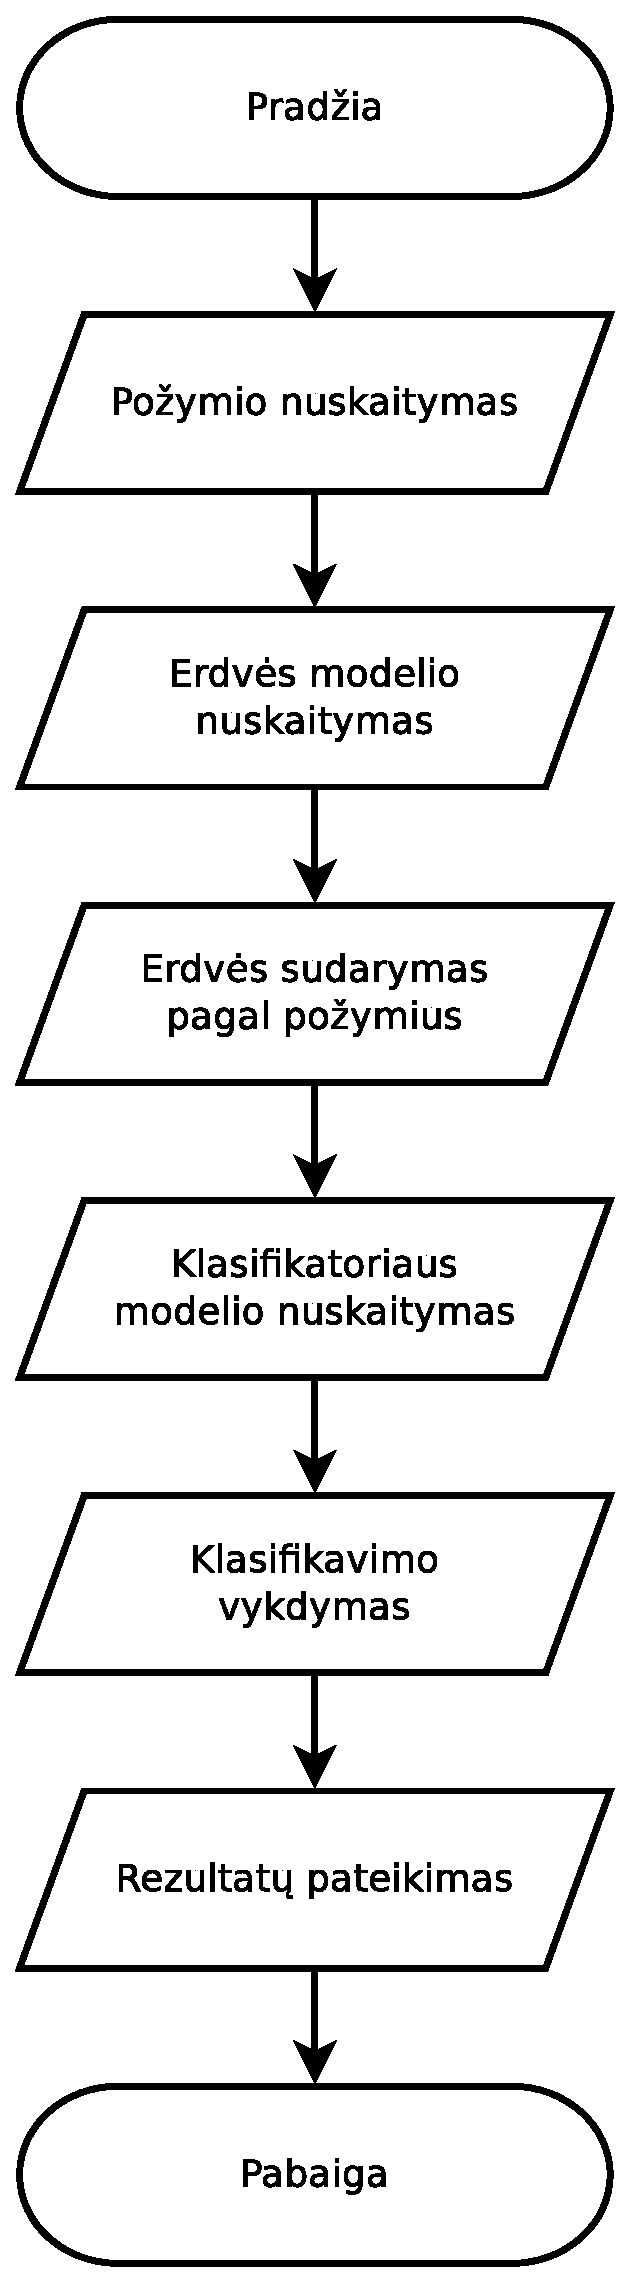
\includegraphics[scale=0.5]{figures/klasifkatoriaus_tikrinimas.eps}
  % Graphic for TeX using PGF
% Title: /home/maksim/Documents/Bbd/3_b/figures/klasifikatoriaus_tikrinimas.dia
% Creator: Dia v0.97.2
% CreationDate: Thu May 31 00:49:55 2012
% For: maksim
% \usepackage{tikz}
% The following commands are not supported in PSTricks at present
% We define them conditionally, so when they are implemented,
% this pgf file will use them.
\ifx\du\undefined
  \newlength{\du}
\fi
\setlength{\du}{15\unitlength}
\ttfamily\small
\begin{tikzpicture}
\pgftransformxscale{1.000000}
\pgftransformyscale{-1.000000}
\definecolor{dialinecolor}{rgb}{0.000000, 0.000000, 0.000000}
\pgfsetstrokecolor{dialinecolor}
\definecolor{dialinecolor}{rgb}{1.000000, 1.000000, 1.000000}
\pgfsetfillcolor{dialinecolor}
\definecolor{dialinecolor}{rgb}{1.000000, 1.000000, 1.000000}
\pgfsetfillcolor{dialinecolor}
\fill (8.091911\du,8.000000\du)--(17.000000\du,8.000000\du)--(15.908089\du,11.000000\du)--(7.000000\du,11.000000\du)--cycle;
\pgfsetlinewidth{0.100000\du}
\pgfsetdash{}{0pt}
\pgfsetdash{}{0pt}
\pgfsetmiterjoin
\definecolor{dialinecolor}{rgb}{0.000000, 0.000000, 0.000000}
\pgfsetstrokecolor{dialinecolor}
\draw (8.091911\du,8.000000\du)--(17.000000\du,8.000000\du)--(15.908089\du,11.000000\du)--(7.000000\du,11.000000\du)--cycle;
% setfont left to latex
\definecolor{dialinecolor}{rgb}{0.000000, 0.000000, 0.000000}
\pgfsetstrokecolor{dialinecolor}
\node at (12.000000\du,9.695000\du){Požymio nuskaitymas};
\pgfsetlinewidth{0.100000\du}
\pgfsetdash{}{0pt}
\pgfsetdash{}{0pt}
\pgfsetbuttcap
\pgfsetmiterjoin
\pgfsetlinewidth{0.100000\du}
\pgfsetbuttcap
\pgfsetmiterjoin
\pgfsetdash{}{0pt}
\definecolor{dialinecolor}{rgb}{1.000000, 1.000000, 1.000000}
\pgfsetfillcolor{dialinecolor}
\pgfpathmoveto{\pgfpoint{8.666667\du}{3.000000\du}}
\pgfpathlineto{\pgfpoint{15.333333\du}{3.000000\du}}
\pgfpathcurveto{\pgfpoint{16.253808\du}{3.000000\du}}{\pgfpoint{17.000000\du}{3.671572\du}}{\pgfpoint{17.000000\du}{4.500000\du}}
\pgfpathcurveto{\pgfpoint{17.000000\du}{5.328428\du}}{\pgfpoint{16.253808\du}{6.000000\du}}{\pgfpoint{15.333333\du}{6.000000\du}}
\pgfpathlineto{\pgfpoint{8.666667\du}{6.000000\du}}
\pgfpathcurveto{\pgfpoint{7.746192\du}{6.000000\du}}{\pgfpoint{7.000000\du}{5.328428\du}}{\pgfpoint{7.000000\du}{4.500000\du}}
\pgfpathcurveto{\pgfpoint{7.000000\du}{3.671572\du}}{\pgfpoint{7.746192\du}{3.000000\du}}{\pgfpoint{8.666667\du}{3.000000\du}}
\pgfusepath{fill}
\definecolor{dialinecolor}{rgb}{0.000000, 0.000000, 0.000000}
\pgfsetstrokecolor{dialinecolor}
\pgfpathmoveto{\pgfpoint{8.666667\du}{3.000000\du}}
\pgfpathlineto{\pgfpoint{15.333333\du}{3.000000\du}}
\pgfpathcurveto{\pgfpoint{16.253808\du}{3.000000\du}}{\pgfpoint{17.000000\du}{3.671572\du}}{\pgfpoint{17.000000\du}{4.500000\du}}
\pgfpathcurveto{\pgfpoint{17.000000\du}{5.328428\du}}{\pgfpoint{16.253808\du}{6.000000\du}}{\pgfpoint{15.333333\du}{6.000000\du}}
\pgfpathlineto{\pgfpoint{8.666667\du}{6.000000\du}}
\pgfpathcurveto{\pgfpoint{7.746192\du}{6.000000\du}}{\pgfpoint{7.000000\du}{5.328428\du}}{\pgfpoint{7.000000\du}{4.500000\du}}
\pgfpathcurveto{\pgfpoint{7.000000\du}{3.671572\du}}{\pgfpoint{7.746192\du}{3.000000\du}}{\pgfpoint{8.666667\du}{3.000000\du}}
\pgfusepath{stroke}
% setfont left to latex
\definecolor{dialinecolor}{rgb}{0.000000, 0.000000, 0.000000}
\pgfsetstrokecolor{dialinecolor}
\node at (12.000000\du,4.700000\du){Pradžia};
\definecolor{dialinecolor}{rgb}{1.000000, 1.000000, 1.000000}
\pgfsetfillcolor{dialinecolor}
\fill (8.091911\du,13.000000\du)--(17.000000\du,13.000000\du)--(15.908089\du,16.000000\du)--(7.000000\du,16.000000\du)--cycle;
\pgfsetlinewidth{0.100000\du}
\pgfsetdash{}{0pt}
\pgfsetdash{}{0pt}
\pgfsetmiterjoin
\definecolor{dialinecolor}{rgb}{0.000000, 0.000000, 0.000000}
\pgfsetstrokecolor{dialinecolor}
\draw (8.091911\du,13.000000\du)--(17.000000\du,13.000000\du)--(15.908089\du,16.000000\du)--(7.000000\du,16.000000\du)--cycle;
% setfont left to latex
\definecolor{dialinecolor}{rgb}{0.000000, 0.000000, 0.000000}
\pgfsetstrokecolor{dialinecolor}
\node at (12.000000\du,14.295000\du){Erdvės modelio};
% setfont left to latex
\definecolor{dialinecolor}{rgb}{0.000000, 0.000000, 0.000000}
\pgfsetstrokecolor{dialinecolor}
\node at (12.000000\du,15.095000\du){nuskaitymas};
\definecolor{dialinecolor}{rgb}{1.000000, 1.000000, 1.000000}
\pgfsetfillcolor{dialinecolor}
\fill (8.091911\du,18.000000\du)--(17.000000\du,18.000000\du)--(15.908089\du,21.000000\du)--(7.000000\du,21.000000\du)--cycle;
\pgfsetlinewidth{0.100000\du}
\pgfsetdash{}{0pt}
\pgfsetdash{}{0pt}
\pgfsetmiterjoin
\definecolor{dialinecolor}{rgb}{0.000000, 0.000000, 0.000000}
\pgfsetstrokecolor{dialinecolor}
\draw (8.091911\du,18.000000\du)--(17.000000\du,18.000000\du)--(15.908089\du,21.000000\du)--(7.000000\du,21.000000\du)--cycle;
% setfont left to latex
\definecolor{dialinecolor}{rgb}{0.000000, 0.000000, 0.000000}
\pgfsetstrokecolor{dialinecolor}
\node at (12.000000\du,19.295000\du){Erdvės sudarymas};
% setfont left to latex
\definecolor{dialinecolor}{rgb}{0.000000, 0.000000, 0.000000}
\pgfsetstrokecolor{dialinecolor}
\node at (12.000000\du,20.095000\du){pagal požymius};
\definecolor{dialinecolor}{rgb}{1.000000, 1.000000, 1.000000}
\pgfsetfillcolor{dialinecolor}
\fill (8.091911\du,23.000000\du)--(17.000000\du,23.000000\du)--(15.908089\du,26.000000\du)--(7.000000\du,26.000000\du)--cycle;
\pgfsetlinewidth{0.100000\du}
\pgfsetdash{}{0pt}
\pgfsetdash{}{0pt}
\pgfsetmiterjoin
\definecolor{dialinecolor}{rgb}{0.000000, 0.000000, 0.000000}
\pgfsetstrokecolor{dialinecolor}
\draw (8.091911\du,23.000000\du)--(17.000000\du,23.000000\du)--(15.908089\du,26.000000\du)--(7.000000\du,26.000000\du)--cycle;
% setfont left to latex
\definecolor{dialinecolor}{rgb}{0.000000, 0.000000, 0.000000}
\pgfsetstrokecolor{dialinecolor}
\node at (12.000000\du,24.295000\du){Klasifikatoriaus};
% setfont left to latex
\definecolor{dialinecolor}{rgb}{0.000000, 0.000000, 0.000000}
\pgfsetstrokecolor{dialinecolor}
\node at (12.000000\du,25.095000\du){modelio nuskaitymas};
\pgfsetlinewidth{0.100000\du}
\pgfsetdash{}{0pt}
\pgfsetdash{}{0pt}
\pgfsetbuttcap
\pgfsetmiterjoin
\pgfsetlinewidth{0.100000\du}
\pgfsetbuttcap
\pgfsetmiterjoin
\pgfsetdash{}{0pt}
\definecolor{dialinecolor}{rgb}{1.000000, 1.000000, 1.000000}
\pgfsetfillcolor{dialinecolor}
\pgfpathmoveto{\pgfpoint{8.666667\du}{38.000000\du}}
\pgfpathlineto{\pgfpoint{15.333333\du}{38.000000\du}}
\pgfpathcurveto{\pgfpoint{16.253808\du}{38.000000\du}}{\pgfpoint{17.000000\du}{38.671573\du}}{\pgfpoint{17.000000\du}{39.500000\du}}
\pgfpathcurveto{\pgfpoint{17.000000\du}{40.328427\du}}{\pgfpoint{16.253808\du}{41.000000\du}}{\pgfpoint{15.333333\du}{41.000000\du}}
\pgfpathlineto{\pgfpoint{8.666667\du}{41.000000\du}}
\pgfpathcurveto{\pgfpoint{7.746192\du}{41.000000\du}}{\pgfpoint{7.000000\du}{40.328427\du}}{\pgfpoint{7.000000\du}{39.500000\du}}
\pgfpathcurveto{\pgfpoint{7.000000\du}{38.671573\du}}{\pgfpoint{7.746192\du}{38.000000\du}}{\pgfpoint{8.666667\du}{38.000000\du}}
\pgfusepath{fill}
\definecolor{dialinecolor}{rgb}{0.000000, 0.000000, 0.000000}
\pgfsetstrokecolor{dialinecolor}
\pgfpathmoveto{\pgfpoint{8.666667\du}{38.000000\du}}
\pgfpathlineto{\pgfpoint{15.333333\du}{38.000000\du}}
\pgfpathcurveto{\pgfpoint{16.253808\du}{38.000000\du}}{\pgfpoint{17.000000\du}{38.671573\du}}{\pgfpoint{17.000000\du}{39.500000\du}}
\pgfpathcurveto{\pgfpoint{17.000000\du}{40.328427\du}}{\pgfpoint{16.253808\du}{41.000000\du}}{\pgfpoint{15.333333\du}{41.000000\du}}
\pgfpathlineto{\pgfpoint{8.666667\du}{41.000000\du}}
\pgfpathcurveto{\pgfpoint{7.746192\du}{41.000000\du}}{\pgfpoint{7.000000\du}{40.328427\du}}{\pgfpoint{7.000000\du}{39.500000\du}}
\pgfpathcurveto{\pgfpoint{7.000000\du}{38.671573\du}}{\pgfpoint{7.746192\du}{38.000000\du}}{\pgfpoint{8.666667\du}{38.000000\du}}
\pgfusepath{stroke}
% setfont left to latex
\definecolor{dialinecolor}{rgb}{0.000000, 0.000000, 0.000000}
\pgfsetstrokecolor{dialinecolor}
\node at (12.000000\du,39.700000\du){Pabaiga};
\pgfsetlinewidth{0.100000\du}
\pgfsetdash{}{0pt}
\pgfsetdash{}{0pt}
\pgfsetbuttcap
{
\definecolor{dialinecolor}{rgb}{0.000000, 0.000000, 0.000000}
\pgfsetfillcolor{dialinecolor}
% was here!!!
\pgfsetarrowsend{stealth}
\definecolor{dialinecolor}{rgb}{0.000000, 0.000000, 0.000000}
\pgfsetstrokecolor{dialinecolor}
\draw (12.000000\du,6.049072\du)--(12.000000\du,7.950928\du);
}
\pgfsetlinewidth{0.100000\du}
\pgfsetdash{}{0pt}
\pgfsetdash{}{0pt}
\pgfsetbuttcap
{
\definecolor{dialinecolor}{rgb}{0.000000, 0.000000, 0.000000}
\pgfsetfillcolor{dialinecolor}
% was here!!!
\pgfsetarrowsend{stealth}
\definecolor{dialinecolor}{rgb}{0.000000, 0.000000, 0.000000}
\pgfsetstrokecolor{dialinecolor}
\draw (12.000000\du,11.049072\du)--(12.000000\du,12.950928\du);
}
\pgfsetlinewidth{0.100000\du}
\pgfsetdash{}{0pt}
\pgfsetdash{}{0pt}
\pgfsetbuttcap
{
\definecolor{dialinecolor}{rgb}{0.000000, 0.000000, 0.000000}
\pgfsetfillcolor{dialinecolor}
% was here!!!
\pgfsetarrowsend{stealth}
\definecolor{dialinecolor}{rgb}{0.000000, 0.000000, 0.000000}
\pgfsetstrokecolor{dialinecolor}
\draw (12.000000\du,16.049072\du)--(12.000000\du,17.950928\du);
}
\pgfsetlinewidth{0.100000\du}
\pgfsetdash{}{0pt}
\pgfsetdash{}{0pt}
\pgfsetbuttcap
{
\definecolor{dialinecolor}{rgb}{0.000000, 0.000000, 0.000000}
\pgfsetfillcolor{dialinecolor}
% was here!!!
\pgfsetarrowsend{stealth}
\definecolor{dialinecolor}{rgb}{0.000000, 0.000000, 0.000000}
\pgfsetstrokecolor{dialinecolor}
\draw (12.000000\du,21.049072\du)--(12.000000\du,22.950928\du);
}
\definecolor{dialinecolor}{rgb}{1.000000, 1.000000, 1.000000}
\pgfsetfillcolor{dialinecolor}
\fill (8.091911\du,28.000000\du)--(17.000000\du,28.000000\du)--(15.908089\du,31.000000\du)--(7.000000\du,31.000000\du)--cycle;
\pgfsetlinewidth{0.100000\du}
\pgfsetdash{}{0pt}
\pgfsetdash{}{0pt}
\pgfsetmiterjoin
\definecolor{dialinecolor}{rgb}{0.000000, 0.000000, 0.000000}
\pgfsetstrokecolor{dialinecolor}
\draw (8.091911\du,28.000000\du)--(17.000000\du,28.000000\du)--(15.908089\du,31.000000\du)--(7.000000\du,31.000000\du)--cycle;
% setfont left to latex
\definecolor{dialinecolor}{rgb}{0.000000, 0.000000, 0.000000}
\pgfsetstrokecolor{dialinecolor}
\node at (12.000000\du,29.295000\du){Klasifikavimo};
% setfont left to latex
\definecolor{dialinecolor}{rgb}{0.000000, 0.000000, 0.000000}
\pgfsetstrokecolor{dialinecolor}
\node at (12.000000\du,30.095000\du){vykdymas};
\definecolor{dialinecolor}{rgb}{1.000000, 1.000000, 1.000000}
\pgfsetfillcolor{dialinecolor}
\fill (8.091911\du,33.000000\du)--(17.000000\du,33.000000\du)--(15.908089\du,36.000000\du)--(7.000000\du,36.000000\du)--cycle;
\pgfsetlinewidth{0.100000\du}
\pgfsetdash{}{0pt}
\pgfsetdash{}{0pt}
\pgfsetmiterjoin
\definecolor{dialinecolor}{rgb}{0.000000, 0.000000, 0.000000}
\pgfsetstrokecolor{dialinecolor}
\draw (8.091911\du,33.000000\du)--(17.000000\du,33.000000\du)--(15.908089\du,36.000000\du)--(7.000000\du,36.000000\du)--cycle;
% setfont left to latex
\definecolor{dialinecolor}{rgb}{0.000000, 0.000000, 0.000000}
\pgfsetstrokecolor{dialinecolor}
\node at (12.000000\du,34.695000\du){Rezultatų pateikimas};
\pgfsetlinewidth{0.100000\du}
\pgfsetdash{}{0pt}
\pgfsetdash{}{0pt}
\pgfsetbuttcap
{
\definecolor{dialinecolor}{rgb}{0.000000, 0.000000, 0.000000}
\pgfsetfillcolor{dialinecolor}
% was here!!!
\pgfsetarrowsend{stealth}
\definecolor{dialinecolor}{rgb}{0.000000, 0.000000, 0.000000}
\pgfsetstrokecolor{dialinecolor}
\draw (12.000000\du,26.049072\du)--(12.000000\du,27.950928\du);
}
\pgfsetlinewidth{0.100000\du}
\pgfsetdash{}{0pt}
\pgfsetdash{}{0pt}
\pgfsetbuttcap
{
\definecolor{dialinecolor}{rgb}{0.000000, 0.000000, 0.000000}
\pgfsetfillcolor{dialinecolor}
% was here!!!
\pgfsetarrowsend{stealth}
\definecolor{dialinecolor}{rgb}{0.000000, 0.000000, 0.000000}
\pgfsetstrokecolor{dialinecolor}
\draw (12.000000\du,31.049072\du)--(12.000000\du,32.950928\du);
}
\pgfsetlinewidth{0.100000\du}
\pgfsetdash{}{0pt}
\pgfsetdash{}{0pt}
\pgfsetbuttcap
{
\definecolor{dialinecolor}{rgb}{0.000000, 0.000000, 0.000000}
\pgfsetfillcolor{dialinecolor}
% was here!!!
\pgfsetarrowsend{stealth}
\definecolor{dialinecolor}{rgb}{0.000000, 0.000000, 0.000000}
\pgfsetstrokecolor{dialinecolor}
\draw (12.000000\du,36.049072\du)--(12.000000\du,37.950928\du);
}
\end{tikzpicture}

  \caption{Klasifikatoriaus tikrinimo schema}
  \label{fig:class_test}
\end{figure}


\end{document}
